\documentclass{book}
\usepackage{fancyvrb}
\usepackage{bm}
\usepackage{float}
\usepackage{amsmath}
\usepackage{amsfonts}
\usepackage{graphicx}
\usepackage{lineno}
\usepackage{natbib}
\usepackage{hyperref}
\usepackage{verbatim}
\usepackage{soul}
\usepackage{color}

\bibliographystyle{asa}

\floatstyle{plain}
\floatname{panel}{Panel}
\newfloat{algorithm}{h}{txt}[chapter]
\newfloat{panel}{h}{txt}[chapter]


\newcommand{\R}{\textbf{R}}
\newcommand{\bugs}{\textbf{BUGS}}
\newcommand{\jags}{\textbf{JAGS}}
\newcommand{\secr}{\mbox{\tt secr}}
\newcommand{\scrbook}{\mbox{\tt scrbook}}


\linenumbers

\begin{document}


\part{Background and Concepts}


\chapter{Introduction}
\label{chapt.intro}

\chapter{GLMS and WinBUGS}
\label{chapt.glms}

\chapter{Closed population models}
\label{chapt.closed}

\chapter{Fully Spatial capture-recapture models}
\label{chapt.scr0}

\chapter{MLE chapter}
\label{chapt.mle}

\chapter{Modeling Encounter Probability}
\label{chapt.covariates}

\chapter{Goodness of Fit and stuff}
\label{chapt.gof}

\chapter{Other observation models}
\label{chapt.poisson-mn}

\chapter{
Sampling Design
}
\markboth{Sampling design}{}
\label{chapt.design}

\section{General Considerations}


\subsection{Model-based not design-based}

\subsection{Sampling space or sampling individuals?}

\subsection{Scope of inference vs. state-space}


\section{Study design for (spatial) capture-recapture}



\section{Trap spacing and array size relative to animal movement}

 \begin{table}[ht]
  \centering
      \begin{tabular}{l*{7}{c}}
    \hline
   \hline
    
    \end{tabular}
  \label{design.tab.simres}
\end{table}


\begin{table}[ht]
  \centering
      \begin{tabular}{l p{2.1cm} p{2.3cm}p{2.1cm}p{2.3cm}}
    \hline
   
    \end{tabular}
  \label{design.tab.simdat}
\end{table}


\subsection{Example: Black bears from Pictured Rocks National Lakeshore: }

\begin{table}[ht]
  \centering
 
    \begin{tabular}{lcccc}

	\hline
 
    \end{tabular}
  \label{design.tab.bears}
\end{table}


\subsection {Final musings: SCR models, trap spacing and array size}


\section{ Spacing of traps with telemetered individuals}
\label{design.sec.telemetry}



\section {Sampling over large scales}



\section{Model-based Spatial Design}



\subsection{Formalization of the Design Problem for SCR Studies}




\subsection{An Optimal Design Criterion for SCR}


\begin{equation}
\label{design.eq.theQ}
\end{equation}


\begin{equation}
\label{design.eq.varpbar}
\end{equation}


\begin{equation}
\label{eq.varbeta}
\end{equation}



\subsection{Optimization of the criterion}
\label{design.sec.exchange}


\subsection{Illustration}



\section{Covariate models}





\section {Summary and Outlook}


%%%\chapter{Sampling design for spatial capture-recapture studies }


\chapter{Inhomogeneous Point Process}
\label{chapt.state-space}


\chapter{Modeling Ecological Distance}
\label{chapt.ecoldist}

\chapter{
Integrating Resource Selection
with
Spatial Capture-Recapture
Models}

\markboth{Resource Selection and Space Usage}{}
\label{chapt.rsf}

\vspace{.3in}

\begin{comment}
Up to this point we have developed many variations of SCR models to
describe the observation process.  These included models of the
relationship between encounter probability and distance, and different
types of covariates such as behavioral responses that can affect
detection probability.  Although these different observation models
are immensely useful, they are rather basic in the sense that they
imply simplistic models of how individuals use space (Sec.
\ref{scr0.sec.implied}) and how individuals are distributed in space.
Here,  we generalize the SCR modeling framework to accommodate more
realistic notions of how animals use space.
\end{comment}


In Chapt. \ref{chapt.scr0} we briefly discussed the notion of how
SCR encounter probability models relate to models of space usage.
When using symmetric and stationary encounter probability models, SCR
models imply that space usage is a decreasing function of distance
from an individuals home range center. This is not a very realistic
model in most applications.  In this chapter, we extend SCR
models to incorporate models of resource selection,
such as when
one or more explicit landscape covariates are available which the
investigator believes might affect how individual animals use space
within their home range (this is what \citet{johnson:1980} called {\it
  third-order} selection).  
  
  %XXXX Rahel: I think, out of context third order selection doesnt really mean much; why not briefly state what first and second order selection is? %If I remember right, it's selection on the population level, and selection of home range location within the landscape,right? XXX
  
%  XXXX I don't really like this following section.  
%  XXXX Can we make the language separate from the paper?

Our treatment follows
\citet{royle_etal:2012mee} which integrated a standard family of
resource selection models based on auxiliary telemetry data into the
capture-recapture model for encounter probability.
%, and we reproduce
%their case study here in Sec.
%\ref{rsf.chapt.nybears}.
%  The extension of SCR models
%they proposed is consistent with the manner in which classical
%``resource selection function'' (RSF) models \citep{manly_etal:2002}
%or utilization distributions \citep{worton:1989, fieberg:2005,
%  fieberg:2007} are estimated from animal telemetry data.
They  argued that SCR models and resource
selection models \citep{manly_etal:2002} are based on the same basic
underlying model of space usage. The important distinction between SCR
and RSF studies is that, in SCR studies, encounter of individuals is
imperfect (i.e., ``$p<1$'') whereas, with RSF data obtained by
telemetry, encounter is perfect. 
SCR and telemetry data on resource selection can be combined in the
same likelihood by formally recognizing this distinction in the model.  
%We can think of the two as being exactly
%equivalent either if we have a dense array of trapping devices, or if
%our telemetry apparatus is imperfect such as only samples a small area
%of space (this would be consistent with telemetry stations for
%sampling fish which only measure passage at points along a stream or river).

There are two important motives for considering a formal integration
of RSF models with capture-recapture. The first is to integrate models
of resource use by individuals with models of population size or
density. There is relatively little in the literature on this topic,
although \citet{boyce_mcdonald:1999} describe a procedure where (an
estimate of) population size is used to scale resource selection
functions to produce a XXXpopulation?XXX density surface. The second reason is because
this allows for the integration of auxiliary data from telemetry
studies with capture-recapture data.  Telemetry studies are extremely
common in animal ecology for studying movement and resource selection,
and capture-recapture studies frequently involve a simultaneous
telemetry component.  Telemetry data has been widely used in
conjunction with capture-recapture data using standard non-spatial
models.  For example, \citet{white_shenk:2001} and \citet{ivan:2012}
suggested using telemetry data to estimate the probability that an
individual is exposed to capture-recapture sampling. However, their estimator requires
that individuals are telemetry-tagged in proportion to this unknown quantity,
which seems impossible to achieve in many studies. In addition, they
do not directly integrate the telemetry data with the
capture-recapture model so that common parameters are jointly
estimated.  \citet{sollmann_etal:inprepjapplecol} and
\citet{sollmann_etal:2012ecol} used telemetry data to directly inform
the parameter $\sigma$ from the bivariate normal SCR model in order to
improve estimates of density, although these models do not include an
explicit resource selection component.

Formal integration of capture-recapture with telemetry data for the
purposes of modeling resource selection has a number of immediate
benefits. For one, telemetry data provide direct information about
$\sigma$
\citep{sollmann_etal:2012ecol,sollmann_etal:inprepjapplecol}. As a
result, this leads to improved estimates of model parameters, and also
has design consequences (see Sec. \ref{design.sec.telemetry}).  In
addition, active resource selection by animals induces a type of
heterogeneity in encounter probability, which is misspecified by
standard SCR encounter probability models. 
% XXX Maybe add some example here; something like: Imagine a camera-trap located some distance $d$ from an individual's activity center in a preferred habitat, say $H1$, and another camera trap the same distance from $s_i$ but in a habitat that is infrequently used by the study species, say $H2$. Then, intuitively, we would expect to photograph $i$ more frequently at the camera trap located in $H1$, simply because it spends more time there. XXX  
As a result, estimates of
population size or density under models that do not account for
resource selection can be biased \citep{royle_etal:2012mee}.  Finally,
because the resource selection model translates directly to a model
for encounter probability for spatial capture-recapture data, the
implication of this is that it allows us to estimate resource
selection model parameters directly from SCR data, i.e., {\it absent}
telemetry data. This fact should broaden the practical relevance of
spatial capture-recapture not just for estimating density, but also
for directly studying movement and resource selection.








\section{A Model of Space Usage}

\label{rsf.sec.rsfmodel}


Assume that the landscape is defined in terms of a discrete raster of
one or more covariates, having the same dimensions and extent.  Let
${\bf x}_{1},\ldots,{\bf x}_{G}$ identify the center coordinates of
$G$ pixels that define a landscape, organized in the 
 matrix ${\bf X}_{G \times 2}$.  Let $C({\bf x})$ denote a
covariate defined for every pixel ${\bf x}$.  We suppose
that individual members of a population wander around space in some
manner related to the covariate $C({\bf x})$.
%We will define ``use
%of ${\bf x}$'' to be the event that an individual animal appeared in
%some pixel ${\bf x}$ during some prescribed, but arbitrary, time
%interval. Truth
%therefore exists, at least as it
%relates to space usage by an individual.

% XXX  I am not a fan of the "use decision" term.  I think it's just
% use.  You define the movement of an animal from pixel x to x'
% as a decision, which is okay, but that's not what is modeled here...
% R is not really the total number of use decisions, it's just use, right?
% The model has no transition component from pixel x to x'
As a biological matter, use is the outcome of individuals moving
around their home range \citep{hooten_etal:2010}, i.e., where an
individual is at any point in time is the result of some movement
process. However, to understand space usage, it is not necessary to
entertain explicit models of movement, just to observe the outcomes,
and so we don't elaborate further on what could be sensible or useful
models of movement, but we imagine existing methods of hierarchical or
state-space models are suitable for this purpose
\citep{ovaskainen:2004, jonsen_etal:2005, forester_etal:2007,
  ovaskainen_etal:2008, patterson_etal:2008, hooten_etal:2010,
  mcclintock_etal:2012}.  We consider explicit movement models in the
context of SCR models later chapters of this book
(Chapts. \ref{chapt.search-encounter} and \ref{chapt.open}).  Here we
adopt more of a phenomenological formulation of space usage as
follows: If an individual appears in pixel ${\bf x}$ at some instant,  
this is defined as a decision to ``use'' pixel ${\bf
  x}$. 
%XXX RS: This section on truth is a little cryptic. Maybe just needs some re-wording. Plus I agree with reviewer 1 on the use decision terminology XXX
This also induces a definition of ``truth'' -- that is, over
any prescribed time interval, the percentage of time individual spends
in each pixel is theoretically knowable. Or, if we sample some number
of points during that interval, say $R$, 
then the frequency of use decisions is,
 conceivably, observable by some
omnipotent accounting mechanism (e.g., telemetry that doesn't malfunction).
%%%%  XXX need to check notation consistent with chapter 5 XXXX
%%% There , , ,  we use "m" for true use frequency, so this is good
In this
case, let $m_{ij}$ be the {\it true} use frequency of pixel $j$ by
individual $i$ -- i.e., the number of times individual $i$ used pixel
$j$.  We assume the vector of use frequencies ${\bf m}_{i} =
(m_{i1},\ldots,m_{iG})$ has a multinomial distribution:
\[
{\bf m}_{i} \sim \mbox{Multinomial}(R, {\bm \pi}_{i})
\]
where $R = \sum_{j} m_{ij}$ is the total number of ``use decisions''
made by individual $i$ and
\[
 \pi_{ij} = \frac{ \exp( \alpha_{2} C({\bf x}_{j}) ) }{ \sum_{x}
   \exp(\alpha_{2} C({\bf x}))}
\]
This is a standard RSF model \citep{manly_etal:2002} used to model
telemetry data. In particular, this is ``protocol A'' of
\citep{manly_etal:2002} where all available landscape pixels are censused (i.e., known without error), and
used pixels are sampled randomly for each individual.
\begin{comment}
One thing about Manly et al 2002 is that they offer
  numerous ways of modeling resource selection. They offer three
  ``protocols'' (pg 5) describing how used and unused resources are
  sampled. What we are discussing is their protocol A where all
  available resources (pixels) are censused, and used pixels are
  sampled randomly for each individual. They also describe 3 designs
  that vary in whether or not individual level data is collected. I
  think it is just worth being aware of this stuff because everybody
  that talks about RSFs thinks in these terms.
\end{comment}
The parameter $\alpha_2$ is the effect of the
landscape covariate $C({\bf x})$ on the relative probability of
use. Thus, if $\alpha_2$ is positive, the relative probability of use
increases as the covariate increases.

% XXX RS: What about the difficulties of defining 'availability'? It's a big issue in RSF and I think it's worth mentioning. Because it means defining a spatial area that's potentially available to an individual (or a population, depending on the protocoll); and I think it's kind of a spatial problem similar to defining the effective sampled area in traditional CR. Anyway, I think it would be good to at least mention this issue since we're all about the space... XXX

In practice, we don't get to observe $m_{ij}$ for all individuals but,
instead, only for a small subset which we capture and telemeter.  
For the telemetered individuals, we assume
they use resources according to the same RSF model as the population as
a whole.  To extend this model to make it more realistic, and
consistent with the formulation of SCR models, let ${\bf s}$ denote
the center of an individual's home range and let $d_{ij} = ||{\bf
  x}_{j} - {\bf s}_{i}||$ be the distance from the home range center
of individual $i$, ${\bf s}_{i}$, to pixel $j$, ${\bf x}_{j}$. We
modify the space usage model to accommodate that space use will be
concentrated around an individual's home range center:
\begin{equation}
 \pi_{ij} = \frac{ \exp( -\alpha_{1} d_{ij}^{2} +\alpha_{2} C({\bf x}_{j}) ) }
{ \sum_{x} \exp(-\alpha_{1} d_{ij}^{2} +\alpha_{2} C({\bf x}))}
\label{rsf.eq.rsf}
\end{equation}
where $\alpha_1=1/(2\sigma^2)$ describes the rate at which capture
probability XXXX space usage?? XXXX declines as a function of distance from $s_i$.  The parameters
$\alpha_{1}$, $\alpha_{2}$ and the activity centers ${\bf s}$ can be
estimated directly from telemetry data, using standard
likelihood methods based on the multinomial likelihood
\citep{johnson_etal:2008}.
%We note that this form
%(Eq. \ref{rsf.eq.rsf}) arises explicitly as a limiting form of the
%Gaussian process movement model of
%\citet{johnson_etal:2008}. C
%XXX RS: This last sentence is again kind of cryptic without a little more background. Actually, maybe just turning it into 2-3 sentences and being more explicit about what 'which' stands for, would help. Also, I don't know about the 'RSF modeling activities'. Isn't that more a question of how we want to describe our landscape - discrete or continuous? XXX
Sometimes in RSF modeling activities there are continuous
covariates and so the denominator in Eq. \ref{rsf.eq.rsf} involves 
integration over a distribution for the covariate, which is the
conditional intensity of observed point locations in a point process
model. 



The model Eq.~\ref{rsf.eq.rsf} can be understood as a compound model
of space usage governed by distance-based ``availability'' according
to a Gaussian kernel, and also ``use'', conditional on availability
\citep{johnson_etal:2008, forester_etal:2009}.  
% XXX RS: I know I like to be super explicit about things, but these chapters contain so much new information that I think it helps putting examples in. So, maybe somethinge here like: 'In other words, we consider a pixel to be less available to an individual if it is located further away from $s_i$'. The I'd also add in another part about the use, maybe that it is conditional on availability and the RSF? I think this is kind of the core of this model so it wouldn't hurt spending a few more sentences on the two components. XXXXX
Further,
Eq.~\ref{rsf.eq.rsf} resembles standard SCR encounter probability
models that we have used previously, but here the model includes an additional
covariate $C({\bf x})$ (and see Chapt. \ref{chapt.poisson-mn}).  In
particular, under this model for space usage or resource selection, if
we have no covariates at all, or if $\alpha_{2} = 0$, then the
probabilities $\pi_{ij}$ are directly proportional to the SCR model
for encounter probability.  Therefore, setting $\alpha_{2} = 0$, 
the probability of use for pixel $j$ is:
\[
p_{ij} \propto  \exp( -\alpha_{1} d_{ij}^{2}).
\]
% XXXX RS: So far you have only talked about a model for space usage, not encounter prob. in the sense of imperfect detection. It might be worthwhile to point out that you're talking about the shape of the 'detection-with-distance' model (colloquially speaking) but are not yet concerned with the imperfect detection part. I just think otherwise things could get a little confusing for the reader. Or, maybe point out earlier and more clearly the connection between encounter probability and space usage - that one is just a downscaled version (or proportion) of the other. XXX
Clearly, whatever function of distance we use in the RSF model implies
an equivalent model of space usage (Sec. \ref{scr0.sec.implied}) as an
SCR model for encounter probability.  In particular, for whatever
model we choose for $p_{ij}$ in an ordinary SCR model, we can modify
the distance component in the RSF function in Eq. \ref{rsf.eq.rsf}
accordingly to be consistent with that model 
by using whatever function $p_{ij}$ we choose according to
%XXXRS: this sentence is off - too many according to, accordingly, etc. But not sure how to fix it. XXXXX
\[
\pi_{ij} \propto \exp( \log(p_{ij}) + \alpha_{2} C({\bf x}_{j}) )
\]
(see \citet{forester_etal:2009}).  One difference between this
observation model and those that we have considered in previous
chapters is that it includes the normalizing constant $\sum_{x}
\exp(-\alpha_{1} d_{ij}^{2} +\alpha_{2} C({\bf x}_{j}))$, which
ensures that the use distribution is a proper probability density
function. In that sense, the model has the same form as the
multinomial SCR model described in Chapt. \ref{chapt.poisson-mn}
except that, here, the density 
%XXXRS: probability density of a location? just so the reader doesnt confuse it with animal density, which also conerns all of S XXXX
is with respect to the whole state
space ${\cal S}$, not just the subset of trap locations. In a sense,
we view telemetry data as a perfect sampling of space, equivalent to
having a trap in each pixel, and the number of captures (uses by an
individual) is fixed by design.
%XXX isn't this really similar to the multinomial observation model?

\citet{royle_etal:2012mee} depict some typical space
usage patterns under the above described model for a single simulated covariate 
(reproduced here in Fig.~\ref{rsf.fig.homeranges}).
\begin{figure}[ht]
\centering
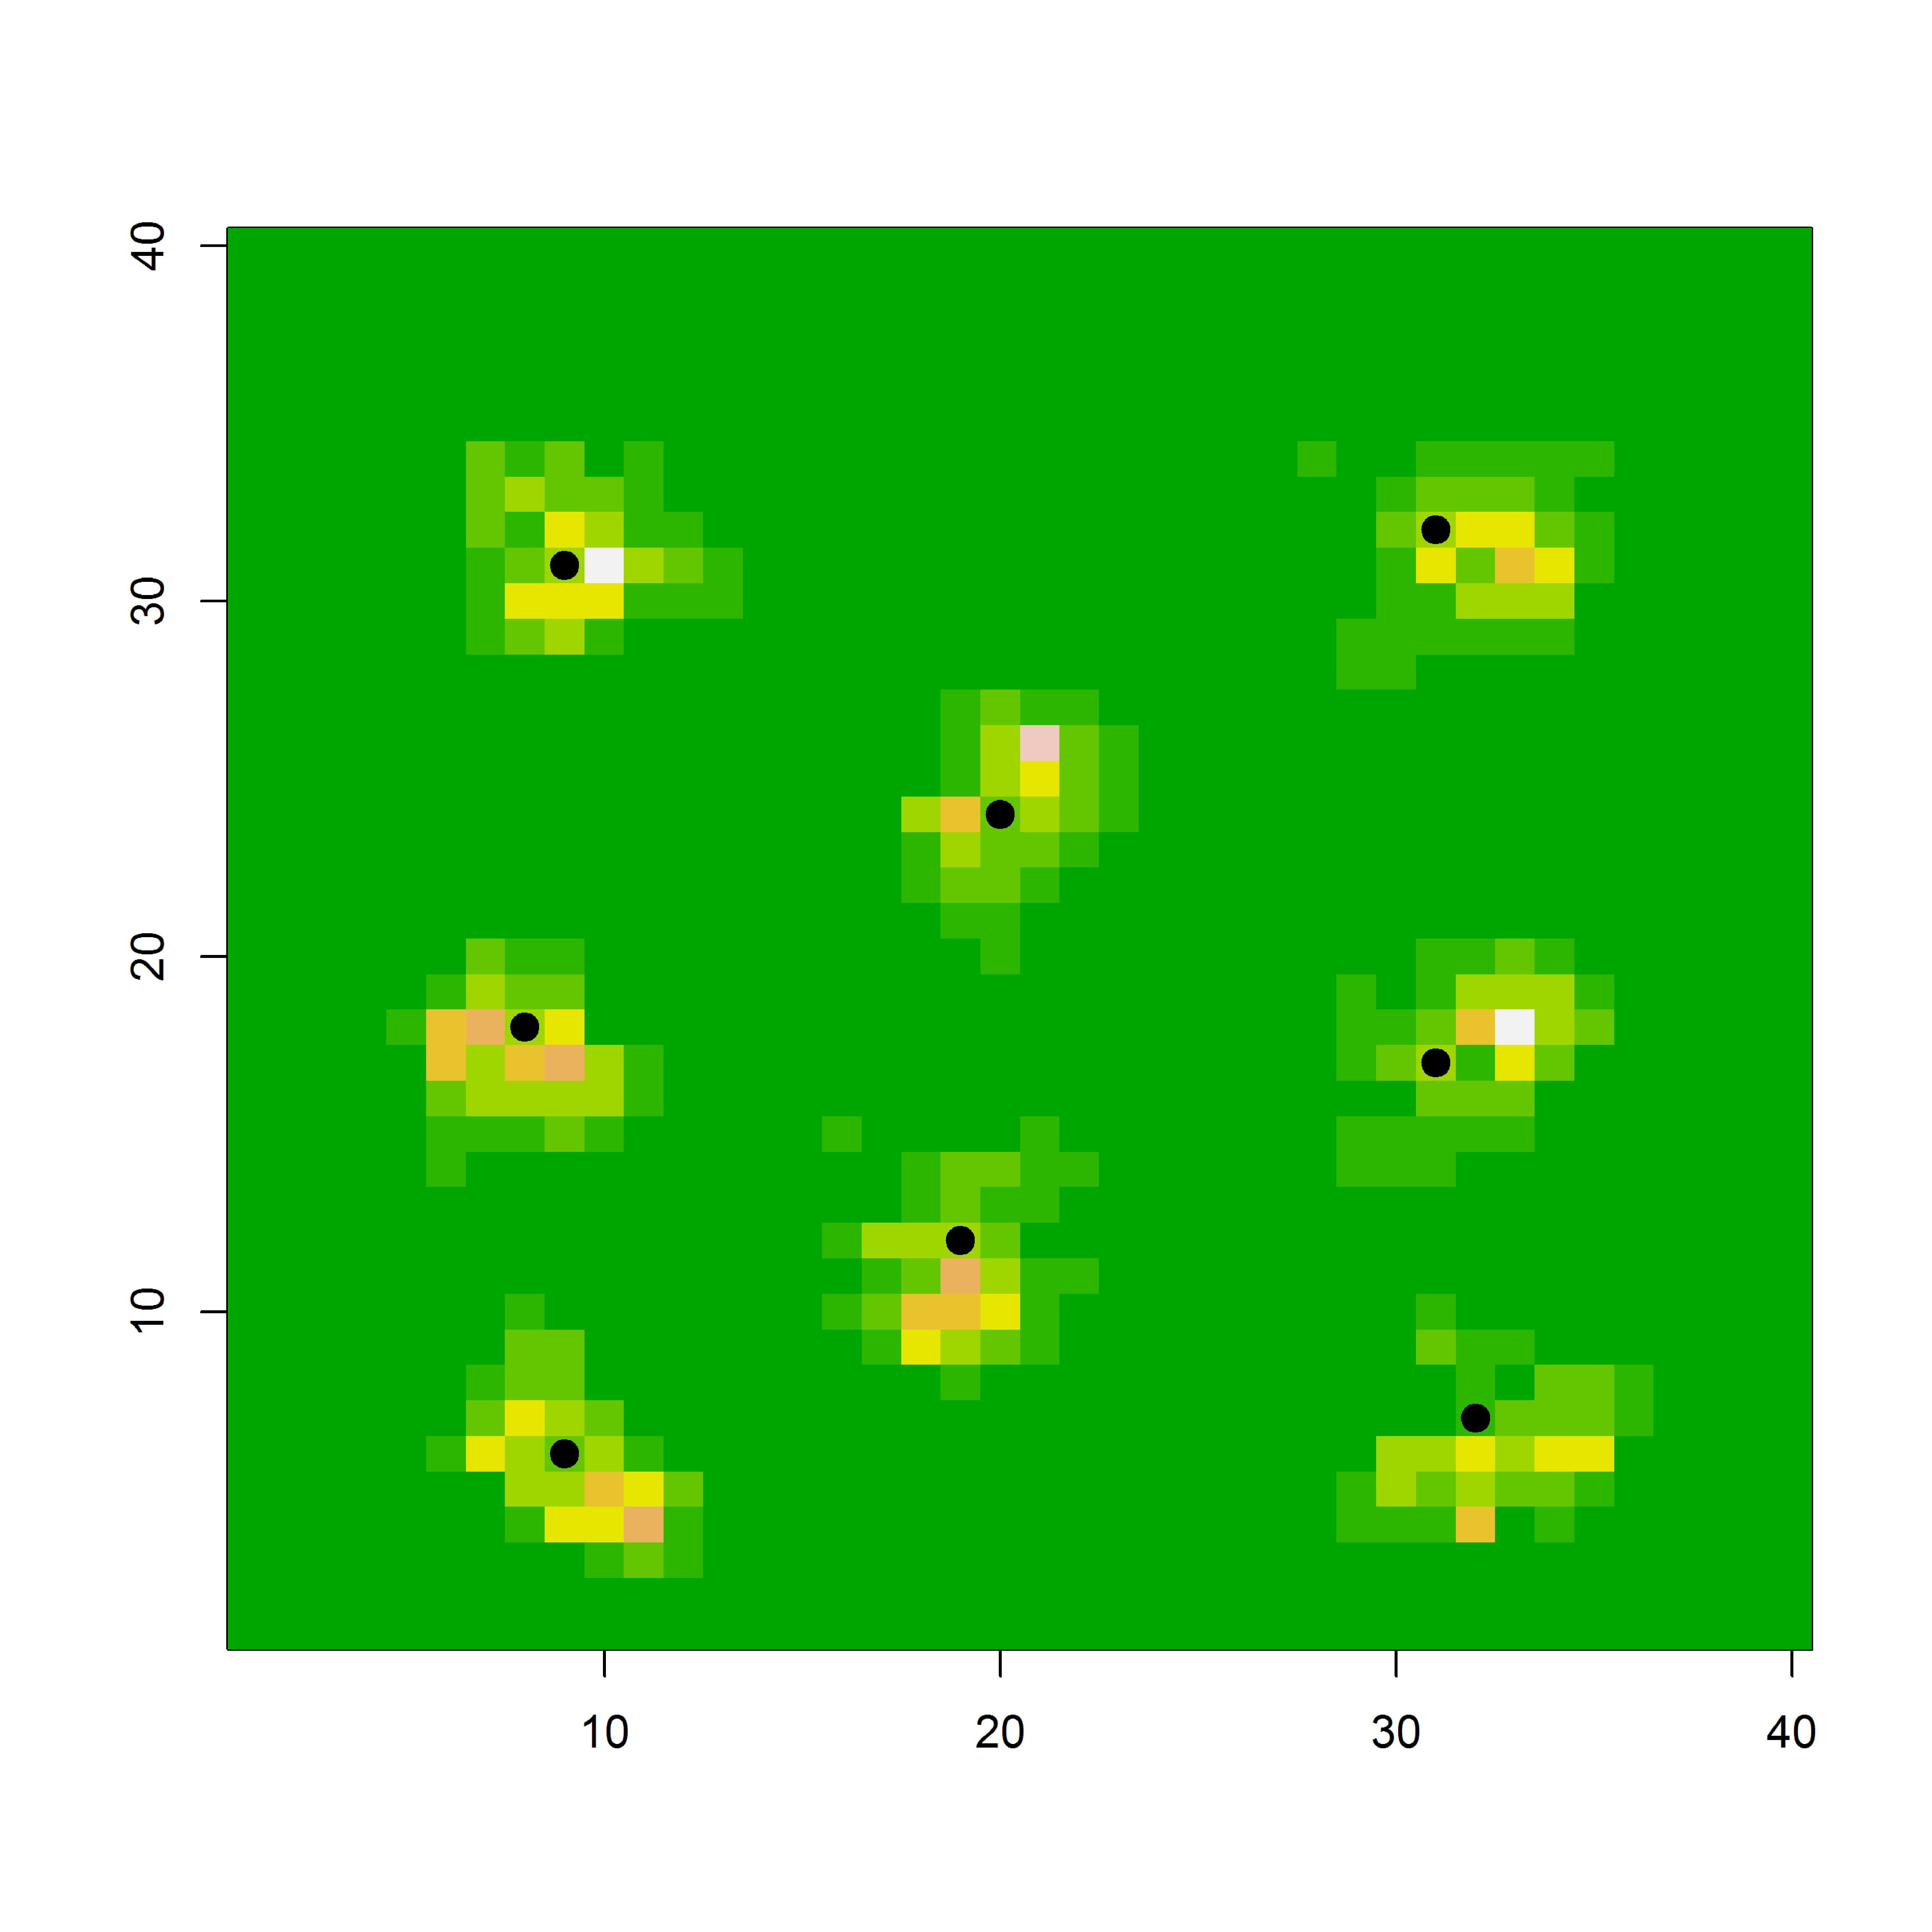
\includegraphics[width=3.5in,height=3.5in]{Ch13-RSF/figs/homeranges8}
\caption{Space usage patterns of 8 individuals under a space usage
  model that contains a single covariate which is shown in
  Fig. \ref{rsf.fig.habitat}. The plotted value is the multinomial
  probability $\pi_{ij}$ for pixel $j$ under the model in Eq. \ref{rsf.eq.rsf}.
}
\label{rsf.fig.homeranges}
\end{figure}
The covariate in this case was simulated using a kriging
model 
%XXX RS: What's a kringing model? what does that mean for the covariate? is it a gradient, random, spatially autocorrelated?  XXXX
with the following {\bf R} commands:
\begin{verbatim}
> set.seed(1234)
> gr <- expand.grid(1:40,1:40)
> Dmat<-as.matrix(dist(gr))
> V <- exp(-Dmat/5)
> z <- t(chol(V))%*%rnorm(1600)
\end{verbatim}
Home ranges shown in Fig.~\ref{rsf.fig.homeranges} were simulated
with $\alpha_{1} =
1/(2\sigma^2)$, with $\sigma = 2$, and the coefficient on $C({\bf x})$
set to $\alpha_{2} = 1$. The resulting space usage densities -- ``home ranges'' -- exhibit clear
non-stationarity in response to the structure of the underlying
covariate, and they are distinctly asymmetrical.  We note that if
$\alpha_{2}$ were set to 0, the 8 home ranges shown here would
be proportional to bivariate normal kernels with $\sigma = 2$.
The commands for the kringing model, and those to produce Fig. \ref{rsf.fig.habitat} are in
the package \mbox{\tt scrbook} (see \mbox{\tt ?RSF$\_$example}).
\begin{figure}[ht]
\centering
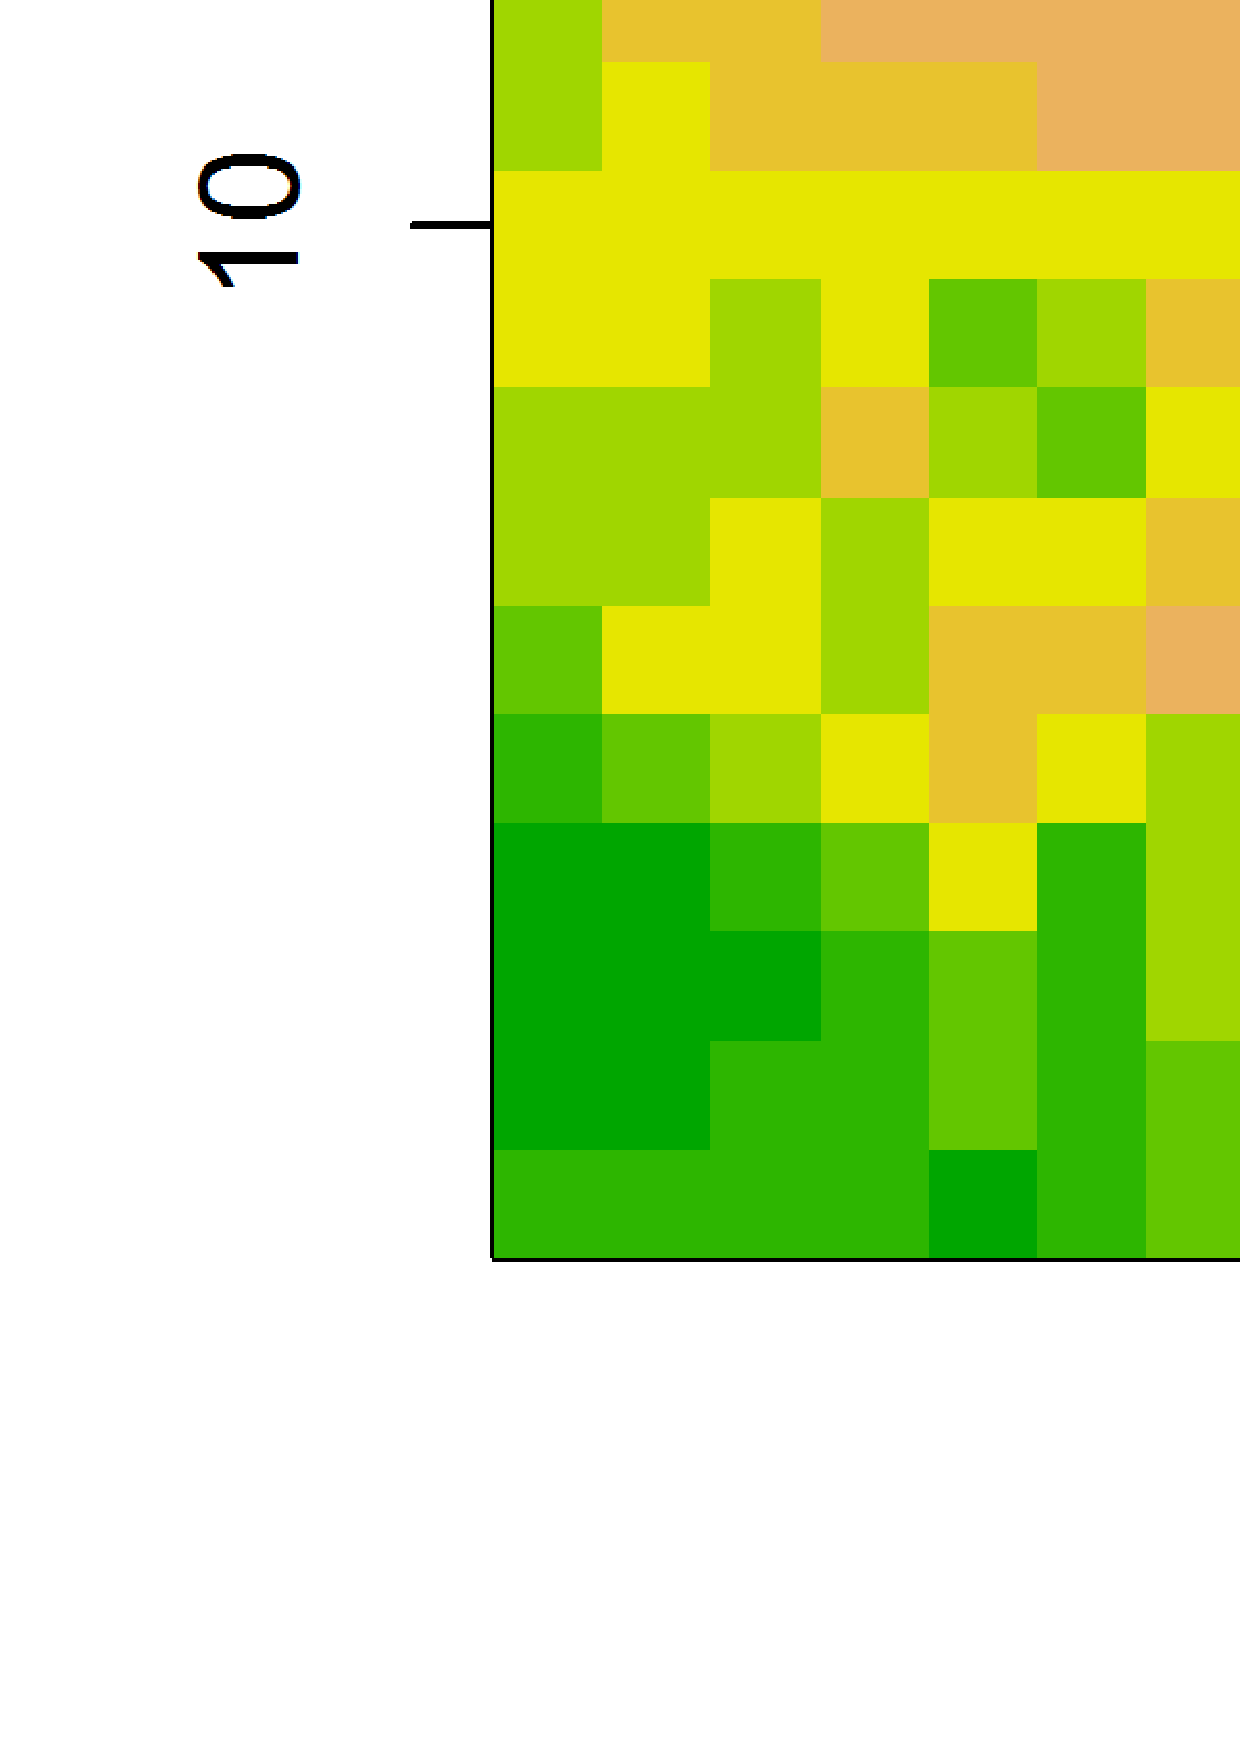
\includegraphics[width=3.15in,height=2.93in]{Ch13-RSF/figs/habitat.png}
\caption{A typical habitat covariate reflecting habitat quality or
  hypothetical utility of the landscape to a species under study. Home
  range centers for 8 individuals are shown with black dots.}
\label{rsf.fig.habitat}
\end{figure}
%XXX RS: I think I'd bring the habitat figure first, then the home ranges XXXX

\subsection{Poisson use model}
%XXRS: maybe Poisson model of space use XXX
A natural way to motivate the multinomial model of space usage is to
assume that individuals make a sequence of resource selection
decisions so that the outcomes $m_{ij}$ are {\it
  independent} Poisson random variables:
\[
 m_{ij} \sim \mbox{Poisson}( \lambda_{ij})
\]
where
\[
 \log(\lambda_{ij}) = a_{0} -\alpha_{1} d_{ij}^{2} +  \alpha_{2} C({\bf x}_{j})
\]
In this case, the number of visits to any particular cell is affected
by the covariate $C({\bf x})$ but has a baseline rate, $\exp(a_{0})$,
related to the amount (in an expected value sense) of movement occuring over some time interval.
This is an equivalent model to the multinomial model given previously
in the sense that, if we condition on the total sample size $R = 
\sum_{j} m_{ij}$, then the vector ${\bf m}_{i}$ has a multinomial
distribution with probabilities given by Eq. \ref{rsf.eq.rsf} (see
also Chapt. \ref{chapt.poisson-mn}).  Also note that if use
frequencies are summarized over individuals for each pixel, i.e.,
create the totals $m_{.j} = \sum_i m_{ij}$, then a standard Poisson
regression model for the resulting ``quadrat counts'' is
reasonable. This is ``Design I'' in \citet{manly_etal:2002}.
%XXX maybe say what design I relates to - is it RSF specific or something else?
%%% Richard: can you embellish this a little bit?
% XX RS: Agree: Needs one or two sentences on design 1; also, before you cite Johnson and his levels of selection, then Manly's protocoll A, now design 1. Would be nice to reconcile all those. Maybe a table with the definitions? It just gets messy with 3 different scales/structures for the same problem XXXX

In practice, we never observe ``truth'', i.e., the actual use
frequencies $m_{ij}$. Instead, we observe a sampling XXX sample? XXX of the actual use
outcomes by an individual.  As formulated in
Sec.~\ref{scr0.sec.implied}, we assume a binomial (``random'')
sampling model:
\[
 y_{ij} \sim \mbox{Binomial}(m_{ij}, p_{0}).
\]
We can think of these counts as arising by thinning the underlying
point process (here, aggregated into pixels) where $p_{0}$ is the
thinning rate of the point process.  
% XXX RS: So far we've used point process to describe distribution of s in S. But now you mean the telemetry locations, right? Would make that more explicit XXXXX
In this case, the marginal
distribution of the observed counts $y_{ij}$ is also Poisson but with mean
\[
 \log(\mathbb{E}(y_{ij}))  = \log(p_{0}) + a_{0} -\alpha_{1} d_{ij}^{2} +  \alpha_{2} C({\bf x}_{j}).
\]
Thus, the space-usage model (RSF) for the thinned counts $y_{ij}$ is
the same as the space-usage model for the original variables $m_{ij}$.
This is because if we remove $m_{ij}$ from the conditional model by
summing over its possible values, then the vector ${\bf y}_{i}$ is
{\it also} multinomial with cell probabilities
\[
\pi_{ij} = \frac{\lambda_{ij}}{\sum_{j} \lambda_{ij}}
\]
where any constant (the intercept term $a_0$ and thinning rate
$p_{0}$)
cancel 
from the numerator and denominator. Thus, the underlying multinomial
RSF model applies to the true unobserved count frequencies ${\bf
  m}_{i}$ and also those produced from thinning or sampling, ${\bf
  y}_{i}$.


\section{Integrating Capture-Recapture Data}

The key to combing RSF data with SCR data is 
to note that the Poisson model of space usage given above is 
exactly our Poisson encounter probability model from
Chapt. \ref{chapt.poisson-mn}, but with some arbitrary intercept off-set
related to the 
sampling rate by the telemetry device, and with
a spatial covariate  $C({\bf x})$.
We've used exactly this model for our SCR data (Chapt. \ref{chapt.covariates}), but with a different intercept,
$\alpha_{0}$, unrelated to the intercept of the Poisson use model
for telemetry described above but, rather, to the efficiency of the capture-recapture
encounter device. 
In other words, we view camera traps (or other devices) located in
some pixel ${\bf x}$ (or multiple pixels) as being equivalent to being able to turn on a
type of (less perfect) telemetry device only in that pixel.
%result of some thinning of the ``true'' space usage outcomes.
%In other words, imagine that we have a sampling device, such as a
%camera trap, in {\it every} pixel. If the device operates continually
%then it functions similar to a telemetry instrument in the sense that
%we can observe an individual in {\it any} pixel. But, given that 
%Given that real sampling devices
% operate imperfectly, intermittently, or do not expose the
%entire area of each pixel, then a reasonable model for this imperfect
%observation is the ``thinned'' binomial model given above, but with a
%different 
%intercept, say 
%representing the sampling
%effectiveness of the device, what we've called the baseline encounter
%rate in previous chapters. 
Therefore, 
data from a camera trapping are Poisson random variables 
for every pixel $j$ where a trap is located:
\[
y_{ij}|{\bf s}_{i} \sim \mbox{Poisson}( \lambda_{ij})
\]
with 
\[
 \log(\lambda_{ij}) =  \alpha_{0} -\alpha_{1}
 d_{ij}^{2} +  \alpha_{2} C({\bf x}_{j}).
\]
The parameters $\alpha_{1}$ and $\alpha_{2}$ are shared with the
multinomial model for the telemetry data.

Alternatively, 
the SCR study can produce binary 
encounters depending on the type of sampling being done,
where $y_{ij} = 1$ if the individual $i$ visited
the pixel containing a trap and was detected, then we imagine that
$y_{ij}$ is related to the latent variable $m_{ij}$ being the event
$m_{ij}>0$, which occurs with probability
\[
 p_{ij} = 1-\exp(- \lambda_{ij})
\]
%We combine the constants so that $\alpha_{0} = \log(\lambda_{0}) + a_{0}$
%is the baseline encounter rate which includes the constant intensity
%of use by the individual and also the baseline rate of detection,
%conditional on use.  The Bernoulli observation model implies that the
and then the observed encounter frequencies for individual $i$ and trap $j$, from
sampling over $K$ occassions are binomial:
\[
 y_{ij}|{\bf s}_{i} \sim \mbox{Binomial}(K, p_{ij}) 
\]

A key point here is that if resource selection is happening, then it
appears as a covariate on encounter rate (or encounter
probability) in the same way as ordinary covariates which were discussed in
Chapt. \ref{chapt.covariates}.


\subsection{The Joint RSF/SCR Likelihood}

To construct the likelihood for SCR data when we have 
direct information on space usage
from telemetry data, we regard the two samples (SCR and RSF) as
independent of one another, and we 
 form the likelihood for each set of observations as a function
of the same underlying parameters. The joint likelihood then is the
product of the two components. 

In particular, let ${\cal L}_{scr}(\alpha_{0}, \alpha_{1}, \alpha_{2}, N;{\bf y})$
be the likelihood for the SCR data in terms of the basic encounter
probability parameters and the total (unknown) population size $N$,
and let ${\cal L}_{rsf}(\alpha_{1},\alpha_{2}; {\bf m})$ be the
likelihood for the RSF data based on telemetry which, because the
sample size of telemetered individuals is fixed, does not depend on $N$.
Assuming independence of the two datasets, the
joint likelihood is the product of these two pieces:
\[
{\cal L}_{rsf+scr}(\alpha_{0},\alpha_{1},\alpha_{2},N; {\bf y},{\bf
  m})  =
{\cal L}_{scr}(\alpha_{0}, \alpha_{1}, \alpha_{2}, N;{\bf y})
\times
{\cal L}_{rsf}(\alpha_{1},\alpha_{2}; {\bf m}),
\]
where the ${\cal L}_{scr}$ is the standard integrated likelihood
(Chapt. \ref{chapt.mle}), and the RSF likelihood contribution is the
multinomial telemetry likelihood having cell probabilities
Eq. \ref{rsf.eq.rsf}.  The {\bf R} code for this 
%XXX to maximize the joint likelihood? or for what? XXX 
was given in the
supplement to \citet{royle_etal:2012mee}, and we include a version of
this in the \mbox{\tt scrbook} package, see \mbox{\tt ?intlik3rsf},
which also shows how to simulate data and fit the combined SCR+RSF
model.

%XXX a lot of our book is from papers, but this section below sounds
%particularly like we didn't try.  I revised it a bit, hope you think it's okay

\section{SW  New York Black Bear Study}
\label{rsf.chapt.nybears}

\citet{royle_etal:2012mee} applied the integrated SCR+RSF model to
data from a study of black bears in a region of approximately 4,600
km$^2$ in southwestern New York \citep{sun:2013}\footnote{This is
different from our Fort Drum bear study data set which we've analyzed
in previous chapters}.  The data can be loaded from the \mbox{\tt scrbook}
library with the command \mbox{\tt data(nybears)}.
We reproduce the findings of \citet{royle_etal:2012mee} in this section.

The data are based on a noninvasive genetic capture-recapture study
using 103 hair snares in June and July, 2011.  Hair snares were baited
and scented and checked weekly for hair \citep{sun:2013}.  The study
yielded relatively sparse encounter histories
 of 33 individuals with a total of 14 recaptures (27
individuals captured 1 time only.
% Extra trap recaptures included  %XXX what is an extra trap recap?
%3 individuals captured in 2 traps, 1 individual in each of 3 and 4
%traps).  
Telemetry data were collected on 3 telemetry-collared individuals, which produced
locations for each bear approximately once per hour.  We 
thinned these data to once per 10 hours to produce movement outcomes that might
be more independent. This produced 195 telemetry locations used in the
RSF component of the model.  Elevation was used as the covariate for this 
model, a standardized version of which is shown in
Fig. \ref{fig.elevation} along with the locations of each
capture at hair snare sites.  


\begin{figure}[ht]
\centering
\includegraphics[width=3.25in,height=3.25in]{Ch13-RSF/figs/elev_captures_bw.png}
\caption{
Elevation (standardized), hair snare locations (indicated by ``$x$'') and location
of bear captures (open circles).
Multiple captures at a trap location are offset by adding
random noise.
}
\label{fig.elevation}
\end{figure}

%XXXX RS: I think this figure needs some work; symbols are difficult to distinguish. XXXX

There are a number of models that could be fitted to these data based on
the combination of SCR and RSF data as well as the elevation covariate.  
The models fit here are
 based on the Gaussian hazard trap encounter/space usage model,
including an ordinary SCR model with no covariates or telemetry data,
the SCR model with elevation affecting either $\lambda_{0}$ or density
$D({\bf x})$ (Chapt. \ref{chapt.state-space}), and models that use
telemetry data.  The 6 models fitted were:
\begin{itemize}
\item[] Model 1,  SCR: ordinary SCR model
\item[] Model 2, SCR+p(C): ordinary SCR model with elevation as a
  covariate on baseline encounter probability $\lambda_{0}$.
\item[] Model 3, SCR+D(C): ordinary SCR model with elevation as a
  covariate on density only.
\item[] Model 4, SCR+p(C)+D(C): ordinary SCR model with elevation as
  a covariate on both baseline encounter probability and density.
\item[] Model 5, SCR+p(C)+RSF: SCR model including data from 3
  telemetered individuals.
\item[] Model 6, SCR+p(C)+RSF+D(C): SCR model including telemetered
  individuals and with elevation as a covariate on density.
\end{itemize}
It is tempting to want to compare these different models by AIC but,
because models 5 and 6 involve additional data, they cannot be
compared with models 1-4.  Parameter estimates for the six models are
given in Table \ref{tab.nyresults} (reproduced from
\citet{royle_etal:2012mee}, see also the help file \mbox{\tt
  ?nybears}).

By looking at Table \ref{tab.nyresults}, it is clear based on the
negative log likelihood for just Models 1-4, that those containing an
elevation effect on density are preferred (Model 3 and 4).  The
parameter estimates indicate a positive effect of elevation on
density, which seems to be consistent with the raw capture data shown
in Fig. \ref{fig.elevation}.  Despite this strong effect
of elevation, the estimates of $N$ under each of these models only
ranged from $93 - 103$ bears for the 4600 km$^2$ state-space.
%XXX RS: So density is pretty constant across models? XXX
  If we
consider not just density, but space usage (i.e., looking at the
parameter $\alpha_2$), the effect of elevation is negative.  Thus, elevation, appears to affect density and space usage
differently.  It was suggested that density operates at the
second-order scale of resource selection and ``....is largely related
to the spacing of individuals and their associated home ranges across
the landscape.  On the other hand, our RSF was defined based on
selection of resources within the home range (third-order).''
\citep{royle_etal:2012mee} 
%XXXX RS: Since you bring up second-order resource selection here, the different orders def. need to be defined earlier on XXX
The positive effect of density on elevation
is consistent with some other studies XXX on black bears? XXXX \citep[e.g.][]{frary_etal:2011},
and the negative effect of elevation on space usage can be attributed to
seasonal variation in food availability, usage of corridors, or
environmental conditions.


Models 5 and 6 include the additional telemetry data, thus the
negative log-likelihoods are not directly comparable to the first 4
models, but we can still make a few important observations.  First is
that the parameter estimates under these two models are consistent
with Model 4 in that elevation had a strong effect on both density and
space usage.  In comparing models 5 and 6, the latter model which
includes elevation as an effect on density reduces the negative
log-likelihood by 5 units.  Additionally, including the telemetry data
reduces the standard errors (SE) of the density and space usage
parameters and as we would expect, the incorporation of telemetry data
also reduces the SE for $\sigma$.  The increased precision for the
estimated population size ($N$) is negligible with the use of
telemetry data in this case.  However, that may be different if more
telemetry information were available.  Model 6 (SCR+p(C)+RSF+D(C)),
was used to produce maps of density (Fig. \ref{fig.density}) and space
usage (Fig. \ref{fig.spaceusage}) showing the effect of elevation on
both components of the model.  The map of space usage shows the
relative probability of using a pixel ${\bf x}$ relative to one having
the mean elevation, given a constant distance to the individual's
activity center.
 %XXXX is that a correct interpretation of what you did?


\begin{comment}

XXX Beth: I rewrote all of this above  
XXX you can put it all back in and take my stuff out if you want

{\bf XXXXXXXX below is exactly plagarized from the paper XXXXXXXXXXXX}
Looking at  models 1-4, which do not use the telemetry observations,
models in which elevation effects density are preferred, and we see a
a large positive response to elevation, which is apparent in
consistent with the visual pattern apparent in
Fig. \ref{fig.elevation} (more captures at higher elevations).
Conversely,
there is a negative effect of elevation on
space usage (the parameter $\alpha_{2}$).
The estimate of $N$ for the 4600 km$^2$ state-space, based on the best
model is about 103 bears $(\exp(4.25)+33)$.
In the two models that include the additional telemetry data, a couple
points stand out: Clearly the elevation effect on density is
important, reducing the negative log-likelihood by 5 units. The effect
of elevation on density and space usage are roughly consistent with
Model 4 which did not use telemetry data. Furthermore, the standard
errors (SE) of those two parameter estimates are reduced considerably
when the model uses telemetry data, as is the SE for estimating
$\log(\sigma)$.  The SE for estimating $\log(n_{0})$ is only improved
incrementally compared to the models without telemetry data.  We used
the best model, \mbox{\tt SCR+p(C)+RSF+D(C)}, to produce a map of
density (Fig. \ref{fig.density}) which shows clearly the pattern
induced by elevation. We also produced a map
(Fig. \ref{fig.spaceusage}) to illustrate the effect of elevation on
space usage. This shows the relative probability of using a pixel
${\bf x}$ relative to one of mean elevation, and of the same distance
from an individual's activity center.
% remind people how to compute "the relative prob of using pixel x XXXX
%The cool thing about these models is we can make pretty
%multi-colored maps of things.  A map of density under the
%model is shown in fig. \ref{fig.density}.  A map of space usage in
%terms of the relative probability of using pixel $x$ relative to the
%average pixel is shown in Fig. \ref{fig.spaceusage}.

\end{comment}

\begin{comment}
I computed the MLE of N and the SE using a delta approximation as
follows: The MEE paper has log(n0) and the se of log(n0) which is not informative.
> logn0<-c(4.140,4.110,4.114,4.255,3.884,4.028)
> sev<- c(0.366,0.362,0.358,0.377,0.363, 0.366)
> exp(logn0)+33
[1]  95.80282  93.94672  94.19099 103.45682  81.61830  89.14850
> sev*exp(logn0)
[1] 22.98583 22.06271 21.90638 26.56222 17.64844 20.55035
\end{comment}

%XXX RS: Table seems to wide and seems to have a different format from rest of the book (vertical line, more horizontal lines ) XXX
\begin{table}
\centering
\caption{
Summary of model-fitting results for the black bear study. Parameter
estimates are for the intercept ($\alpha_{0}$), logarithm of $\sigma$,
the
scale parameter of the Gaussian hazard encounter model, 
 $\beta$ is the coefficient of elevation on density, and the total
 population size $N$ of the state-space. Standard errors
 rae in parentheses.
The SCR data are based on $n=33$ individuals, and the telemetry data
are based on 3 individuals. 
}
\begin{tabular}{c|rrrrrr}
\hline \hline
model         & $\alpha_0$ & $\log(\sigma)$ & $\alpha_{2}$ & $N$ & 
$\beta$       & -loglik                                                                         \\ \hline
SCR(elev)      & -2.860    & -1.117        & 0.175       & 95.8        &        & 122.738  \\
             &  (0.390)     & (0.139)       & (0.248)       & (22.99)        &        &           \\
SCR          & -2.729    & -1.122        & ---          & 93.9        &        & 122.990  \\
              & (0.345)     & (0.140)       &              & (22.06)        &        &           \\
SCR+D(elev)      & -2.715    & -1.133        & ---          & 94.2        & 1.247 & 118.007  \\
              & (0.353)     & (0.139)       &              & (21.90)    & (0.408) &           \\
SCR(elev)+D(elev) & -2.484    & -1.157        & -0.384      & 103.5        & 1.571 & 117.075  \\
              & (0.391)     & (0.142)       & (0.276)       & (26.56)   & (0.463) &           \\
SCR(elev)+RSF       & -3.068    & -0.814        & -0.281      & 81.6        &        & 1271.739 \\
              & (0.272)    & (0.036)         & (0.118)       & (17.65)        &        &           \\
SCR(elev)+RSF+D(elev)  & -3.070    & -0.810        & -0.371      & 89.1        & 1.273 & 1266.700 \\
              & (0.272)    & (0.037)         & (0.124)       & (20.55)        & (0.411) &           \\
\hline
\end{tabular}
\label{tab.nyresults}
\end{table}



\begin{figure}
\centering
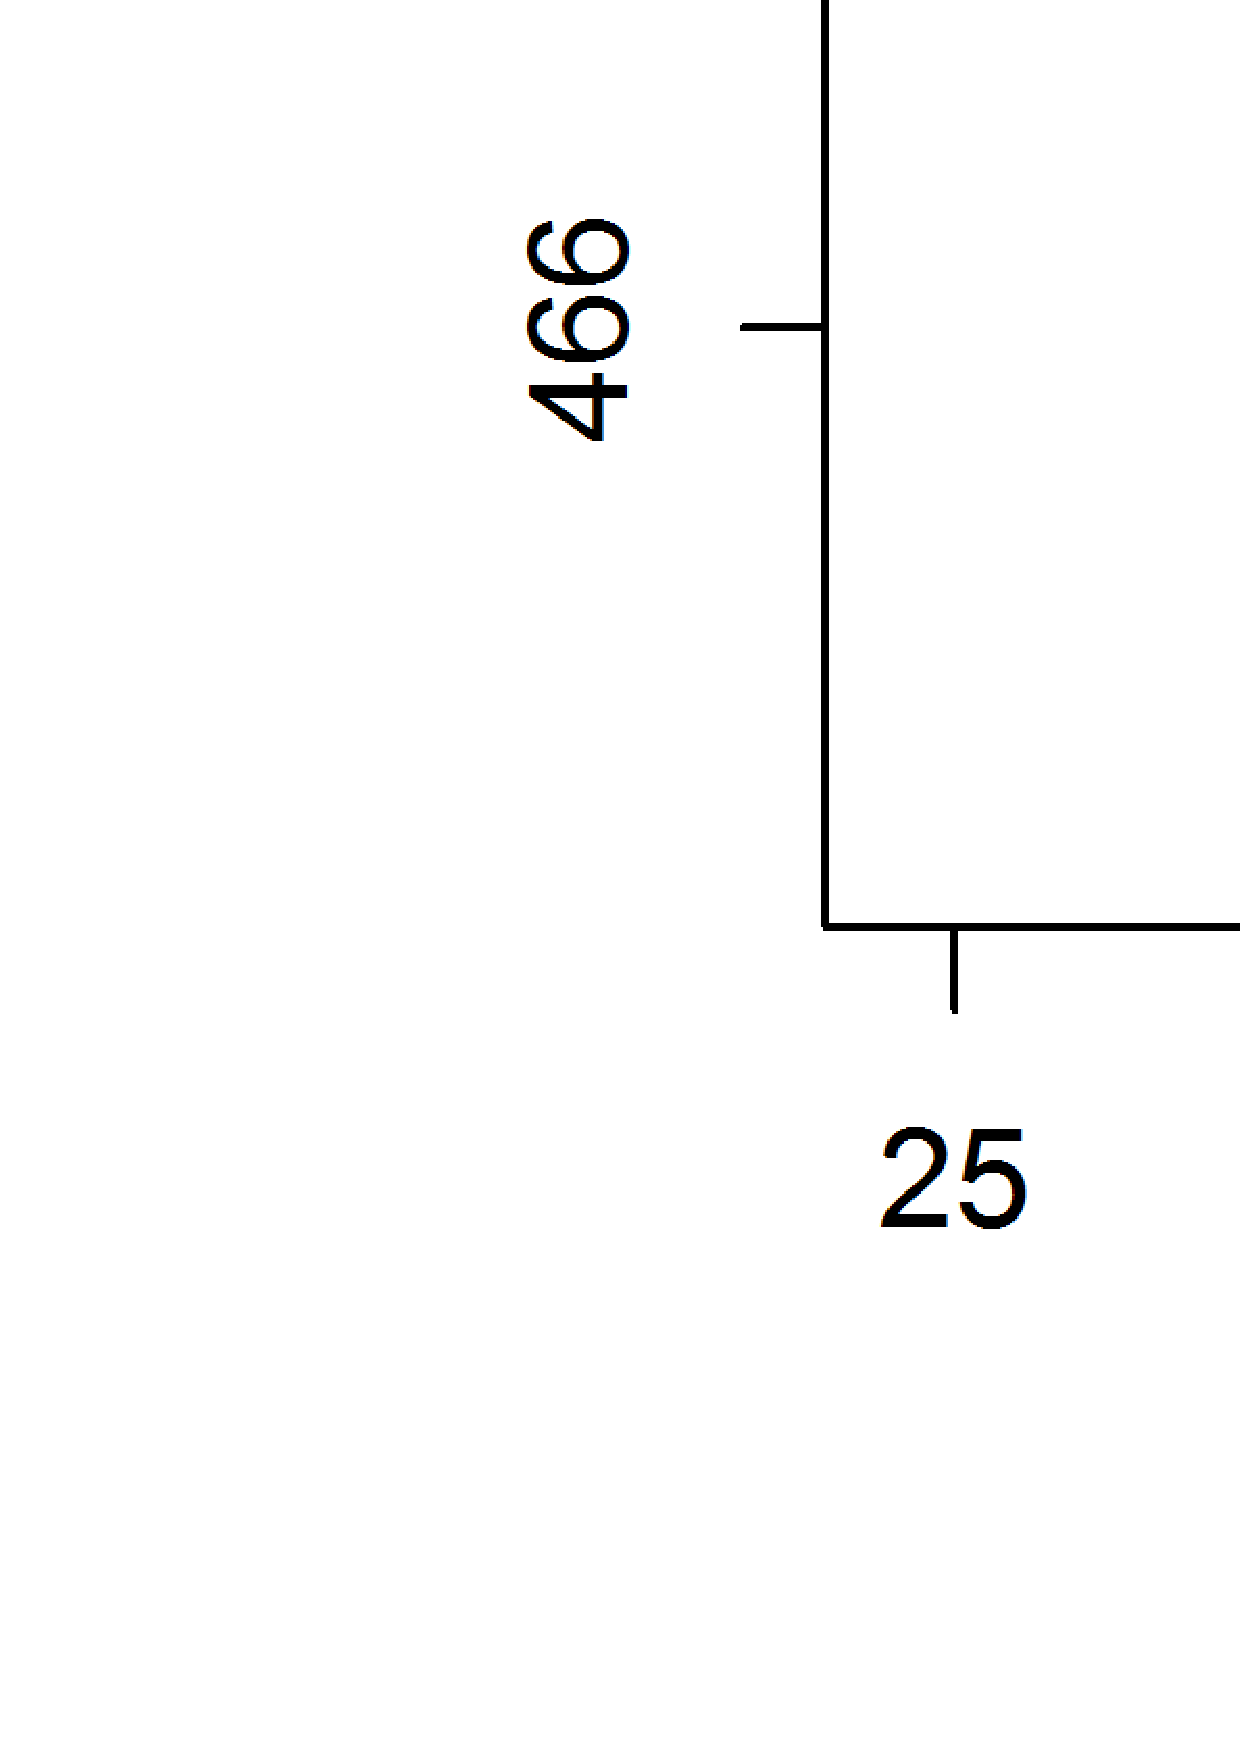
\includegraphics[width=3.25in,height=3.25in]{Ch13-RSF/figs/density2.png}
\caption{Predicted density of black bears (per 100 km$^2$) in
  southwestern  New York study
  area.
}
\label{fig.density}
\end{figure}


\begin{figure}
\centering
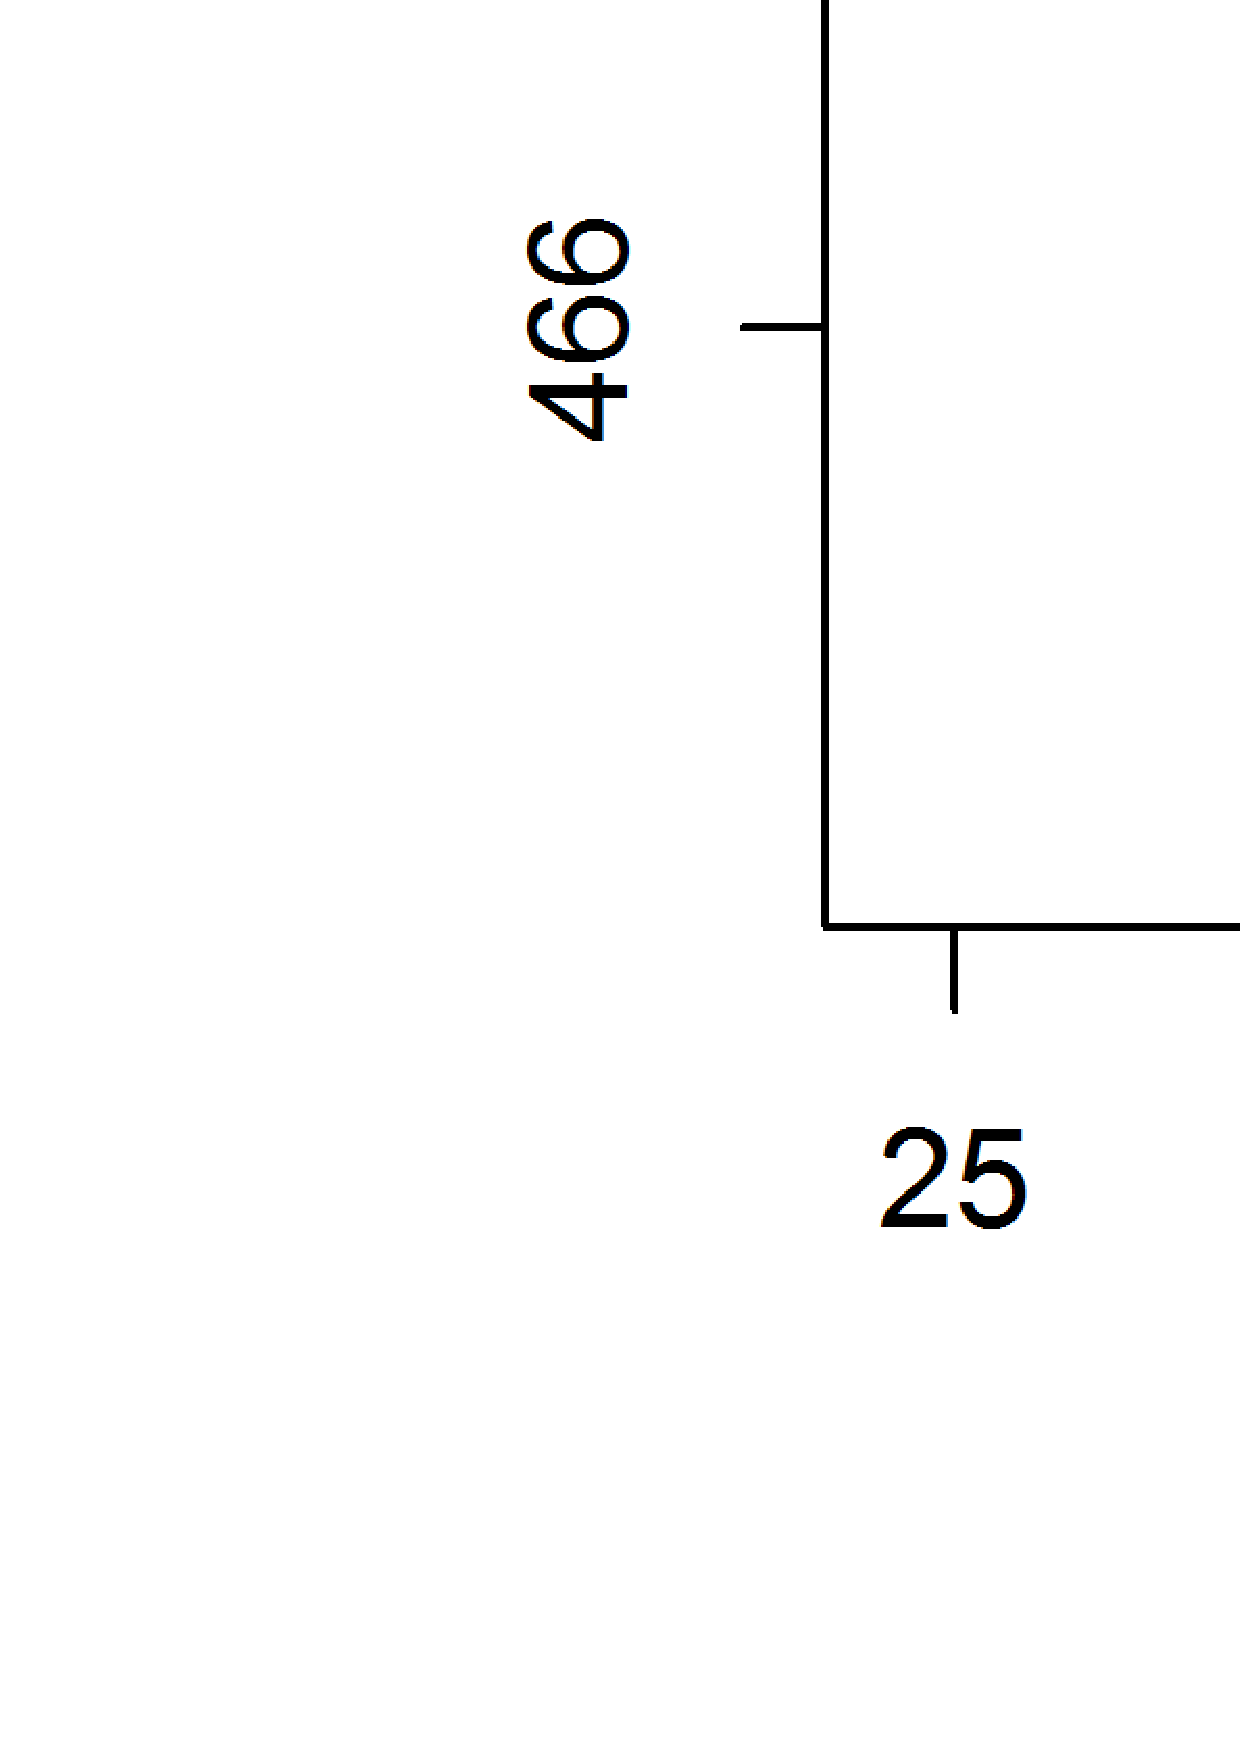
\includegraphics[width=3.25in,height=3.25in]{Ch13-RSF/figs/spaceusage2.png}
\caption{Relative probability of use of pixel ${\bf x}$ compared to a pixel
  of mean elevation, at a constant distance from the activity center.
}
\label{fig.spaceusage}
\end{figure}



\section{Simulation Study}

Using the simulated landscape shown in Fig. \ref{rsf.fig.habitat},
\citep{royle_etal:2012mee} presented results of a simulation study
considering populations of $N=100$ and $N=200$ individuals
%To
%simulate encounter data, a $7 \times 7$ array of trapping devices was
%located on the the integer coordinates $(u*5,v*5)$ for $u,v =
%1,2,3,4,5,6,7$ and sampling was conducted for $K=10$ periods.  For the
%XX RS: I would put the details back in; maybe not the integer coordinates, but the array and K for sure XXX
using the Gaussian hazard mode:
\[
\mbox{cloglog}(p_{ij}) = -2  -\frac{1}{2\sigma^{2}} d_{ij}^{2} + 1 \times C({\bf x}_{j}).
\]
with $\sigma =2$.
Recall, that $\mbox{cloglog}(u) =
\log(-\log(1-u))$ is the complementary log-log function.
%XXX I reworded the above to make it clearer (it was kind of a long sentence before)
% Also, the cloglog is not previously used in this chapter so we might want
% to directly relate it to your equation in \section{Integrating Capture-Recapture Data}
In the absence of selection (omitting the covariate $C({\bf x})$),
this model corresponds to a space usage model that is bivariate normal
with standard deviation 2 (Sec. \ref{scr0.sec.implied}).

Using this model, \citet{royle_etal:2012mee} looked at the effect of
misspecification of the resource selection model with an ordinary
model SCR0 (i.e. no habitat covariates affecting the trap encounter model), and the peformance of the MLEs, under SCR+telemetry
designs having 2, 4, 8, 12, and 16 telemetered individuals (with 20
independent telemetry fixes {\it per} individual). 
\citet{royle_etal:2012mee} fitted 3 models: (i) the SCR only model, in which the telemetry
data were not used; (ii) the integrated SCR/RSF model which combined
all of the data for jointly estimating model parameters; and (iii) the
RSF only model which just used the telemetry data alone (and therefore the parameters
$\alpha_{0}$ and $N$ are not estimable).  An abbreviated
version of the results from \citet{royle_etal:2012mee} is summarized
in Table \ref{rsf.tab.sims} below. We provide an {\bf R} script (see \mbox{\tt
  ?RSFsim}) that can be modified for further analysis and exploration.

One thing we see is a pretty dramatic XXX negative? positive? XXX bias in estimating $N$ if the
 model SCR0 is fitted (interestingly, there is much less bias in
estimating $\sigma$).  Overall, though, when either the SCR model with
covariate or the joint SCR+RSF model is fitted, the MLEs exhibit
little bias for the parameter values simulated here. In terms of RMSE,
there is only a slight $\approx$ 5\% reduction in RMSE of the
estimator of $N$ when we have at least 2 telemetered individuals, and
as much as a 10\% reduction as in the $N=200$ situations.
%XXX RS: Not really clear - so up to 5 percent with N=100, and up to 10 percent for N=200? XXXX
 This makes
sense because we nail down the parameters and still don't know where
guys are, and get info about mean $p$, i.e. $\alpha_{0}$, only from the
SCR data. 
%XXX RS: the previous sentence needs some rewording; it's unclear which parameters we nail and under what scenario XXX
Thus estimating $N$ benefits only slightly from the addition
of telemetry data.  However, there is a large improvement (50-60\%) XXX in precision? XXX in
estimating the home range parameter $\sigma$.  While this doesn't
translate much into improved estimation of $N$, it suggests that it
should be relevant to the design of SCR studies for which trap spacing
is one of the main considerations (Chapt. \ref{chapt.design}). In terms of study design these results also
suggest that, perhaps, spatial recaptures are not needed if some
telemetry data are available (in Chapt. \ref{chapt.partialID}, in the context of mark-resight models, we show a case study of raccoons where additional telemetry data allows estimating model parameters in spite of a very low number of spatial recaptures \citep{sollmann_etal:2012ecol}). The resource selection parameter
$\alpha_{2}$ is well-estimated even {\it without} telemetry data. The
fact that parameters of resrouce selection can be estimated from
ordinary capture-recapture data should have considerable practical
relevance in the study of animal populations and landscape
ecology. For the highest sample size of telemetered individuals
($n=16$), the RMSE for estimating this parameter only decreases from
about $0.09$ to $0.07$.



\begin{table}[ht]
\centering
\caption{
  This table summaries the sampling distribution of the MLE of model
  parameters   for models fitted to data generated under a resource selection model.
  The models fitted   include the misspecified model, which is a basic model SCR0 (with no covariate), the SCR model with
  the covariate on encounter probability, and the SCR model including
  the covariate and a sample of telemetered individuals ($n$ is the
  number of individuals telemtered).    Data were simulated with   $N=200$ individuals,
  $\alpha_{2} = 1$ and $\sigma = 2$.
}
\begin{tabular}{ccccccc} \hline \hline 
        &  $\hat{N}$ &RMSE   &  $\hat{\alpha}_{2}$ &RMSE  &        $\hat{\sigma}$ & RMSE    \\ \hline
n=2     &       &       &       &      &        &         \\
SCR+C(x)& 199.11&  14.28&  0.99 &  0.09&   2.00 &  0.090  \\
SCR+RSF & 199.11&  13.80&  0.99 &  0.09&   2.00 &  0.079  \\
SCR0    & 161.48&  39.98&   --  &   -- &   1.84 &  0.180  \\ \hline
n=4   &       &      &        &    &        &          \\
SCR only& 199.67&  13.87&   1.00&   0.09 &  2.00&   0.090 \\
SCR/RSF & 199.65&  13.59&   1.00&   0.09 &  2.00&   0.072\\
SCR0    & 161.32&  40.00&    -- &    --  &  1.83&   0.191\\ \hline
n=8    &       &      &        &    &        &          \\
SCR only& 199.24&  15.49&   0.99&   0.10&   2.01&   0.093 \\
SCR/RSF & 199.55&  14.17&   0.99&   0.08&   2.00&   0.063\\
SCR0    & 161.46&  40.06&    -- &    -- &   1.84&   0.184\\ \hline
n=12    &       &      &        &    &        &          \\
SCR only& 200.41&  15.16&   0.99&   0.10&   2.00&   0.086\\
SCR/RSF & 200.95&  13.04&   1.00&   0.08&   2.00&   0.051\\
SCR0    & 162.40&  38.95&    -- &    -- &   1.84&   0.185\\ \hline
n=16     &       &      &        &    &        &          \\
SCR only &199.16 & 15.62&   1.00 &  0.09&   2.00&   0.095 \\
SCR/RSF  &199.63 & 13.38&   1.00 &  0.07&   2.00&   0.052\\
SCR0     &160.93 & 40.44&    --  &   -- &   1.84&   0.190\\ \hline
\end{tabular}
\label{rsf.tab.sims}
\end{table}





























\begin{comment}
N=100, 300 iters each, mean SCR only N: 99.418     N=200, 500 iters. Mean SCR only N = 199.712
n=2          Nhat RMSE  ahat RMSE  sighat  RMSE    Nhat RMSE  ahat RMSE  sighat  RMSE
SCR only:   99.73  9.97  0.99  0.14  2.00  0.124  198.85  14.24   0.99   0.10   2.00   0.091
SCR/RSF:    99.94  9.54  0.99  0.12  2.00  0.097  199.37  12.80   0.99   0.09   2.00   0.078
sbar        98.89  9.50  0.93  0.14  1.97  0.100  197.87  13.94   0.96   0.10   1.99   0.080
RSF only     --    --    1.03  0.33  2.00  0.160    --      --    1.04   0.33   1.99   0.169
n=4
SCR only    99.10  9.83  0.99  0.13  2.00  0.127  200.06  15.34   1.00   0.09   2.00   0.092
SCR/RSF     99.17  9.47  0.99  0.11  2.00  0.086  200.25  14.36   1.00   0.08   2.01   0.073
sbar        97.43  9.68  0.89  0.16  1.97  0.090  198.14  14.31   0.94   0.10   1.98   0.075
RSF only     --     --   0.98  0.22  2.00  0.119    --     --     1.02   0.21   2.01   0.122
n=8
SCR only    99.59 10.00  1.00  0.13  2.00  0.130  200.85  14.06   1.00   0.09   2.00   0.087
SCR/RSF     98.90 10.02  0.99  0.10  2.00  0.071  200.29  13.98   1.00   0.08   2.00   0.061
sbar        96.07 10.37  0.84  0.19  1.96  0.078  196.46  14.59   0.90   0.13   1.97   0.069
RSF only     --    --    0.98  0.16  2.01  0.084    --     --     0.99   0.16   2.00   0.084
n=12
SCR only    99.44 10.73  0.98  0.13  2.02  0.128  198.76  14.47   0.99   0.10   2.00   0.091
SCR/RSF     99.96 10.26  1.00  0.09  2.00  0.059  198.72  14.14   1.00   0.08   2.00   0.054
sbar        96.30 10.49  0.82  0.20  1.96  0.071  193.83  15.14   0.87   0.15   1.97   0.063
RSF only     --    --    1.01  0.12  2.00  0.069    --     --     1.01   0.13   2.00   0.069
n=16
SCR only    99.23 10.74  0.99  0.14  2.00  0.128  200.04  14.09   0.99   0.10   2.01   0.088
SCR/RSF     99.20  9.79  1.00  0.09  1.99  0.057  200.25  13.40   1.00   0.07   2.00   0.047
sbar        95.10 10.17  0.80  0.22  1.95  0.075  194.38  14.26   0.85   0.17   1.96   0.059
RSF only     --    --    1.00  0.10  1.99  0.061    --     --     1.00   0.11   2.00   0.055





Results for $N=100$, $N=200$ and $N_{tel}=(2,4,8,12,16)$ are presented
in Table \ref{tab.results1}. We note that the first row of each batch
(labeled ``\mbox{\tt SCR only}'') represent the same estimator and data
configuration. These replicate runs of the SCR-only situation give us
an idea of the inherent Monte Carlo (MC) error in these simulations, which is
roughly about 0.25 and 0.89 on the $N$ scale for the $N=100$ and
$N=200$ cases, respectively.  The mean $N$ for the SCR-only
estimator across all 5 simulations for $N=100$ was
$\mbox{mean}(\hat{N}) = 99.418$, an empirical bias of $0.6\%$. For
$N=200$, the estimated $N$ across all 5 simulations (5 levels of
$N_{tel}$) was $\mbox{mean}(\hat{N}) = 199.712$, an empirical bias of
about $0.15\%$, within the Monte Carlo error of the true value of $N=200$.  The
results suggests a very small bias of $< 1\%$ in the MLE of $N$ for
both the  SCR-only and combined SCR/RSF estimators.  In practice, we
expect a small amount of bias in MLEs as likelihood theory only
guarantees asymptotic unbiasedness.


In terms of RMSE for estimating $N$, we see that (Table
\ref{tab.results1}), generally, there is about a 5\% reduction in RMSE
when we have at least 2 telemetered individuals. And, although there
is a lot of MC error in the RMSE quantities, it might be as much as a
10\% reduction as the sample size of captured individuals increases
under the higher $N=200$ setting. This incremental improvement in RMSE
of $\hat{N}$
makes sense because, while the
telemetry provides considerable information about the structural
parameters of the model, it provides no information about mean $p$,
i.e. $\alpha_{0}$, which comes only from the SCR data. Thus estimating
$N$ benefits only slightly from the addition of telemetry data.


The MLE of the RSF parameter $\alpha_{2}$ exhibits negligible or no
bias under {\it both} the SCR only and SCR/RSF estimators. It is
well-estimated from SCR data alone and even better than RSF data alone
(in terms of RMSE) until we have more than 200 or so telemetry
observations\footnote{This may appear pardoxical, but the SCR study is
  generating more spatial locations of individuals than the telemetry
  study based on 2 or 4 individuals}.  The biggest improvement from the use of telemetry data
comes in estimating the parameter $\sigma$. We see that $\hat{\sigma}$
is effectively unbiased, and there is a very large improvement in RMSE
of $\hat{\sigma}$, perhaps as much as 50-60\% in some cases, when the
telemetry data are used in the combined estimator (that does not
translate much into improvements in estimating $N$ as we saw
previously).  Improvement due to adding telemetry data diminishes as
the expected sample sizes increases, and so telemetry data does less
to improve the precision of $\hat{\sigma}$ and $\hat{\alpha}_{2}$ for
$N=200$ than for $N=100$. This is because the SCR data alone are
informative about both of those parameters.


The results as they concern likelihood estimation of $N$ suggest that
there is not a substantial benefit to having telemetry
data. Estimators ``SCR only'' and ``SCR/RSF'' both appear
approximately unbiased for $N=100$ and $N=200$, and for any sample
size of telemetered individuals. The RMSE is only 5-10\% improved with
the addition of telemetry information.  However, we find that there is
substantial bias in $\hat{N}$ if we use the {\it misspecified} model
that contains no resource selection component. That is, if we leave the
covariate $z({\bf x})$ out of the model and incorrectly fit a model
with a symmetric and spatially constant encounter model, we see about
20\% bias in the estimates of $N$ in our limited simulation study
(Table \ref{tab.bias}). As such, accounting for resource
selection is important, even though, when accounted for, telemetry
data only improves the estimator incrementally.
In addition, we find that the importance of telemetry data is
relatively more important for smaller sample sizes. We carried-out one
simulation study for the $N=100$ case, but with lower average encounter
probabilities, setting $\alpha_{0}=-3$. This produces
relatively smaller data sets with  $E[n] = 37$.
There are some important features evident from
the results depicted in Table \ref{tab.lowp}.
 First, as a result of the small samples, the MLE of $N$ is
biased for both SCR only and SCR/RSF estimators, although less biased
for the SCR/RSF estimator than for SCR only. The persistent bias in
$\hat{N}$ for both models results from the information about
$\alpha_{0}$ coming only from SCR data, and that estimator itself is
intrinsically biased in small samples.  Conversely, the estimator of
$\alpha_{2}$, the RSF parameter, appears unbiased for all 3 estimators
(SCR only, SCR/RSF and RSF only), as does the estimator of $\sigma$.
We see relatively larger improvements in RMSE (compared with Table
\ref{tab.results1}) of $\hat{N}$, and those improvements
increase substantially as $N_{tel}$ increases.
\end{comment}


\section{Relevance and Relaxation of Assumptions}


In constructing the combined likelihood for RSF and SCR data, we
assumed the data from capture-recapture and telemetry studies were
independent of one another. This implies that whether or not an
individual enters into one of the data sets has no effect on whether
it enters into the other data set.  We cannot foresee situations in
which violation of this assumption should be problematic or invalidate
the estimator under the independence assumption.  In some cases it
might so happen that some individuals appear in {\it both} the RSF and
SCR data sets. In this case, ignoring that information should entail
only an incremental decrease in precision because a slight bit of
information about an individuals activity center is disregarded.
\begin{comment}
If
individuals that have telemetry instructments can also be encountered
in traps (and properly identified), then it would be possible to
modify the combined likelihood so that the individual activity centers
is preserved across both hunks of the likelihood.  In such cases where
we can match some individuals between the two samples, regarding them
as independent should only entail a minor loss of efficiency because
we are disregarding more precise information on a small number of
activity centers. Moreover, we believe, it is unlikely in practice to
expect the two samples to be completely reconcilable and that the
independence formulation is the most generally realistic.
\end{comment}

 Our model pretends that we do not know anything
about the telemetered individuals in terms of their encounter history
in traps. In principle it should not be difficult to admit a formal
reconciliation of individuals between the two lists. In that case, we
just combine the two conditional likelihoods before we integrate ${\bf
  s}$ from the conditional likelihood. This would be almost trivial to
do if {\it all} individuals were reconcilable (or none, as in the case
we have covered here). But, in general, we think you will often have
an intermediate case, i.e., either none will be or at most a subset
of telemetered guys will be known. More likely you have variations of ``well, that
individual looks telemetered but we are not sure which one it is....hmmm'' and
in that case, basically a type of marking uncertainty or
misclassification, is clearly more difficult to deal with although it is
possible that this can be dealt with in some cases (see
Chapt. \ref{chapt.partialID} for models that make use of marked,
unmarked, and unknown mark status of individuals).
%XXX RS: Well, not really... we say unknown makr status is an unsolved issue... XXX

We developed the model in a discrete landscape which regarded
potential trap
locations and the covariate $C({\bf x})$ as being defined on the same
set of points. In practice, trap locations may be chosen
independent of the definition of the raster and this does not pose any
challenge or novelty to the model as it stands. In that
case, the covariate(s) need to be defined at each trap location.
The model should be applicable also to covariates that are naturally
continuous (e.g., distance-based covariates) although, in pratice, it
will usually be sufficient to work with a discrete representation of
such covariates.

The multinomial RSF model for telemetry data assumes
independent observations of resource selection.  This would certaintly
be reasonable if telemetry fixes are made far apart in time (or thinned).
However, as noted by \citet{royle_etal:2012mee}, the independence assumption
is {\it not} an assumption of spatially independent movement outcomes
in geographic space.
Active resource selection should probably lead to the appearance of
spatially dependent outcomes,
 regardless of how far apart in time the telemetry
locations are.  Even if resource selection observations are dependent,
use of the independence model probably yields unbiased estimators while under-stating the variance.
Development of integrated SCR+RSF models that
accommodate more general models of movement is needed.




\section{Summary and Outlook}


How animals use space is of fundamental interest to ecologists and is
important in the conservation and management of many species. Investigating space use is normally done using telemetry and models referred to as resource
selection functions \citep{manly_etal:2002} but in all of human   %very dramatic here!
history, animal resource selection has {\it never} been studied using
capture-recapture models. Instead, essentially all applications of SCR
models have focused on density estimation.  It is intuitive, however,
that space usage should affect encounter probability and thus it
should be highly relevant to density estimation in SCR
applications, and, vice versa, SCR applications should yield data relevant to resource selection questions. The development in this chapter shows clearly that these
two ideas can be unified within the SCR methodological framework so
that classical notions of resource selection modeling can be
addresssed simultaneous to modeling of animal density. What we find is
that if animal resource selection is occurring, this can be modeled as
covariate on encounter probability, with or without the availability
of auxiliary telemetry data. If telemetry data do exist, we can
estimate parameters jointly by cominbing the two likelihood components
-- that of the SCR data and that of the telemetry data.

%%% one idea is to use these models to account for sampling along
%%% trails.
%%% define z(x) = trail density or average distance to trail

Active resource selection by individuals
induces a type of heterogeneous encounter probability, and this
induces (possibly severe) bias in the estimated population size for a
state-space when default symmetric
encounter probability models are used.
As such, it is important to account for space usage when relevant
covariates are known to influence space use patterns.
Aside from properly modeling this selection-induced heterogeneity, integration of RSF data from telemetry with SCR models achieves a
number of useful advances:
First, it
leads to an improvement in our ability to estimate density,
and also an improvement in our ability to estimate parameters of the
RSF function.  As many animal population studies have auxiliary
telemetry information, the incorporation of such information
into SCR studies has broad applicability to many studies.  It seems
possible even to estimate density now, with no spatial recaptures,
provided telemetry data are available.
Secondly,
the integrated model
allows for the estimation of RSF model parameters directly from SCR
data {\it alone}.  This establishes clearly that SCR models {\it are}
explicit models of space usage. In our view, this greatly broadens the
utility and importance of capture-recapture studies beyond their
primary historical use of estimating density or population
size. Finally, we note that telemetry information provide direct
information about the home range shape parameter, $\sigma$ in our
analyses above, 
and its
estimation is 
greatly improved with even moderate amounts of telemetry data (see
also \citet{sollmann_etal:2012ecol} and \citet{sollmann_etal:inprepjapplecol}.
This should have some consequences in terms of the design of capture-recapture
studies (Chapt. \ref{chapt.design}), especially as it relates to trap spacing.

Simultaneously conductingt telemetry studies with capture-recapture
is extremely common in field studies of animal populations. However,
the simultaneous, integrated analysis of the two sources of data has
not been done.  The new class of integrated SCR/RSF models based on
the \citet{royle_etal:2012mee} model allows researchers to model how
the landscape and habitat influence the movement and space use of
individuals around their home range, using non-invasively collected
capture-recapture data that can be augmented with
telemetry data.  This should improve our ability to understand, and
study, aspects of space usage and it might, ultimately, aid in
addressing conservation-related problems such as reserve or corridor
design. This development should greatly expand the relevance and utility of
spatial capture-recapture beyond its use for density
estimation.

































\part{Advanced SCR Models}

\chapter{Stratified Populations: 
Multi-session and Multi-site Data}
\markboth{Stratified Population Models}{}
\label{chapt.hscr}

\vspace{0.3cm}


In this chapter, we describe SCR models for situations when we have
multiple distinct sample groups, strata or ``sessions'' (the term used
in \mbox{\tt secr}) each with a population size parameters $N_{g}$ for
group $g$.
%The models 
%provide a flexible hierarchical modeling
%framework for modeling abundance \citep{converse_royle:2012,
%  royle_etal:2012arXiv}, whether with spatial or ordinary
%capture-recapture models.  
Such ``stratified'' populations are commonplace in capture-recapture
studies, especially in the context where the strata represent
distinct spatial regions, yet most SCR applications have been based
 on models that are distinctly single-population models. This is done
 either by analyzing seperate data sets one-at-a-time, producing many,
 if not dozens, of independent estimates of abundance, or by pooling
 data from multiple study areas.  A standard example that arises
frequently is that in which multiple habitat patches (often refuges,
parks or reserves) are sampled independently with the goal of
estimating the population size in each reserve. It makes sense to
combine the data together into a single model that permits the
sharing of information about some parameters, but provides individual
estimates of abundance for each land unit.  A similar situation is
that in which a number of replicate trap arrays are located within a
landscape, sometimes for purposes of evaluating the effects of
management actions or landscape structure on populations. This is a
common situation in studies of small mammals
 \citep{converse_etal:2006jwm, converse_etal:2006ea,
   converse_royle:2012}, or in mist-netting of birds
 \citep{desante_etal:1995} (XXXX BETTER REF HERE WOULD BE NICE XXXX),
but there are examples of large-scale monitoring of carnivores and
other species too, e.g., tigers \citep{jhala_etal:2011}.

In previous chapters, we've analyzed data for a number of examples
that have a natural stratification or group structure. In
Chapt. \ref{chapt.poisson-mn}, we analyzed the ovenbird data as an
example of a multi-catch (independent multinomial) model, where we
used year as the stratification variable, and the possum data set
(illustrating the single-catch situation) in which the group structure
arose from the use of 5 distinct trap arrays. 
In Chapts. \ref{chapt.covariates} and \ref{chapt.gof} we fitted models
with sex-specificity of parameters using multi-session models, where
the stratification variable in that case was sex.  In this chapter, we
focus on Bayesian analysis of stratified SCR models using data
augmentation \citep{royle_etal:2012arXiv,royle_converse:2013}.  The
technical modification of data augmentation to deal with such models
is that it is based on a model for the joint distribution of the
stratum-specific population sizes, $N_{g}$, {\it conditioned} on their
total. This results in a multinomial distribution for all $N_{g}$, which we can analyze
in some generality using data augmentation.  As a practical matter,
specification of this multinomial distribution for the $N_{g}$
parameters {\it induces} a distribution for an individual covariate,
say $g_{i}$, which is ``group membership''.  This is extremely handy
to analyze by MCMC in the various {\bf BUGS} engines that you are
familiar with by now, and the flexibility of model specification in
{\bf BUGS} is why we focus a whole chapter here on Bayesian analysis
by data augmentation. 
However, we have noted previously that 
the {\bf R} package \mbox{\tt secr} fits a
class of multi-session models which we have already seen
(Sec. \ref{mle.sec.multisession}), and we used \mbox{\tt secr} to 
analyze several case studies using the multi-session models  including 
the ovenbird (Sec. \ref{poisson-mn.sec.ovenbird}, the possum
data (Sec. \ref{poisson-mn.sec.possum}), and models with sex-specific
parameters in Chapt. \ref{chapt.gof}.

In the stratified population models we consider here, an individual is
assumed to be a member of a single stratum, so that the population
sizes $N_{g}$ for strata $g$ are independent of one another. However,
stratifed or multi-session SCR models are also directly relevant when
the stratification index is time, either involving distinct periods within
a biological season, or even across years. In this case, individuals
might belong to multiple of the strata, but, the models discussed in
this chapter do not acknowledge that explicitly.
%Even with a single study
%area or trap array, it would be common to conduct multiple samples
%over short intervals, but then repeat sampling again some weeks or
%months later, and perhaps on multiple years.  
Unlike the case in which the strata represent spatial units, with
temporally defined strata, we imagine a fully dynamic, or
demographically open model for $N$ might be appropriate -- one that
involves survival and recruitment. We deal with those models
specifically in Chapt. \ref{chapt.open}.  However, the stratified
models covered here can be thought of as a primative type of model for
open systems in which the populations are assumed to be {\it
  independent} across temporal strata, and so we might still find them
useful in cases where the strata are temporal periods or sessions. 
\begin{comment}
dynamics (survival, recruitment), we could {\it ignore} that
dependence for convenience or perhaps because the dynamics are not
distinctly estimable because individual recapture rate is low, or in
order to save a few parameters. Instead of having 1 recruitment and 1
survival parameter for each year after the first, the stratified population
model only requires 1 additional parameter. 
XXXX THIS LAST SENTENCE IS A SOMEWHAT UNCLEAR WITHOUT EXPLAINING A LITTLE MORE ABOUT THE TWO TYPES OF MODELS XXXXX
\end{comment}


\section{Stratified Data Structure}


We suppose that $g=1,2,\ldots,G$ strata (or groups), having sizes $N_{g}$,
and state-spaces ${\cal S}_{g}$, are sampled using some capture-recapture
method producing sample sizes of $n_{g}$ unique individuals and
encounters $y_{ijk}$ for individual $i=1,2,\ldots, \sum_{g=1}^{G}
n_{g}$.  Right now we won't be concerned with the details of every
type of capture-recapture observation model so, for context, and to
develop some technical notions, we
consider a Bernoulli encounter model in which individual and trap-specific
encounter frequencies are binomial counts: $y_{ij} \sim
\mbox{Binomial}(K,p_{ij})$.  Let $g_{i}$ be a covariate
(integer-valued, $1, \ldots, G$) indicating the group membership
of individual $i$. This covariate is {\it observed} for the sample of
captured individuals but not for individuals that are not captured.

To illustrate the prototypical data structure for stratified SCR data,
we suppose that a population comprised of 4 groups is sampled 
$K=5$ times. Then, a plausible data set has the following structure:
\begin{verbatim}
      individual (i) : 1  2  3  4  5  6  7  8  9 10  
total encounters (y) : 1  1  3  1  1  2  2  4  1  1
      group (g)      : 1  1  1  2  3  3  3  3  4  4
\end{verbatim}
This data set indicates three individuals were captured in
group 1 (captured 1, 1, and 3 times), a single individual was
captured in group 2, four individuals were captured in group
3, and two individuals were captured in group 4.
% XXXX MAYBE STANDARDIZE: EITHER SUBPOPULATION OR POPULATION;
% ESPECIALLY WHEN BELOW YOU CALL THE POOLED DATA AS COMING FORM A
% SINGLE POPULATION; SO I'D STICK WITH SUB-POP. HERE; OR MAYBE USE 
% SUPERPOPULATION IN THE CONTEXT BELOW XXXXX

A key idea discussed shortly is that the assumption of certain models
for the collection of abundance variables $N_{g}$ implies a specific
model for the group membership variable $g_{i}$.  Then, the data from
all groups can be pooled, and analyzed as data from a single
population with the appropriate model on $g_{i}$, without having to
deal with the $N_{g}$ parameters in the model directly. In this way,
we can easily build hierarchical models for stratified populations,
using an {\it individual} level parameterization of the
model. Obviously this is important for SCR models as they all possess
at least one random effect in the form of the activity center ${\bf
  s}$. 
In the context of stratified or multi-session type
models, the ``population membership'' variable $g_{i}$ is a {\it
  categorical} type of individual covariate \citep{huggins:1989,
  alho:1990, royle:2009}.  Before considering SCR models specifically,
in the next section we talk a little bit about the technical
formulation of data augmentation for stratified populations in the
context of ordinary closed population models.


\section{Multinomial Abundance Models}

One of the key ideas to Bayesian analysis of stratified population
models is that we make use of multinomial models for allocating
individuals into strata or sessions. We do this because it allows us
to analyze the models by data augmentation \citep{converse_royle:2012,
  royle_converse:2013}, and it has a natural linkage to the Poisson
model, which is used throughout ecology to model variation in
abundance. We demonstrate the formlation of multi-session models using
data augmentation here using ordinary closed population models and
apply the idea to SCR models shortly.

To motivate the technical famework, consider sampling $g=1,2,\ldots,G$
groups having unknown sizes $N_{g}$, and we wish to impose model
structure on the group-specific population size variables using a Poisson
distribution:
\begin{equation}
 N_{g} \sim \mbox{Poisson}(\lambda_{g})
\label{eq.poisson1}
\end{equation}
with
\begin{equation}
\log( \lambda_{g} ) = \beta_{0} + \beta_{1} C_{g}
\label{eq.poisson2}
\end{equation}
where $C_{g}$ is some measured attribute for group $g$.   We
could generalize this a bit by considering a random effect in
Eq. \ref{eq.poisson2}, producing over-dispersed population
sizes $N_{g}$. For the special case of adding log-gamma noise, this
results in negative binomial models for $N_{g}$.

\begin{comment}
{\bf XXXXXX THIS IS COMMENTED OUT XXXXXXXXXXXXXX}
Under this
Poisson model, by conditioning on the total population size over all
$G$ populations, the $N_{g}$ variables have a multinomial distribution:
\begin{equation}
{\bf N} = (N_{1},\ldots,N_{G}) | \{ N_{T} =
\sum_{g} N_{g} \} \sim \mbox{Multinomial}( {\bm \pi} | N_{T}).
\label{eq.mn.N}
\end{equation}
with multinomial probabilities $\pi_{g} = \lambda_{g}/\sum_{g}
\lambda_{g}$. This relationship between Poisson and multinomial random
variables is a standard distribution theory result.
We apply data augmentation to this multinomial distribution, by
embedding it into a larger multinomial distribution. In particular,
define:
\begin{equation}
{\bf M}|M_{T} \sim \mbox{Multinom}(M_{T};  {\bm \pi} ) 
\label{eq.mn1}
\end{equation}
where $\pi_{s} = \lambda_{s}/\sum_{s} \lambda_{s}$ equivalent to those
of the target multinomial for ${\bf N}$.  We assume the ``real''
populations arise under a binomial sampling model:
\[
 N_{g} \sim \mbox{Binomial}(M_{g} , \psi)
\]
where $\psi \sim \mbox{Uniform}(0,1)$. This binomial sampling
preserves the marginal Poisson assumption \citep{takemura:1999}. That
is, $N_{s}$ is Poisson, unconditional on $M_{s}$ and, also,
conditional on $N_{T} = \sum_{s} N_{g}$, ${\bf N}$ has a multinomial
with probabilities ${\bm \pi}$ and index $N_{T}$.  Note also that
$N_{T} \sim \mbox{Binomial}(M_{T}, \phi)$ which is consistent with
data augmentation applied to total population size $N_{T}$. This
binomial sampling model can be represented, equivalently, by the set
of Bernoulli variables:
\[
 z_{i} \sim \mbox{Bern}(\psi)
\]
for $i=1,2,\ldots,M_{T}$.
\end{comment}
%%%%%%%%%%%% END COMMENT HERE


















To develop a data augmentation scheme for this group-structured model,
let's think about doing data augmentatIon on each population {\it
  individually}, by assuming that
\[
 N_{g} \sim \mbox{Binomial}(M_{g} , \psi)
\]
where $\psi \sim \mbox{Uniform}(0,1)$ as usual.  A key point is that
we allow $M_{g}$ to be population specific but $\psi$ is constant.  We
could do this multi-population data augmentation by just picking each
$M_{g}$ to be some large integer (as we always do by data
augmentation; see Sec. \ref{poisson-mn.sec.ovenbird}). However, we
want to pick $M_{g}$ in a way that induces 
the correct structure on
$N_{g}$. If we want to enforce our Poisson model on $N_{g}$ from
above, we naturally choose $M_{g}$ to be Poisson also, in which case
the marginal distribution of $N_{g}$ is also Poisson, but with mean
$\psi \exp(\beta_{0} + \beta_{1}C_{g})$.  In this case, clearly $\psi$ and
$\beta_{0}$ are confounded (See below for more discussion).
%, and to preserve the
%meaning of $\beta_{0}$ (as the intercept in the model for $N_{g}$ we
%should define $\beta_{0}^{*} = (1/\psi)*\beta_{0}.
In any case, for multiple groups that we want to model jointly, the
key point is that we 
 impose the structure that we desire for $N_{g}$ on the
super-population parameters $M_{g}$.  To implement this model at the
individual level we need to get rid of the $M_{g}$ parameters (which
is the entire motivation of data augmentation in the first place). So
we condition on the total super-population size $M_{T}= \sum_{g}
M_{g}$ and then the vector ${\bf M} = (M_{1},\ldots,M_{G})$ has a
multinomial distribution:
\begin{equation}
{\bf M}|M_{T} \sim \mbox{Multinomial}(M_{T};  {\bm \pi} ) 
\label{eq.mn1}
\end{equation}
where 
$\pi_{g} = \lambda_{g}/\sum_{g} \lambda_{g}$.  This is handy because
we can implement this model, e.g., in {\bf BUGS}, by introducing a
variable $g_{i}$ for each $i=1,2,\ldots, M_{T}$ which is the ``group
membership'' of each individual in the super-population.  Then,
conditional on $g_{i}$, an individual is either "real", or a
pseudo-individual, according to the binary data augmentation variable
$z_{i}$.  As specified in {\bf BUGS} pseudo-code, the
model is:
\begin{verbatim}
psi ~ dunif(0,1)
for(g in 1:G){
  pi[g] <- lambda[g]/sum(lambda[])
}
g[i] ~ dcat(pi[1:G])
z[i] ~ dbern(psi)
\end{verbatim}
This produces a vector of population size parameters ${\bf N} =
(N_{1},\ldots,N_{G})$ which are approximately, for large $M_{T}$,
independent Poisson random variables.

When we apply data augmentation to the multinomial joint distribution,
the $\psi$ parameter takes the place of $N_{T}$, the total population
size (across all groups or strata). In addition, 
by 
constructing the
model conditional on the total, $N_{T}$, we lose information about the
intercept $\beta_{0}$\footnote{
A technical argument is that the total $N_{T}$ is the sufficient
statistic for $\beta_{0}$ in the multinomial model and so, by conditioning on the total,
$\beta_{0}$ is no longer a free parameter.}
but this is recovered in the data augmentation
parameter $\psi$.  
Thus, one of these parameters has to be fixed. We can set $\beta_0 = 0$ or
else we can fix $\psi$ (see Chapt. \ref{chapt.state-space}).  The
constraint can be specified by noting that, under the binomial data
augmentation model $\mathbb{E}(N_{T}) = \psi M_{T}$ and, under the
Poisson model, $\mathbb{E}(N_{T}) = \sum_{g} \exp(\beta_{0} +
\beta_{1} C_{g})$ and so we can set
\[
 \psi = \frac{1}{M_{T}} \sum_{g} \exp(\beta_{0} + \beta_{1} C_{g}).
\]
The linkage of $\beta_{0}$ and $\psi$ was also discussed in
Chapt. \ref{chapt.state-space} in the context of building spatial
models for density. In that case, $\beta_0$ was the intercept of the
intensity function and one could choose to estimate either $\beta_0$
or the data agmentation parameter $\psi$.



\begin{comment}
{\bf XXXXXX andy sez: this is kind of important but its not obvious why! XXXXXX}
The equivalence of $\psi$ and $\beta_{0}$ can be thought of in terms
of pooling data from the different sub-populations. In a model with
{\it no} covariates, we could pool all of the data and estimate a
single parameter $\psi$ or $\beta_0$ but not both. In this sense,
pooling data from multiple spatial samples is justifiable (in terms of
sufficiency arguments) under a Poisson assumption on local abundance
(which was noted by Royle 2004b; Royle and Dorazio 2008, sec. 5.5.1).
\end{comment}

\subsection{Implementation in BUGS}

The {\bf BUGS} implementation of data augmentation for structured
populations is straightforward. 
For each $M_{T}$ individual in the
super-population we introduce a latent variable $g_{i}$ to indicate
{\it which population} the individual belongs too, and we introduce a second
variable $z_{i}$ to indicate whether the individual is a real
individual or not.  So, the latent super-population structure $M_{g}$
and the binomial sampling of those super-population sizes is
equivalently represented by the latent variable pair $(g_{i},z_{i})$
where $g_{i}$ is categorical with prior probabilities $\pi_{s}$ and
$z_{i} \sim \mbox{Bernoulli}(\psi)$.  In particular,
the multinomial assumption
for the latent variables $M_{g}$ is formulated in terms of ``group
membership'' for each individual in the super-population of size $M_{T}$
according to:
\[
 g_{i} \sim \mbox{Categorical}\left( {\bm \pi} \right)
\]
with ${\bm \pi} = (\pi_{1}, \ldots, \pi_{G})$ and $\pi_{g} =
\lambda_{g}/(\sum_{g} \lambda_{g})$.  The binomial sampling is
described by the binary variables $z_{1},\ldots,z_{M_{T}}$ such that
\[
 z_{i} \sim \mbox{Bernoulli}(\psi)
\]
where $\psi$ is constrained as noted in the previous section.  The
{\bf BUGS} model specification for this individual-level formulation
of the model is shown in Panel \ref{multisession.panel.wbcode} for an ordinary
closed population model (model $M_{0}$).  This actually shows two
equivalent formulations. In the left panel we have $\psi$ and
$\beta_{0}$ as free parameters.  The right panel shows the equivalent
model but recognizing the constraint between $\psi$ and $\beta_{0}$.
Running these models using the \mbox{\tt multisession$\_$sim} (XXXX
Change name XXXXX?)
function, you can verify that the two parameters are not uniquely estimable. In
particular, 
 using the model
(representation 1) in the left-hand side of Panel \ref{multisession.panel.wbcode}, 
you will see that 
draws of $\beta_{0}$ 
 appear to be draws from the prior distribution,
uninformed by the data, supporting the point we made previously that
$\psi$ and $\beta_0$ are not uniquely informed by the data.

\begin{comment}
A second implementation of the model is suggested by combing the two
latent variables $g_{i}$ and $z_{i}$,
in effect, we do both the DA and the distribution among populations in
one step,
by creating a categorical variable with $G+1$
groups, where the last group corresponds to the excess zeros. 
This amounts to declaring, for the group membership variables:  
\begin{equation}
g_{i}  \sim \mbox{Categorical}( {\bm \pi}^{+} ) \mbox{ for
  $i=1,\ldots,M_{T}$}  \label{eq.parm1c}
\end{equation}
where 
the probabilities are $\pi_{s}^{+} = \pi_{s} \psi$
for $g=1,2,\ldots,G$ and $\pi_{G+1}^{+} = (1-\psi)$.
%% NOTE: IMPORTANT -- what I wrote here is valid BUT BUT BUT this
%% actually amounts to a very informative prior
%% distribution on N_{g} -- this is the same as for the JS model
%% described in Ch. 10 of Royle and Dorazio.
\end{comment}

\begin{panel}[htp]   
\renewcommand{\baselinestretch}{1.0}
\centering
\rule[0.15in]{\textwidth}{.03in}
\begin{tabular}{cc}
Implementation 1 & Implementation 2 \\
\begin{minipage}{2.25in}
{\small
\begin{verbatim}
model {
# This will show that psi and b0 
#   are confounded. 
  p ~ dunif(0,1)
  beta0 ~ dnorm(0,.1)
  beta1 ~ dnorm(0,.1)
  psi ~ dunif(0,1)
  for(j in 1:G){
    log(lam[j]) <- beta0+beta1*x[j]
    gprobs[j]<-lam[j]/sum(lam[1:G])
  }
  for(i in 1:M){
    g[i] ~ dcat(gprobs[])
    z[i] ~ dbern(psi)
   mu[i] <- z[i]*p
   y[i] ~ dbin(mu[i],K)
  }
  N <- sum(z[1:M]) 
}
\end{verbatim}
}
\end{minipage}
&
\begin{minipage}{2.25in}
{\small
\begin{verbatim}
model {
# This version constrains psi with 
#   the intercept parameter
  p ~ dunif(0,1)
  beta0 ~ dnorm(0,.1)
  beta1 ~ dnorm(0,.1)
  psi <- sum(lam[])/M
  for(j in 1:G){
    log(lam[j]) <- beta0+beta1*x[j]
    gprobs[j]<-lam[j]/sum(lam[1:G])
  }
  for(i in 1:M){  
    g[i] ~ dcat(gprobs[])
    z[i] ~ dbern(psi)
   mu[i] <- z[i]*p
   y[i] ~ dbin(mu[i],K)
  }
  N <- sum(z[1:M]) 
}
\end{verbatim}
}
\end{minipage}
\end{tabular}
\rule[-0.15in]{\textwidth}{.03in}
\caption{BUGS model specification for a capture-recapture model with
  constant encounter probability and Poisson subpopulation sizes,
  $N_{g}$, with mean depending on a single covariate \mbox{\tt x[j]}. 
Two version of the model: The first one describes the model in terms
of the intercept $\beta_0$ and DA parameter $\psi$, which are
confounded. The required constraint is indicated in the specification
on the RHS. 
}
\label{multisession.panel.wbcode}
\end{panel}

\subsection{Groups with no individuals observed}

In practical settings, when the groups represent small populations, it
will sometimes happen that some groups have no encountered individuals
or even that $N_{g} = 0$ for some groups. This is dealt with
implicitly in the development of the model shown in Panel
\ref{multisession.panel.wbcode} in the sense that the {\it prior} for
$N_{g}$ has the proper dimension (namely, $G$ multinomial cells of
non-zero probability) and thus some posterior mass may occur on
non-zero values of $N_{g}$ even if the {\it data} contain no
representatives of group $g$.  You can try this out to verify for
yourself. 



\subsection{The group-means model}

Under this Poisson model for group abundance $N_g$, even with a constant mean $\lambda$, each
stratum or group may have a different realized population size, and
this comes at the price of a single parameter in the model ($\lambda$
or, equivalently, the data augmentation parameter $\psi$). 
Thus,
for a single parameter in this group-structure model, we are 
able to realize variation in the $N_{g}$ parameters. In a sense, this
is a benefit of the group structure in which $N_{g}$ are regarded as
random variables.
%Note, when viewed
%as fixed effects, estimating each model individually would require
%multiple additional parameters to accommodate variation in $N_{g}$,
%beyond a model in which they are constant. 

To accommodate more 
flexibility than afforded by the single-parameter Poisson model, we
have a couple of choices: (1) We could allow the mean to be group specific such as:
$N_g \sim \mbox{Poisson}(\lambda_{g})$ where each $\lambda_{g}$ is its own
free parameter, independent of each others. This produces a model with
$G$ distinct ``fixed'' parameters, and effectively renders 
the Poisson assumption irrelevant as it doesn't induce any
``shrinkage'' or impose any group structure on the 
population sizes $N_{g}$. It should provide estimates that are
effectively the same as analyzing each data set independently, or
using the independent binomial prior that we introduced in
Chapt. \ref{chapt.poisson-mn}, where some information might be
borrowed from the different groups for estimating the encounter
probability parameters.
Under this model, we constraint one of the $\lambda_{g}$ parameters
to be 0, and $N_{g}$ for that group is taken up by the data 
augmentation parameter $\psi$; (2) Alternatively, we could identify
specific fixed covariates which might explain variation across
groups. Each additional covariate addes only 1 additional fixed
parameter to the model; (3) 
A flexible formulation that provides something of an intermediate model,
between that of a constant $\lambda$ and independent group specific 
$\lambda_{g}$'s, is that in which we put a prior on $\lambda_{g}$. For
example, if we assume
\[
 \lambda_{g} \sim \mbox{Gamma}(a,b)
\]
this corresponds to imposing a Dirichlet compound-multinomial
model on the population size vector, or, marginally, a negative
binomial model on $N_{g}$. See \citet{takemura:1999} for some
discussion of such models relevant to data augmentation.  For this
model, we impose the constraint $b=1$ to account for conditionining on
the total population size $N_{T}$ to use data augmentation. 


\subsection{
Simulating stratified 
capture-recapture data
}

It is helpful, as always, to simulate some data in order to understand
the model. Suppose we cracked the conservation lotto jackpot and obtained
funding to carry out a camera trapping study of some 
 flashy 
carnivore in 20 forest patches or reserves, using a 5 x 5 array of traps. Here we will
consider an ordinary closed population model, model $M_0$, and we
suppose there is 
some forest level covariate, say $\mbox{Dist} = $ disturbance regime, perhaps measured by an
index of trail density or something.
We imagine a model for patch-level population size such as the following:
\begin{eqnarray*}
N_{g} &\sim& \mbox{Poisson}(\lambda_{g})  \\
\mbox{log}(\lambda_{g})& = &\beta_{0} + \beta_{1} \mbox{Dist}_{g} 
\end{eqnarray*}
We simulate some population sizes and encounter data under this model
as follows:
\begin{verbatim}
> set.seed(2013)
> G <- 20                          # G = 20 groups or strata
> beta0 <- 3                       # Abundance model parameters
> beta1 <- .6
> p <- .3                          # Encounter probability
> K <- 5                           # Sample occasions for capture-recapture
> Dist <- rnorm(G)                 # Simulate covariate
> lambda <- exp(beta0+beta1*Dist)  # Simulate poplation sizes 
> N <- rpois(G,lambda=lambda)

> y <- NULL                        # Simulate model M0 data
> for(g in 1:G){
>  if(N[g]>0)
>   y <- c(y,  rbinom(N[g],K,p))
>  }
> g<- rep(1:G,N)

> ##  Now keep the group id and encounter frequency only for
> ##       individuals that are captured 
> g<-g[y>0]
> y<-y[y>0]
\end{verbatim}
Thats it! 
We just simulated a population size model and 
capture-recapture data for the populations inhabiting 
 $G=20$ forest patches (the ``groups'' in this situation). To fit
this model, we need to augment the \mbox{\tt g} and \mbox{\tt y} data
objects, and then we can run the model in {\bf JAGS} or {\bf WinBUGS}
using the model given in Panel \ref{multisession.panel.wbcode}.
See the help file \mbox{\tt ?multisession\_sim}
for doing this analysis with these simulated data. 


\section{Other Approaches to Multi-Session Models}


The multinomial super-population model allows for the joint modeling of a collection of
population sizes using data augmentation.  However, as we demonstrated
in Sec. \ref{poisson-mn.sec.ovenbird}, we can analyze the models by
putting independent binomial priors on each $N_{g}$ and doing the data
augmentation independently for each population by itself.  This is not
any more or less difficult than the multinomial formulation but, we
imagine, it could be slightly less efficient computationally.  In this
case we could build in amoung-group structure by modeling the DA
parameter $\psi$ as being variable for each subject, as a function of
group-specific variables \citep[see][for an
example]{hendriks_etal:2013}.  For example, if $C_{g}$ is the value of
some covariate for group $g$,
then we could have $z_{i} \sim
\mbox{Bernoulli}( \psi_{i})$ with
\[
 \mbox{logit}(\psi_{i}) = \beta_0 + \beta_1  C_{g_{i}}
\]
This implies a binomial model for the stratum population sizes:
\[
N_{g} \sim \mbox{Binomial}(M, \psi_{g}).
\]  
%and also a multinomial for the vector 
%$N_{1}, \ldots, N_{G}, M-\sum_{g} N$ with probabilities
%$\psi_{g}$ and, for the last cell, $1-\sum_{g} \psi_{g}$. This is
%almost the same multinomial as produced by the other approach.
If $M$ is large then the $N_{g}$ are approximately
independent Poisson random variables with means $\psi_{g} M$.

As we noted in Chapt. \ref{chapt.mle}, 
the multi-session models in \mbox{\tt secr}  are based on a
Poisson prior for $N_{g}$ with mean $\Lambda_{g}$, and then among group structure is modeled in
the parameter $\Lambda_{g}$. In our view, either model (binomial
based on data augmentation, or Poisson) is satisfactory for any
application of capture-recapture to stratified populations.  
The main advantage of the formulation we provided here over that
implemented in \mbox{\tt secr} is we have quite a bit more flexibility
in specifying models of all sorts, either in the population size model
for $N_{g}$, or for the capture-recapture model. For example,
\citet{royle_converse:2013} fitted a model having random group effects
on encounter probability and abundance (i.e., extra-Poisson
variation). 

\begin{comment}
XXXX WHEN I TRIED THE MULTI SESSION SECR STUFF FOR ANGELA'S DATA SECR WOULD NOT ALLOW GROUPS WITH 0 OBSERVED INDIVIDUALS (ALTHOUGH THE MANUAL SAYS IT DOES). MIGHT BE WORTH CHECKING OUT; EITHER WAY I THINK IT IS WORTH MENTIONING IN A SENTENCE THAT THIS APPROACH ALLOWS US TO INCLUDE SITES IN THE ANALYSIS WHERE WE MAYBE NEVER CAUGHT AN INDIVIDUAL XXX

XXX Andy sez: I added a section up there

\end{comment}

\section{Spatial Capture-Recapture}


Although we developed the implementation of Bayesian models for
stratified populations using ordinary closed population models, the
underlying ideas are completely general and can be applied equally to
spatial capture-recapture models without any novel considerations.
We already discussed (Chapt. \ref{chapt.closed}) 
that SCR models are ordinary closed population models
but with an individual covariate which is the 
activity center ${\bf s}_{i}$, and the observation model has to be
defined for each trap. With this in mind, it should be obvious how the
{\bf BUGS} specification in Panel \ref{multisession.panel.wbcode} can be modified
to accommodate a group-structured SCR situation. 
Specifically, we include the prior distribution for ${\bf s}_{i}$ and
the observation model that relates ${\bf s}_{i}$ to the probability of
encounter for individual $i$ and trap $j$, as we've done so many times
in previous chapters. 
%XXXX THIS SECTION READS SOMEWHAT INCOMPLETE. MAYBE IT JUST NEEDS A
%SENTENCE THAT CLARIFIES THAT ALL YOU HAVE TO DO TO TURN THE ORDINARY
%STRATIFIED CR MODEL INTO A SPATIAL ONE IS SPATIALLY REFERENCED
%OBSERVATIONS AND THE DETECTION-BY-DISTANCE MODEL; YEAH; I THINK
%POINTING THAT OUT UP HERE WOULD MAKE THIS SECTION MORE COMPLETE;
%OTHERWISE THERE IS NEVER REALLY AN INTRO INTO SPATIAL STRATIFIED
%MODELS (CONSIDERING THAT THIS STUFF IS PROB. NEW FOR MANY READERS)
%XXXXXX 

We discuss this here in the context of a multinomial observation model
such as for a multi-catch sampling situation\footnote{This might be
  slightly confusing that we are considering multinomial observation
  models {\it and} multinomial models for group-specific abundance
  parameters $N_{g}$, but we will take care to be clear about this
  along the way.}.
For context, we return to the
ovenbird data set, from the {\bf R} package \mbox{\tt secr}, which we
introduced in Chapt. \ref{chapt.poisson-mn}. This example has a type
of multi-catch observation model where the group index variable is
``year'' and, in our earlier analyses, we analyzed the data set using
independent binomial priors for $N_{g}$ within data augmentation in
{\bf JAGS}, as well as with a Poisson prior in \mbox{\tt secr} using
the multi-session models.  We mirror the \mbox{\tt secr} analysis
here, but using the data augmentation formulation leading to a
multinomial distribution for $N_{g}$ we introduced above.
\citet{royle_converse:2013} applied the multinomial observation model to a small mammal
trapping problem which involved replicate ``single-catch'' arrays of
traps, in a study of the effects of forest management practices on
small-mammal densities.

To refresh your memory about the multinomial observation model, let ${\bf y}_{ik}
= (y_{i1k},y_{i2k},\ldots,y_{iJk},y_{i,J+1,k})$ be the spatial
encounter history for individual $i$, during sample occassion $k$
where the last element $y_{i,J+1,k}$ corresponds to ``not captured''.
For mist nets, an individual can be captured in at most one
trap. Then, the vector $(y_{i1k},y_{i2k},\ldots,y_{iJk},y_{i,J+1,k})$,
contains a single 1 and the remaining values are 0.  This $(J+1)\times
1$ vector ${\bf y}_{ik}$ is a multinomial trial:
\[
{\bf y}_{ik} \sim \mbox{Multinomial}(n=1; {\bm \pi}_{ik} )
\]
where ${\bm \pi}_{ik}$ is a $(J+1) \times 1$ vector where each element
represents the probability of being encountered in a trap (for
elements $1,\ldots,J$) or not captured at all (element $J+1$). 
%Of course, standard small-mammal traps ``fill up'' and, strictly
%speaking, the multinomial distribution changes as individuals are
%captured. But, as noted in Chapt. \ref{chapt.poisson-mn}, we
%approximate the single catch model with the independent multinomial
%model (multi-catch) to little ill-effect, as long as typical encounter
%probabilities are low. The error due to misspecification of the model
%can also be alleviated by using multiple traps at each point, which is
%what was done in the study from which these data were obtained
%\citep{converse_etal:2006ea, converse_etal:2006jwm}.

For the multinomial observation model, the encounter probability
vector is a function of distance between trap locations and individual
activity centers, modelded on the multinomial logit scale. The
Gaussian encounter probability model is:
\begin{equation}
\mbox{mlogit}(\pi_{ij}) = \eta_{ij}  =  \alpha_0 - \alpha_{1} \mbox{dist}({\bf x}_{j},{\bf s}_{i})^2   
\label{hscr.eq.mlogit}
\end{equation}
where $\alpha_{1} = 1/(2\sigma^2)$ and $\sigma$ is the scale
parameter of the Gaussian model. Then, 
\[
{\bm \pi}_{ij} = \exp(\eta_{ij})/[ 1 + \sum_{j} \exp(\eta_{ij}) ]
\]
for each $j=1,2,\ldots,J$, and the last cell corresponding to the
event ``not captured'' is:
\[
\pi_{i,J+1} = 1- \sum_{j=1}^{J} \pi_{ij}
\]

There are no novel technical considerations in order to model
covariates of any kind.  For example, in many studies we are concerned
with a behavioral response to physical capture. This is typical in
small-mammal trapping studies, and also in mist-net studies of birds
where individuals exhibit net avoidance after first capture. For this,
let $C_{ik}$ be a covariate of previous encounter (i.e., $C_{ik} = 0$
before the occasion of first capture, and $C_{ik} = 1$ thereafter),
then we include this covariate in our multinomial observation model as
follows:
\[
\mbox{mlogit}(\pi_{ijk}) = \eta_{ijk} = \alpha_{0}  - \alpha_{1}
\mbox{dist}({\bf  x}_{j},{\bf s}_{i})^2 +  \alpha_{2} C_{ik}
\]
We note that, in this case, the multinomial probabilities depend not only
on individual and trap, but also on sample occasion.





\begin{comment}
\subsection{Small-mammal trapping study}

We analyze data from
\citet{converse_etal:2006jwm}, from a study of the impact of
fuel reduction treatments on small mammal populations at 2 replicate
study sites in northern New Mexico (Fig. \ref{fig.studyarea}).
The data were collected 
with 
trapping over 3 years (2001-2003) in each of 4 replicate experimental
units per study site. We consider all 3 years $\times$ 4 units
$\times$ 2 sites to be model groups  (i.e., number of groups $G = 24$)
for our purposes here.

  The experimental design included plans for
thinning, burning, and thinning/burning combination treatments, as
well as a control, at each study site. However, during the period when
these data were collected, the thinning only treatment was completed
on a single experimental unit at the JM-B study area (see Converse et
al. 2006:1713), and at the JM-C study area, all 4 study experimental
units were burned in a wildfire. Both the thinning treatment and the
wildfire took place between the 2002 and 2003 study seasons.

Trapping was conducted over 10 occasions (2 per day) at each
experimental unit.
In 2001, the traps in each
experimental unit were configured in a 6 by 6 grid, with 50 m between
each trap. After a pilot project to assess the effects of trap spacing
(Converse et al. 2004) the trap density was increased such that there
was 25 m between traps, and so the grid was an 11 by 11 grid with 121
total trap stations. Multiple species were captured in the grids, but
we base our analyses on the species with the largest number of
captures, the deer mouse ({\it Peromyscus maniculatus}).
%In any case, alternate trapping locations
%included either 1 or 2 baited Sherman live traps.

The detection model is related to covariates through the multinomial
logit transform in which the trap-specific encounter probabilities are
given by Eq. \ref{eq.logit}.  In the application we have
\[
\eta_{ijk}=\alpha_{0,g_{i}} + \alpha_{1}*C_{ik}+\alpha_{2,g_{i}}*d_{ij}^{2} 
\]
where $d_{ij} \equiv dist({\bf s}_{i},{\bf x}_{j})$,
$\alpha_{0,1},\ldots, \alpha_{0,G}$ are group-specific intercepts,
$\alpha_{1}$ is the behavioral response parameter, $C_{ik}$ is a
covariate of previous encounter (i.e., $C_{ik} = 0$ before the
occasion of first capture, and $C_{ik} = 1$ thereafter), and
$\alpha_{2,g_{i}}$ is a group-specific coefficient on distance
(related to $\sigma_{g_{i}}$ by: $\alpha_{2,g_{i}} =
1/(2\sigma_{g_{i}})$), allowing for the possibility that treatments
influence home range size.

To accommodate differences in trap array configuration (e.g., $6
\times 6$ vs. $11 \times 11$ grids), we introduce a trap-operation
matrix, ${\bf A}$ where $A^{g}_{j,k}=1$ if, for group $g$, trap $j$ is
operational during period $k$ and $A^{g}_{j,k} = 0$ otherwise. A
similar approach could be used if, in practice, certain traps were not
operational during certain occasions. This could occur, for example,
if traps were sprung or damaged by animals.  Then we include trap
availability as multiplying $\exp(\eta_{ijk})$ so that, in the
multinomial logit transform, the cell probability is zeroed out for an
inoperative trap.

For the abundance model, we assume that $N_{g}$ is Poisson with mean
\[
\lambda_{g} = \exp( \beta_{0,g} +  {\bf x}'_{g} {\bm \beta} )
\]
where $\beta_{0,g}$ is a group-specific random effect (see below),
${\bf x}'_{g}$ is a vector of population-specific covariates, and
including an intercept.  In our analysis here, ${\bf x}_{g} =
(\mbox{\tt year1}_{g}, \mbox{\tt year2}_{g}, \mbox{\tt thin}_{g},
\mbox{\tt fire}_{g})$ where $\mbox{\tt year1}$ and $\mbox{\tt year2}$
are dummy variables indicating years 2001 and 2002) i.e., $\mbox{\tt
  year1}_{g} = 1$ if group $g$ occurred in 2001, $\mbox{\tt
  season2}_{g} = 1$ if group $g$ occurred in 2002; \mbox{\tt thin} and
\mbox{\tt fire} are binary treatment effects being $\mbox{\tt
  thin}_{g}=1$ if group $g$ was a thinned experimental unit, and
$\mbox{\tt fire}_{g} = 1$ if group $g$ was a burned experimental unit.

We used proper uniform prior distributions for each of the regression
coefficients: $\beta_{m} \sim \mbox{Unif}(-10,10)$ for $m=1,2,3,4$,
$\alpha_{1} \sim \mbox{Unif}(-10,10)$, and $\alpha_{2} \sim
\mbox{Unif}(-10,10)$. 
For 
the group-specific intercept parameters $\beta_{0,g}$  we assumed:
\[
\beta_{0,g} \sim \mbox{Normal}(0,\tau_{\lambda})
\]
with 
$\sigma_{\lambda} = (1/\sqrt{\tau_{\lambda}}) \sim
\mbox{Unif}(0,10)$.
The mean of the normal distribution for $\beta_{0,g}$ is 0 because the
intercept of the abundance model is confounded with the data
augmentation parameter $\psi$. That is, $\psi$ is providing the
information on the total abundance which is equivalent information to
the intercept in the abundance model (Royle et al. 2012).  The effect
of this group-specific random effect is to induce extra-Poisson
variation in the group-specific abundance parameters $N_{g}$. It is
convenient to use the normal distribution on the $log(\lambda)$ scale
here but a gamma noise term multiplying $\lambda$ is equivalent to a
negative binomial abundance model (Royle et al. 2012).
 For the group-specific intercept parameter
$\alpha_{0}$ we assumed then to be independent with normal prior
\[
\alpha_{0,g}\sim \mbox{Normal}(\mu_{p},\tau_{p})
\]
and flat priors on the hyperparameters $\mu_{p}$ and
standard-deviation: $\mu_{p} \sim \mbox{Unif}(-10,10)$,
$\sigma_{p}=1/\sqrt{\tau_{p}} \sim \mbox{Unif}(0,10)$.  We assumed a
normal prior for $\alpha_{2,g}$ also, having parameters $\mu_{\alpha_{2}}$
and standard deviation $\sigma_{\alpha_{2}}$.



There was a positive response of deer mouse population density to both
thinning ($\beta_{2}$) and wildfire ($\beta_{3}$) (Table 1, Figure
1). There were also reasonably strong annual effects on
density. Overall density of the species, across all groups, was
estimated to be $0.00025$ per $m^{2}$, or 2.5 per ha. The conclusion
that both thinning and fire had a positive effect on density of
deer mice was consistent with the conclusion reached by Converse et
al. (2006).
We also found strong trap-happy responses (i.e., animals that had been
trapped previously had a higher capture probability, see $\alpha_{1}$,
in Table 1).

\begin{table}
\centering
\caption{
  Point estimates (posterior mode) and 95\% credible intervals
  for parameters in the observation
  process portion of the model as well
  as the ecological process portion of
  the model, for the joint estimation
  and modeling of density of
  Peromyscus spp. on experimental
  units at the Jemez Mountains Study
  Area, New Mexico.  See text for explanation of parameters. 
  {\bf Footnotes}: 
  (a) Only 2 fixed season effects are separately estimable.  The third
  effect =
  $ -1*(\beta_1 [seas 1]+\beta_1 [seas 2])$.
  (b) Overall abundance is summed across all 24 groups, each with an
  implied 
  area = 12.25 ha.  
  (c) Overall density is reported as individuals/m2.  
}
\begin{tabular}{lrrr}
\hline \hline
Parameter &	Estimate &	95\% Lower &	95\% Upper 
\\ \hline
Observation Process & & & \\ \hline
$\mu_{p}$        &-1.85 & -2.19 &	-1.57 \\
$\sigma_{p}$           &0.55  & 0.37  &	0.88 \\
$\alpha_1$        &0.22  & 0.05  &	0.41 \\
$\mu_{\alpha_{2}}$             &-1.28 & -1.49 &	-1.07 \\
$\sigma_{\alpha_{2}}$     &0.46  & 0.34  &		0.68 \\ \hline \hline
Ecological Process & & & \\
\hline
$\sigma_{\lambda}$      & 0.17 & 0.05  &	0.46 \\
$\beta$ [seas 1] &-0.60 & -0.80 &	-0.43 \\
$\beta$ [seas 2] &-0.17 & -0.33 &	-0.01\\
$\beta$ [seas 3](a) &0.79 & 0.59  &	0.97\\
$\beta$ [fire] &	0.60     & 0.14  &	1.03 \\
$\beta$ [thin] &	0.38     & 0.12  &	0.77 \\
N (b)&	747&	708      & 797 \\
Density (c)&2.54x10-4&2.41x10-4&	2.71x10-4 \\ \hline
\end{tabular}
\end{table}





\begin{figure}[ht]
\begin{center}
\includegraphics[height=4in,width=5.2in]{Ch14-Multisession/figs/converse_NM_Overview_4.jpg}
\end{center}
\caption{
Central New Mexico Study Area from \citet{converse_etal:2006jwm}.
}
\label{fig.studyarea}
\end{figure}



\begin{figure}[ht]
\begin{center}
\includegraphics[height=4.8in,width=6.5in]{Ch14-Multisession/figs/figure_V2.pdf}
\end{center}
\caption{
Abundance estimates for Peromyscus spp. per experimental unit
(with area = 5.0625 ha) for each of 24 groups composed of 8
experimental units in year 1 (groups 1:8), and the same 8
experimental units in year 2 (groups 9:16) and year 3 (groups 17:24)
(from \citet{royle_converse:2013}).
 Point estimates
(filled circles) are posterior modes, and error bars reflect 95\%
credible intervals. Also shown are the number of individuals
captured per group (open circles).  }
\label{fig.fig1}
\end{figure}

\end{comment}


\subsection{Reanalysis of the Ovenbird data}

\begin{comment}
{\bf 
XXX I THINK YOU CAN DELETE THIS FIRST SHORT PARAGRAPH BC YOU SAY THE
SAME THINGS IN THE PRECEDING PARAGRAPH... OR MOVE THEM DOWN HERE
COMPLETELY XXXX }
XXX Andy sez: This is a fair point, let me read the whole thing and
see this issue more clearly
\end{comment}

The analysis before used a secr multi-session model in which $N_{t}
\sim \mbox{Poisson}(\Lambda_{t})$. We also fitted a model in which we
applied data augmentation to {\it each} year, so that we didn't have a
prior distribution on them.  This would be simlar to the multi-session
model fitted in \mbox{\tt secr} except with a
$\mbox{Binomial}(\psi_{t}M)$ prior instead of a
$\mbox{Poisson}(\Lambda_{t})$ prior.


XXXX I think I will put in here a panel that shows a model with TIME
TREND in it XXXXXXX

To fit the precise Bayesian equivalent XXX UNCLEAR: EQUIVALENT TO
WHAT? XXXX we just have to apply the DA approach described above. The
{\bf R} script in \mbox{\tt scrbook} to run this analysis is called
\mbox{\tt ovenbird$\_$ms} which you can use to reproduce the results
in Table XXXXX.  In terms of comparison with the previous results of
Sec. \ref{poisson-mn.sec.ovenbird}, they ........  look about the same
as they should........   XXXX B ut this is not necessarily the case! XXXX
{\small
\begin{verbatim}
> out
Inference for Bugs model at "model.txt", fit using jags,
 3 chains, each with 6000 iterations (first 1000 discarded)
 n.sims = 15000 iterations saved
       mu.vect sd.vect   2.5%    25%    50%     75%   97.5%  Rhat n.eff
D[1]     0.890   0.195  0.562  0.758  0.868   1.003   1.333 1.001  5900
D[2]     0.972   0.205  0.624  0.831  0.954   1.100   1.431 1.001  3600
D[3]     1.151   0.227  0.770  0.990  1.125   1.284   1.651 1.001  5600
D[4]     0.843   0.186  0.526  0.709  0.819   0.954   1.259 1.001  6000
D[5]     0.707   0.168  0.428  0.587  0.685   0.807   1.088 1.001 15000
N[1]    72.785  15.917 46.000 62.000 71.000  82.000 109.000 1.001  5900
N[2]    79.502  16.775 51.000 68.000 78.000  90.000 117.000 1.001  3600
N[3]    94.161  18.567 63.000 81.000 92.000 105.000 135.000 1.001  5600
N[4]    68.934  15.228 43.000 58.000 67.000  78.000 103.000 1.001  6000
N[5]    57.791  13.732 35.000 48.000 56.000  66.000  89.000 1.001 15000
alpha0  -3.462   0.157 -3.772 -3.567 -3.462  -3.356  -3.156 1.004   580
alpha1   0.000   0.000  0.000  0.000  0.000   0.000   0.000 1.004   590
psi      0.373   0.053  0.278  0.337  0.370   0.407   0.485 1.004  3600
sigma   77.966   6.518 66.692 73.378 77.439  81.953  92.257 1.004   590

For each parameter, n.eff is a crude measure of effective sample size,
and Rhat is the potential scale reduction factor (at convergence, Rhat=1).

run 2 fixed prior distribution to be more diffuse....
> out
Inference for Bugs model at "model.txt", fit using jags,
 3 chains, each with 6000 iterations (first 1000 discarded)
 n.sims = 15000 iterations saved
       mu.vect sd.vect   2.5%    25%    50%     75%   97.5%  Rhat n.eff
D[1]     0.887   0.193  0.575  0.746  0.868   1.003   1.321 1.001  8200
D[2]     0.979   0.203  0.636  0.831  0.966   1.100   1.418 1.003   990
D[3]     1.154   0.226  0.770  0.990  1.137   1.296   1.651 1.003  1000
D[4]     0.843   0.184  0.526  0.709  0.831   0.954   1.247 1.003   810
D[5]     0.710   0.169  0.428  0.587  0.697   0.807   1.088 1.002  2900
N[1]    72.509  15.763 47.000 61.000 71.000  82.000 108.000 1.001  8200
N[2]    80.096  16.612 52.000 68.000 79.000  90.000 116.000 1.003   990
N[3]    94.416  18.471 63.000 81.000 93.000 106.000 135.000 1.003  1000
N[4]    68.904  15.046 43.000 58.000 68.000  78.000 102.000 1.003   810
N[5]    58.057  13.858 35.000 48.000 57.000  66.000  89.000 1.002  2900
alpha0  -3.462   0.160 -3.781 -3.571 -3.460  -3.353  -3.154 1.001  4700
alpha1   0.000   0.000  0.000  0.000  0.000   0.000   0.000 1.003  1100
psi      0.374   0.051  0.282  0.339  0.372   0.407   0.484 1.004   600
sigma   77.726   6.483 66.659 73.197 77.228  81.512  91.846 1.003  1100

For each parameter, n.eff is a crude measure of effective sample size,
and Rhat is the potential scale reduction factor (at convergence, Rhat=1).
> 

\end{verbatim}
}

\section{Spatial or Temporal Dependence}

The models described here, and including the multi-session formulation
used in \mbox{\tt secr}, assume that the population sizes $N_{g}$ are
{\it independent} (in a limiting sense, under data augmentation).  As
a practical matter, this precludes the sharing of individuals among
populations (i.e., the same individual cannot be captured in multiple
groups) which can be violated in a number of situations.  First, when
the groups represent sampling in distinct time periods (seasons,
years) but of the same functional population (a standard ``robust
design'' situation), it is possible that some individuals remain in
the population from one time period to the next.  In this situation,
by disregarding individual identity across groups, the models ignore a
slight bit of dependence of $N_{g}$ which may entail some incremental
loss of efficiency. We imgaine this should have little practical
effect unless survival probability is extremely high between the
periods.  Estimators of parameters obtained by assuming independence
should be conservative in their statement of precision, but they
should be unbiased (or, rather, ignoring the dependence should not
affect the bias of the estimator much if at all).

A second distinct situation is that in which the stratification
variable is {\it spatial}, and the strata (e.g., trap arrays or other
sampling mechanism) are in relatively close spatial proximity to one
another so that individuals can sometimes be encountered by more than
one array (e.g., the possum data, see
Fig. \ref{poisson-mn.fig.possum}). This case is somewhat easier to
deal with in the analysis because we can build a model in which the
state-space is the joint state-space enclosing all of the trapping
arrays, and we preserve individual identity in an ordinary SCR model,
just with a larger array of traps that is the union of the trap arrays
of all sample groups. This may be impractical when the trap arrays are
far apart creating only a slight bit of overlap of populations,
because, in that case, the combined state-space may contain a huge
population that one has to deal with in the MCMC (remember that
increasing $M$ increases computation time).
\citep{royle_etal:2011mee} had this problem in an analysis of data
from a sample of 1 km quadrats using a search-encounter type model
(discussed in the following chapter).  Even in this case the
independent $N_{g}$ model is probably not too detrimental to
inferences that apply to explaining marginal variation in $N_{g}$,
such as habitat or landscape effects that are modeled on the expected
value of $N_{g}$.









\section{Summary and Outlook}

Capture-recapture data are not always 
collected as single isolated
studies but, instead, data are often grouped or stratified in some natural
way, either because a number of distinct trap arrays are used, or
sampling occurs in several forest patches, or over time. Often this is
motivated by specific objectives, e.g., the trap arrays or units
represent experimental replicates, or sometimes just to derive more
valid estimates of density by obtaining a representative (ideally,
random) sample of space within some region.  The fact that data are
grouped in such a way raises the obvious technical problem of having
to combine data from multiple arrays, sites or otherwise defined groups in a single unified
model that accommodates explicit sources of variation in density among
these groups.  This is naturally accomplished by developing an explicit model
for variation in $N$, e.g., a Poisson GLM or similar
\citep{converse_royle:2012, royle_etal:2012arXiv}. 

In this chapter, we outlined an approach to Bayesian analysis of
multi-session models using data augmentation
\citet{converse_royle:2012, royle_converse:2013}.  This approach gives
us one method for building explicit models for $N$ and also gives us
great flexibility in specifying the encounter model using standard or
novel capture-recapture modeling considerations. Certain types of
multi-session models can be fitted easily in \mbox{\tt secr} (see
Chapt. \ref{chapt.poisson-mn}) and we suspect that platform will be
satisfactory for many problems you encounter. However, as always, we
believe the flexible model-building platform of the {\bf BUGS}
language can be beneficial in many situations.

A common applied context of these multi-session models is when
replicate arrays are used to address explicit hypotheses about the
effects of landscape variation or modification on abundance. For
example, in studies of forestry practices and their effects on local
fauna, small mammal grids are used as experimental units, and the
``dependent variable'' is $N$ (or density) of small mammals (or some
small mammal focal species) for each trap array, which is not
observable.  Thus, hierarchical models are needed to directly address
the basic hypotheses of such studies.  Another distinct context for
the application of multi-session models is when the populations are
temporally structured (e.g., the ovenbird data), such as when sampling
occurs in distinct seasons or years.  In these applications, we view
multi-session models as a simplified type of open population model, an
open model {\it without} explicit Markovian dynamics. They are
analogous to what is usually referred to as models of random temporary
emigration \citep{kendall_etal:1997, chandler_etal:2011}.  The models
are not incorrect, just simplified, reduced versions of more general
Markovian models, and with fewer parameters to estimate.  We cover
general Markovian models in Chapt. \ref{chapt.open}.



%\chapter{Models for  Search-Encounter Data}
\markboth{Search-Encounter}{}
\label{chapt.search-encounter}

\vspace{0.3cm}


In this chapter we discuss models for search-encounter data. These
models are useful in situations where the locations of individuals are
observed directly by searching space in some fashion, rather than
biased by fixed trap locations. In most cases both detection
probability and parameters related to movement can be estimated using
such models. In the context of Bayesian analysis, we develop
search-encounter models conditional on movement outcomes, say
${\bf u}_{ik}$,
the location of individual $i$ during sample occasion $k$.
The models we differentiate here depend on a number of things related
to data structure or survey protocol -- basically whether or not we
record the exact location and how we record it.

% XXXX RC: First two paragraphs seem somewhat redundant
How exactly are search-encounter models different from models for data
from fixed arrays?  (1) sample units are either continuous space
polygons or lines, not points; (2) we have location information that
is not biased by trap locations (that is, restricted only to fixed
trap locations); (3) because we have direct observations of location
that exist independent of traps, we can often build an explicit model
of space usage or an explicit movement model.
% XXX RS: Couldn't you add your observation here, that with fixed arrays the movement model and the detection model are confounded? Actually, I think it might be necessary because we talk so much about movement models in the array models that without a little further info here it's not entirely clear why the movement models from search-encounter are different
Conversely,
 when we have an array of fixed trap locations, the
movement process is completely confounded with the encounter process
because the list of potential observation locations is prescribed, a
priori, indendent of any underlying movement process.

A few distinct types of situations exist where these models come in
handy. The prototypical, maybe ideal, situation
\citet{royle_etal:2011mee} is where we have a single search path
through a region of space from which observations are made (just as in
the typical distance sampling situation, using a transect). As we walk
along the search path, we note the location of each individual that is
detected, {\it and their identity} (this is different from distance
sampling in that sense).
Alternatively, we could delineate a search
area, and conduct a systematic search of that region. An example is
that of \citet{royle_young:2008}, which involved a plot search for
lizards. They assumed the plot was uniformly searched which justified
an assumption of constant encounter probability, $p$, for all individuals within the plot boundaries.
The data set
was $\ge 1$ location observations for each of a sample of $n$
individuals.  The recent paper by \citet{efford:2011} discussed
likelihood analysis of similar models. In the terminology of \mbox{\tt
  secr} such models are referred to as models for {\it polygon
  detectors}.  The model described by \citep{royle_etal:2011mee} is a
generalization of the polygon search model, as we describe below.
% XX RS: You also gonna describe the transect model? Might be nice to add, if so. Something like in the other chapters, like, 'in this chapter... blabla'


% XXXX RC: You might formalize some of this by saying that in standard
% SCR, we use [y|s][s] but in search-encounter we use [y|u][u|s][s]

\begin{comment}
%%## This argument here is basically true, but i'm not sure how to
%%package the idea yet.

Search-encounter models also provide something of a bridge between the
standard models for fixed trap arrays (e.g., Chapt. \ref{chapt.scr0}, etc.),
and the models described in Chapt. \ref{chapt.scr-unmarked} in which individual
identity is not available. One one hand, in the standard fixed trap
array situation, we observe individual encounter data at each fixed
trap. In the ``no ID'' models, we observe trap-specific encounter
frequencies, but no individual identity.
Search-encounter models are intermediate
in terms of the structure of the observable data.

\end{comment}


\section{Search-encounter sampling designs}

Before we discuss models for search-encounter data, we'll
introduce the types of sampling situations that
produce individual location data.  We imagine there are a lot more sampling protocols
than identified here, but these are some of the standard situations that we have
encountered over the last few years in developing applications of SCR
models.  For our purposes here we recognize 4 basic sampling designs,
each of which might have variations due to modification of the basic
sampling protocol. In later sections of this chapter we will explore some
examples involving of some of these situations.

\subsection{Design 1: Fixed Search Path}
\label{searchencounter.sec.fixedpath}

The ideal % XXXX RC: Why is this better than a polygon?
situation is where we have a continuous search-path or
line, or multiple such lines, in some region
(Fig. \ref{searchencounter.fig.snakeline}). This is the type of
problem described by \citet{royle_etal:2011mee}. We assume the paths or
lines are laid out a priori in some manner that is done independent of
% XXXX RC: What are consequences if lines are not laid out a priori?
the activity centers of individuals and the collection of data does
not affect the lines.  That is, we assume the lines are established
{\it a priori} % XXXX RC: not italisized in previous sentence
without consideration of factors that might affect
density. A situation in which this may be violated is when sampling is
based on sniffer dogs. A handler working a team of dogs is usually
letting the dogs ``follow their nose'', and the dogs are adapting to
their own senses as they work the landscape.
In some cases the lines are within well-defined
polygons (shown in Fig. \ref{searchencounter.fig.snakeline}) but the
polygon boundaries may or may not be meaningful in terms of the
% XXXX RC: Perhaps too much discussion of this point about the
% polygon. Could you begin without it?
observation process. That is, if one is sampling along the path shown
in Fig. \ref{searchencounter.fig.snakeline} and recording locations of
individuals, then the boundary is not relevant if individual locations
may be recorded outside the polygon boundary. In this case, perhaps
the polygon boundary (quadrats in
Fig. \ref{searchencounter.fig.snakeline}) was used as a mechanism for
producing the transect, but does not affect the collection of data.  A
number of variations of this search-encounter situation are possible,
and these produce slightly different data structures and corresponding
modifications to the model:
% XX RS: The list is not very intuitive. Why7when would we record the location on the transect where we first saw an individual? (1b) And in the CR-DS hybrid, don't wen use the distance to get at the location of the individual? I guess what's not quite clear here is: are these protocolls that lead to different data structures and thus, different models, or are these just different survey techniques to get at the same thing, namely individual locations
% Andy sez: Good point.  I added a phrase to above sentence but not
% sure what else to say.
% XXXX Rather than a list, each of these could be a short
% paragraph. It would also be useful to compare and contrast them at
% the end of this section.
\begin{itemize}
 \item[] Protocol (1a). We know the search path and record the locations of individuals.
 \item[] Protocol (1b). We record the location of individuals and
   the location on the transect where we first observed the individual.
 \item[] Protocol (1c). We record
the closest perpendicular distance. This is a typical
   distance sampling situation, and this is a type of hybrid CR-DS model.
 \item[] Protocol (1d). In this case, observations are restricted to
   the line itself. We imagine that the line is evolving in response
   to search activity.
 \end{itemize}


\begin{figure}
\centering
\includegraphics[width=4in,height=4in]{Ch15-searchencounter/figs/snakeline.png}
\caption{
A survey line through parts of 7 quadrats in a
  hypothetical landscape. An observer travels the transect and
  identifies individuals in the vicinity of the line, recording their
  identity and location.
}
\label{searchencounter.fig.snakeline}
\end{figure}


\subsection{Design 2: Uniform search intensity}

In this case we have one or more well-defined sample areas (polygons),
such as a quadrat or a transect, and we imagine that the area is
uniformly searched
so that encounter probability is constant for all
individuals within the search area
(we'll abbreviate this as ``the USI model'').
% XXXX RC: Note that this type of method is often called an "area
% search" in the bird literature. e.g. in Bibby's book.
 Sampling produces locations of
individuals within the well-defined boundaries of the sample area. The
polygon boundaries
defining the sample unit are important because
it tells % XXXX subject-verb don't agree. Boundaries is plural
us that $p=0$ by design outside of the boundary.

Using the example from the Fig. \ref{searchencounter.fig.snakeline},
% XXXX RC: tell the reader to ignore the line in the figure, for this
% example. Otherwise, create a new figure showing a typical area
% search scenario
we imagine that each of the identified quadrats is uniformly searched,
which is to say, we assume that
 each individual within the boundaries of the {\it quadrat}
has an equal probability of being detected.  In the context of
replicate sampling occasions (e.g., on consecutive days), individuals
may move on or off of the plot, and so individuals may have different
probabilities of being {\it available} to encounter, based on the
closeness of their activity center to the quadrat boundaries. However, given
that they're available, the USI model assumes they have constant
encounter probability.
% XX RS: A couple of things here: I would point out that (if I
% understand that correctly) individuals don't have the same
% probability of being within the search path, though, because them
% being  there depends on how far away they live. Otherwise this
% statement is just a little confusing.
%
%% The other thing is: it is not really clear if you are referring to
%% the quadrats in the figure and are saying that these were searcher
%% uniformly (not along the line that snakes through the quadrats in
%% the figure, but actually uniformly), or that if you look at how
%% much of the line is in each quadrat, the amount of 'effort' is the
%% same - so search effort is distributed uniformly among the
%% quadrats. I think the confusion might come from talking about area
%% searches (so I am thinking about 2-d space) but then referencing
%% the search path (where I think 1-d). Maybe this section just needs
%% some definitions up front to make things clearer.
%
% Andy sez: I resolved these things I hope

In this USI situation, where we have contiguous quadrats,  the
individual quadrat boundaries are irrelevant as far as the model
specification goes,  and we
only need to be concerned about the ``total'' boundary of the
composite polygon (the intersection of all little ones). That said,
for analysis in {\bf BUGS}, it is easier to work with rectangular
polygons and so, from a practical standpoint, we might describe the
model in terms of each of the collection of smaller quadrats. It might also be advantageous
to ensure nice rectangular plot boundaries (or else write your own
MCMC algorithm, see Chapt. \ref{chapt.mcmc}).  We show a simulation
example for an area-search model below, and we analyze it % XXXX both
using a
bivariate normal model and a 2-d random walk type of model to describe
animal movement, i.e., the way individual locations ${\bf u}_{ik}$ are
generated. For further exampels and analyses, we refer you to
\citet{royle_dorazio:2008}, who reanalyzed the lizard data from
\citet{royle_young:2008}, and \citet{efford:2011ecol} and
\citet{marques_etal:2011}.

% XX RS: Would increase axis labels in the figure.
%% andy sez : needs done

\subsection{Partial Information Designs (3 and 4)}

In practice, we think many situations will arise in which partial
spatial information is available. The data structure and model are
slightly different in these cases.

{\bf Design 3}: We imagine that search polygons are defined
(e.g., the grid cells in Fig. \ref{searchencounter.fig.snakeline}) and
we record
locations of encountered individuals, but we do not perform a uniform search
of quadrats and we neglect to record the the search path.
In this case, we don't have direct information on the observation
process -- we are not able to characterize the {\it probability of
  that specific observation} because, in general, it depends on the
precise configuration of the search path.  In this case, while it is
beneficial to have the location of the individual, we do lose some
information by not recording the points in space from which that
individual was detectable. This would be akin to neglecting to record
the trap locations in the standard situation of having a fixed array
of traps.
% XX RS: It's not entirely clear to me: so we record individual locations, but we don't spread search effort uniformly and have no means of quantifying effort, is that it?I think it would help to be more explicit about why we need the search path, if we have the location of the individual, which is waht we're really interested in.
%% Andy sez: I embellished above.
% XX RS - later: I understand now, but I think before or while you outline these protocols, it would be important to state what the different pieces are used for (without equations). So if we don't search an entire area, the path is essential because it tells us where we sampled and thus, where we were able to encounter individuals; also, the path locations are needed for the observation-by-distance model, if we want to specify one; and even if we assign detections to, e.g. grid cell centers, the path in each grid cell can tell us somethign about the search effort (analogous to how many days a camera trap was operational); and the locations of individuals are necessary to get at the movement model. Without these definitions it's hard to appreciate the differences in the data structure and they don't become fully clear until the end of section 2
% XXXX RC: I agree that it would be nice to see the data structure
% arising from these 4 designs
What we have in these situations are
observations of individuals {\it and} the quadrat they were detected in,
but not the finer
scale ``movement'' outcomes.


{\bf Design 4}: In this we neglect to record a search line and also the locations of individuals
within the quadrats.  There are two variations of this:
\begin{itemize}
\item[] Protocol (4a) - You could have
counts % XXXX by
identified by individual within each quadrat.
For example, if scats are collected and genetically assigned to individuals, and for each individual we get a count of scats in each quadrat.
\item[] Protocol (4b) - We don't have
individual identities, but just total counts. This is the
\citet{chandler_royle:2012} model (Chapt. \ref{chapt.scr-unmarked}).
\end{itemize}
% XXXX RC: In Ch18, I now have something of a search-encounter model for
% Evan's salamander data where stream segments are uniformly search
% and sampled using removal sampling.
It is possible also that we retain the survey line information, which
could possibly be used to identify a covariate of ``coverage'', in
order to account for different search effort in each quadrat.




\begin{comment}
\subsection{Examples}

The capricailie example: search of polygons -- could be search
encounter with uniform search intensity but we ignored the polygon
boundaries and just mapped each observation to the center point.  The
fisher data: we had a GPS line but it was not really fixed , it
evolved as dogs searched around. Therefore as a practical matter the
locations of samples were all {\it on} the line. We therefore mapped
to a center point of a grid. We make a grid of the sampled area and we
assume within each grid if a species is present then it is independent
.... actually if the grid is placed INDEPENDENT of the lines then its
probably safe to make some kind of independence assumption.  Russell
et al. -- similar situation, they have a search parth but not really
independent.

For the rest of this chapter, we will provide some model
formulations for some cases, provide code for simulating and analyzing
the data, and some real examples but not for every situation.
A number of published examples have been given. The Royle et al. 2011
paper on the MHB. The Royle and Young 2008 (see also Marques et
al. and Efford 2011). We also have the Thompson et al. XXX and Russell
et al. XXXX and Capricaillie paper XXXXX.

Possible examples to provide:

Example 1:  Analysis of the Swiss MHB survey using Design 1

Example 1b: Lizard data. No need to analyze this as it was done in RD book. Mention polygon detectors in secr.

Example 2: Fisher data possibly - lion data or -- or  Capricaillie data?
\end{comment}




\section{A Model for Search-Encounter Data}

We focus here on developing a model for Designs 1 and 2, as these
represent ideal sampling situations.  In contrast to most of the models
described in this book (but see Sec. \ref{poisson-mn.sec.acoustic}), we
develop models for encounter probability that depend explicitly on the
instantaneous location ${\bf u}_{ik}$, for individual $i$ at sample
occasion $k$: $p_{ik} \equiv p({\bf u}_{ik}) = \Pr(y_{ik}=1|{\bf
  u}_{ik})$.  Note that ${\bf u}$ is unobserved for the $y=0$
observations and thus we cannot analyze the conditional-on-${\bf u}$
likelihood directly. Instead, we regard ${\bf u}$ as random effects
and assume a model for them, which allows us to handle the
problem of missing ${\bf u}_{ik}$ values (Sec. \ref{searchencounter.sec.movement}).
% XXXX RC: Should we say that animals are assumed not to move *during*
% a sampling occasion?

To develop encounter probability models for this problem we cannot
just use the previous models because the ``trap'' is actaully a line
or collection of line segments (e.g.,
Fig. \ref{searchencounter.fig.snakeline}).  Intuitively,
$\Pr(y_{ik}=1|{\bf u}_{ik})$ should increase as ${\bf u}_{ik}$ comes
``close'' to the line segments ${\bf X}$. It seems reasonable to
express closeness by some distance metric $||{\bf u}_{ik} - {\bf X}
|| = dist( {\bf u}_{ik}, {\bf X})$ % XXXX RC: Rather than "dist",
% might be more clear to write this out... i.e. that we are talking
% about the Euclidean distance between u and points on a line
and then assume
\[
\mbox{logit}(p_{ik}) = \alpha_{0} + \alpha_{1} ||{\bf u}_{ik} - {\bf X}||.
\]
For the case where ${\bf X}$ describes a wandering line, some
kind of average distance from ${\bf u}$ to the line
might be reasonable; possible alternatives include the absolute
minimum distance or the mean over specific segments
of the line (within some distance), etc$\dots$.  We could also have a model
without an explicit distance component, by assuming that individuals
within a certain distance from the search path are encountered with
equal probability. In this case, we have only a single parameter
$\alpha_{0}$ but must also specify the distance limit.
% XX RS: technically, we could also assume that all individuals within a certain distance from the search path are encountered with equal prob., right?
% This more out of curiosity...
%% Andy sez: I added a thing above to suggest that. This is a good idea!

\subsection{Modeling total hazard to encounter}

Because the line {\bf X} is not a single point (like a camera trap) we
have to somehow describe the total encounter probability induced by
the line. A natural approach is to model the total hazard to capture
% XXXX RC: Many readers won't know what a hazard rate is. Can you
% define in a sentence or two?
\citep{borchers_efford:2008}, which is standard in survival analysis,
and also distance sampling \citep{hayes_buckland:1983,
  skaug_schweder:1999}.  The individual is detected
if encountered at any point along ${\bf X}$. Naturally,
covariates are modeled as affecting the hazard rate and we think of
distance to the line as a covariate acting on the hazard. Let $h({\bf
  u}_{ik},{\bf x})$ be the hazard of individual $i$ being encountered
by sampling at a point ${\bf x}$ on occasion $t$.  For example, one
possible model assumes, for all points ${\bf x} \in {\bf X}$,
\begin{equation}
\log(h({\bf u}_{ik},{\bf x})) = \alpha_{0} + \alpha_{1}*dist({\bf u}_{ik},{\bf x}).
\label{eq.hazard}
\end{equation}
% XXXX RC: Do we use the "dist()" notation regularly in the book?
Additional covariates could be included in the hazard function in the
same way as for any model of encounter probability that we've
discussed previously.  The total hazard to encounter anywhere along
the survey path, for an individual located at ${\bf u}_{ik}$, say
$H({\bf u}_{ik})$, is obtained by integrating over the surveyed line,
which we will evaluate numerically by a discrete sum where the hazard
is evaluated at the set of points ${\bf x}_{j}$ along the surveyed
path:
\begin{equation}
H({\bf u}_{ik}) =  \exp(\alpha_{0}) \left\{ \sum_{x_{j}}  \exp(\alpha_{1}*dist({\bf
    u}_{ik},{\bf x}_{j})) \right\}
\label{eq.totalhazard}
\end{equation}
where ${\bf x}_{j}$ is the $j^{th}$ row of ${\bf X}$ defining the
survey path as a collection of line segments which can be arbitrarily
dense, but should be regularly spaced.  Then the probability of
encounter on a given sampling occasion  is
\begin{equation}
p_{ik} \equiv p({\bf u}_{ik}) = 1- \exp(-H({\bf u}_{ik})).
\label{search-encounter.eq.encounterprob}
\end{equation}
Its possible that the search path could vary by sampling occasion, say
${\bf X}_{k}$, which can easily be accommodate in the model simply by
calculating the total hazard to encounter for each distinct search
path.

This is a reasonably intuitive type of encounter probability model in
that the probability of encounter is large when an individual's
location ${\bf u}_{it}$ is close to the line in the average sense
defined by Eq. \ref{eq.totalhazard}, and vice versa.
Further, consider the case of a single survey point, i.e., ${\bf X} \equiv {\bf
  x}$, which we might think of as a camera trap location.  In this
case note that Eq. (\ref{search-encounter.eq.encounterprob}) is equivalent to
\[
\log(-\log(1-p_{ik})) = \alpha_{0} + \alpha_{1}*dist( {\bf u}_{ik},{\bf x})
\]
which is to say that distance is a covariate on detection that is
linear on the complementary log-log scale, which is similar to the
``trap-specific'' encounter probability of our Bernoulli encounter
probability model (see Chapt. \ref{chapt.scr0}).
The difference is that, here, the relevant distance
is between the ``trap'' (i.e. the survey lines) and the individual's
present location, ${\bf u}_{ik}$, which is observable. On the other
hand, in the context of camera traps, the distance is that between the
trap and a latent variable, ${\bf s}_{i}$, representing an
individual's home range or activity center which is not observed.


A key assumption of this formulation of the model is that
encounters at each point along the line, ${\bf x}_{j}$, are
independent of each other point. Then, the event that an individual is
encountered {\it at all} is the complement of the event that it is not
encountered {\it anywhere} along the line \citep{hayes_buckland:1983}.
In this case, the probability of not being encountered at trap $j$ is:
 $1-p({\bf u}_{ik},{\bf x}_{j}) = exp(-h({\bf u}_{ik},{\bf x}_{j}))$
and so the probability that an individual is not encountered at all is
 $\prod_{j} \exp(-h({\bf u}_{ik},{\bf x}_{j}))$. The encounter
probability is therefore the complement of this, which is precisely
the expression given by Eq. \ref{search-encounter.eq.encounterprob}.


Any model for encounter probability can be converted to a hazard model
so that encounter probability based on total hazard can be derived.
We introduced this model above:
\[
\log(h({\bf u}_{ik},{\bf x})) = \alpha_{0} + \alpha_{1}*\mbox{dist}({\bf u}_{ik},{\bf x}).
\]
which is usually called the Gompertz hazard function in survival
analysis, and it is most often written as $h(t) = a \exp( b*t)$ in which
case $\log(h(t)) = \log(a) + b*t$.
% XX RS: I really don't know anything about these models, so excuse my ignorance... but do these survival models use any kind of covariate (where we use distance)? Here it sounds like they use distance as a covariate, which is not very intuitive...
The Gaussian model has a  squared-distance term:
\[
\log(h({\bf u}_{ik},{\bf x})) = \alpha_{0} + \alpha_{1}*\mbox{dist}({\bf u}_{ik},{\bf x})^2.
\]
 \citet{borchers_efford:2008} use this model:
\[
h({\bf u}_{ik},{\bf x} ) = -\log(1 - \mbox{expit}(\alpha_{0})
\exp( \alpha_{1}*\mbox{dist}({\bf u}_{ik},{\bf x})^2 ) )
\]
which produces a normal kernel model for {\it probability of
  detection} at the point level. i.e., $\Pr(y=1) = 1-\exp(-h) = h_{0}
\exp( \alpha_{1}*\mbox{dist}({\bf u}_{ik},{\bf x})^2 )$ where $h_{0} =
\mbox{logit}^{-1}(\alpha_{0})$.
Another model is:
\[
\log(h({\bf u}_{ik},{\bf x})) = \alpha_{0} + \alpha_{1}*\log(\mbox{dist}({\bf u}_{ik},{\bf x}))
\]
which is a Weibull hazard function.



\subsection{Modeling movement outcomes}

We have so far described the model for the encounter data in a manner
that is conditional on the locations ${\bf u}_{ik}$, some of which are
unobserved. Naturally, we should specify a model for these latent
variables -- i.e., a movement model -- so that we could either do a
Bayesian analysis by MCMC \citep{royle_young:2008, royle_etal:2011mee} or
compute the marginal likelihood \citep{efford:2011}.  To develop such
a model, we adopt what is now customary in SCR models -- we assume
that individuals are characterized by a latent variable, ${\bf
  s}_{i}$, which represents the activity center.  This leads to some
natural models for the movement outcomes ${\bf u}_{ik}$ conditional on
the activity center ${\bf s}_{i}$. Here we make use of the bivariate
normal model (but see below for alternatives):
\[
 {\bf u}_{ik} | {\bf s}_{i} \sim \mbox{BVN}({\bf s}_{i}, \sigma^{2}{\bf I}),
\]
where ${\bf I}$ is the $2\times 2$ identity matrix.
% XX RS: In the partial ID chapter we use a different notation for the
% BVN model; we use \Sigma, and then define that as a 2x2 matrix with
% 0 and sigma^2.... thinking about it, these two notations are pretty
% similar... do you think we should point out that they're the same?
%%% Andy sez: I will start using BVN( )
This is a primitive model of individual movements about their home
range but we believe it will be adequate in many capture-recapture
studies which are often limited by sparse data.

We adopt our default assumption for the activity centers ${\bf s}$:
\[
 {\bf s}_{i} \sim \mbox{Uniform}({\cal S}); \; \; i=1,2,\ldots,N.
\]
The usual considerations apply in specifying the state-space ${\cal
  S}$ -- either choose a large rectangle, or prescribe a habitat mask
to restrict the potential locations of ${\bf s}$.



\subsection{Simulation and analysis in {\bf JAGS}}

Here we will simulate a sample data set that goes with the situation
described in Fig. \ref{searchencounter.fig.snakeline} and then
analyze the data in {\bf JAGS}.  We begin by defining the state-space
containing all of the sample boxes in
% XXXX Below you say there are 30 boxes, which doesn't seem to jive
% with the figure.
Fig. \ref{searchencounter.fig.snakeline} and a total population which
is going to be 4 individuals per unit quadrat ($1 \times 1$). We use a
rectangular state-space here for convenience:
% XX RS: Either the numbers below are off or you mean a rectangular S
% Andy sez:  yea I think so
\begin{verbatim}
> xlim <- c(-1, 4)
> ylim <- c(-1, 5)
> perbox <- 4
> N <- 30*perbox   # Total of 30 1x1 quadrats
\end{verbatim}
The line in Fig. \ref{searchencounter.fig.snakeline} is an irregular
mesh of points obtained by an imperfect manual point-and-clicking
operation, which probably mimics many actual situations including the
way in which GPS points come to us. In order to apply our model we
need a regular mesh of points. We can obtain a regular mesh of points
from the irregular mesh by using some functions in the packages
\mbox{\tt rgeos} and \mbox{\tt sp}, especially the function \mbox{\tt
  sample.Line}, as follows:
\begin{verbatim}
> library(rgeos)
> library(sp)
> line1 <- source("line1.R")

> line1 <- as.matrix(cbind(line1$value$x,line1$value$y))
> points <- SpatialPoints(line1)

> sLine <- Line(points)
> regpoints <- sample.Line(sLine,250,type="regular")  # Key step!
\end{verbatim}
Next, we set a random number seed, simulate activity centers and set
some model parameters required to simulate encounter history data.
Note, the commands for doing all of this and plotting the results are given
in the function \mbox{\tt snakeline} in the {\bf R} package
\mbox{\tt scrbook}.
In the following commands you can see where the
regular mesh representation of the sample line is extracted from the
\mbox{\tt regpoints} object which we just created:
{\small
\begin{verbatim}
> set.seed(2014)
> sx <- runif(N,xlim[1],xlim[2])
> sy <- runif(N,ylim[1],ylim[2])

> sigma.move <- .35
> sigma <-.4
> alpha0 <- .8
> alpha1 <- 1/(2*(sigma^2))
> X <- regpoints@coords
> J <- nrow(X)
\end{verbatim}
}

Next we're going to simulate data. We do this basically in 2 steps:
For each individual in the population and for each of $K$ sample
occasions, we simulate the location of the individual as a bivariate
normal random variable with mean ${\bf s}_i$ and $\sigma = 0.25$ ({\tt
  sigma.move} in the code above). Next, we compute the encounter
probability model using Eq. \ref{search-encounter.eq.encounterprob},
with the bivariate normal hazard model, and then retain the data
objects corresponding to individuals that get captured at least
once. All of this goes according to the following commands:
{\small
\begin{verbatim}
> K <- 10   ##  Sample occasions = 10
> U <- array(NA,dim=c(N,K,2))  ## Array to hold locations
> y <- pmat <- matrix(NA,nrow=N,ncol=K)  ## Initialize
> for(i in 1:N){
+ for(k in 1:K){
+   U[i,k,] <- c(rnorm(1,sx[i],sigma.move),rnorm(1,sy[i],sigma.move))
+   dvec <- sqrt( ( U[i,k,1] - X[,1])^2 + (U[i,k,2] - X[,2])^2  )
+   loghaz<- alpha0 - alpha1*dvec*dvec
+   H <- sum(exp(loghaz))
+   pmat[i,k] <- 1-exp(-H)
+   y[i,k] <- rbinom(1,1,pmat[i,k])
>   }
> }
> Ux <- U[,,1]
> Uy <- U[,,2]
> Ux[y==0] <- NA
> Uy[y==0] <- NA
\end{verbatim}
}

In this code above, we define matrices, \mbox{\tt Ux} and \mbox{\tt
  Uy}, that hold the observed locations of individuals during each
occasion. Note that, if an individual is {\it not} captured, we set
the value to \mbox{\tt NA}. We pass these partially observed objects
to {\bf JAGS} to fit the model.

Finally, we do the data augmentation and we make up some starting
values for the location coordinates that are missing.
 For these, we
cheat a little bit (for convenience and hopefully to improve the
efficiency of the MCMC for the simulated data sets) and use the actual
activity center values. In practice, we might think about using the
average of the observed locations.
{\small
\begin{verbatim}
> ncap <- apply(y,1,sum)
> y <- y[ncap>0,]
> Ux <- Ux[ncap>0,]
> Uy <- Uy[ncap>0,]

> M <- 200
> nind <- nrow(y)
> y <- rbind(y,matrix(0,nrow=(M-nrow(y)),ncol=ncol(y)))
> Namat <- matrix(NA,nrow=(M-nind),ncol=ncol(y))
> Ux <- rbind(Ux,Namat)
> Uy <- rbind(Uy,Namat)
> S <- cbind(runif(M,xlim[1],xlim[2]),runif(M,ylim[1],ylim[2]))
> for(i in 1:nind){
+     S[i,] <- c( mean(Ux[i,],na.rm=TRUE),mean(Uy[i,],na.rm=TRUE))
> }
> Ux.st <- Ux
> Uy.st <- Uy
> for(i in 1:M){
+     Ux.st[i,!is.na(Ux[i,])]<-NA
+     Uy.st[i,!is.na(Uy[i,])]<-NA
+     Ux.st[i,is.na(Ux[i,])]<-S[i,1]
+     Uy.st[i,is.na(Uy[i,])]<-S[i,2]
> }
\end{verbatim}
}

The {\bf BUGS} model specification is shown in Panel
\ref{search-encounter.panel.design1}, although we neglect the standard
steps showing how to
bundle the data, inits, and farm
all of this stuff out to {\bf JAGS} (see the help file for \mbox{\tt
  snakeline})for the whole script.

% XXXX RC: add some comments to BUGS code. Notation is slightly
% different than in text, e.g. the u/v variables
\begin{panel}[htp]
\centering
\rule[0.15in]{\textwidth}{.03in}
{\small
\begin{verbatim}
model {

# Priors
alpha0~dunif(-25,25)
alpha1~dunif(0,25)

lsigma~dunif(-5,5)
sigma.move<-exp(lsigma)
tau<-1/(sigma.move*sigma.move)
psi~dunif(0,1)

# Likelihood
for(i in 1:M){ # Loop over individuals
 z[i]~dbern(psi)
 s[i,1]~dunif(xlim[1],xlim[2])
 s[i,2]~dunif(ylim[1],ylim[2])
 for(k in 1:K){ # Loop over temporal replicates
    u[i,k] ~ dnorm(s[i,1],tau)
    v[i,k] ~ dnorm(s[i,2],tau)
    for(j in 1:J){ # Loop over each point defining line segments
      d[i,k,j]<-  pow(pow(u[i,k]-X[j,1],2) + pow(v[i,k]-X[j,2],2),0.5)
      h[i,k,j]<-exp(alpha0-alpha1*d[i,k,j]*d[i,k,j])
   }
   H[i,k]<-sum(h[i,k,1:J])
   p[i,k]<- z[i]*(1-exp(-H[i,k]))
   y[i,k] ~ dbern(p[i,k])
 }
}

# Derived quantity
N<-sum(z[])
}
\end{verbatim}
}
\rule[-0.15in]{\textwidth}{.03in}
\caption{
{\bf BUGS} model specification for the search-encounter model, based
on that from \citet{royle_etal:2011mee}.
See the
help file \mbox{\tt ?snakeline} for the {\bf R} code to simulate data
and fit this model.
}
\label{search-encounter.panel.design1}
\end{panel}


Simulating the data as described above, and fitting the model in Panel
\ref{search-encounter.panel.design1} produces the results in Table
XXXXXXXXXXXXX: (soon to table-ize)

\begin{comment}
%%% Kimmy: put below in a table but remove the columns for 25% and 75%
%% put all of the header text and footer text into a caption. Thanks!
{\small
\begin{verbatim}
> wbout2
Inference for Bugs model at "model0.txt", fit using jags,
 3 chains, each with 3500 iterations (first 500 discarded)
 n.sims = 9000 iterations saved
            mu.vect sd.vect     2.5%      25%      50%      75%    97.5%  Rhat n.eff
N           117.626   5.675  107.000  114.000  117.000  121.000  129.000 1.015   160
alpha0        1.305   0.494    0.425    0.966    1.280    1.609    2.387 1.009   330
alpha1        3.806   0.423    3.050    3.519    3.777    4.073    4.733 1.008   310
psi           0.587   0.044    0.501    0.558    0.588    0.618    0.673 1.006   400
sigma.move    0.347   0.008    0.332    0.342    0.347    0.352    0.364 1.023    97
deviance   1146.513  32.059 1085.023 1124.098 1146.470 1167.643 1211.077 1.014   160

For each parameter, n.eff is a crude measure of effective sample size,
and Rhat is the potential scale reduction factor (at convergence, Rhat=1).

DIC info (using the rule, pD = var(deviance)/2)
pD = 507.5 and DIC = 1654.0
DIC is an estimate of expected predictive error (lower deviance is better).
\end{verbatim}
}
\end{comment}


% XXXX RC: Table is still a bit wide. Perhaps cut the Rhat. I
% converted parameter names math mode. Caption needs to be shortened.
\begin{table}[ht]
\caption{Inference for Bugs model at (``model0.txt''), fit using \jags, 3 chains,
each with 3500 iterations (first 500 discarded) n.sims = 9000 iterations saved.
For each parameter, n.eff is a crude measure of effective sample size,
and Rhat is the potential scale reduction factor (at convergence, Rhat=1).
DIC info (using the rule, pD = var(deviance)/2)
pD = 507.5 and DIC = 1654.0
DIC is an estimate of expected predictive error (lower deviance is better).
}
\begin{tabular}{rrrrrrrr} \hline \hline
                & Mean     & SD     & 2.5\%    & 50\%     & 97.5\%   & Rhat  & n.eff \\ \hline
$N$             & 117.626  & 5.675  & 107.000  & 117.000  & 129.000  & 1.015 & 160   \\
$\alpha_0$      & 1.305    & 0.494  & 0.425    & 1.280    & 2.387    & 1.009 & 330   \\
$\alpha_1$      & 3.806    & 0.423  & 3.050    & 3.777    & 4.733    & 1.008 & 310   \\
$\psi$          & 0.587    & 0.044  & 0.501    & 0.588    & 0.673    & 1.006 & 400   \\
$\sigma_{move}$ & 0.347    & 0.008  & 0.332    & 0.347    & 0.364    & 1.023 & 97    \\
deviance        & 1146.513 & 32.059 & 1085.023 & 1146.470 & 1211.077 & 1.014 & 160   \\ \hline
\end{tabular}
\label{outputtable}
\end{table}


\subsection{Hard plot boundaries}

The previous development assumed that locations of individuals can be
observed anywhere in the state-space, determined only by the encounter
probability model as a function of distance from the search path.
% XXXX RC: Make connection to distinction between design 1 and design 2
However, in many situations, we might delineate a plot which restricts
where individuals might be observed (as in the situation considered by
\citet{royle_young:2008}).  For such cases we truncate the encounter
probability function at the plot boundary, according to:
\begin{equation}
p({\bf u}_{ik}) = (1- \exp(-H({\bf u}_{ik}))) \mbox{I}({\bf u}_{ik} \in {\cal X})
\label{search-encounter.eq.hardplot}
\end{equation}
where ${\cal X}$ is the surveyed polygon and the indicator function
$\mbox{I}({\bf u}_{ik} \in {\cal X}) = 1$ if ${\bf u}_{ik} \in {\cal
  X}$ and 0 otherwise.  That is, the probability of encounter is
identically 0 if an individual is located {\it outside} the plot at
sample period $t$.  We demonstrated how to do this in the {\bf BUGS}
language below for a model of uniform search intensity (area-search
model).



\section{Unstructured spatial surveys}

We identified a number of variations (``Protocols'') of the basic search-encounter
situation based on a survey line
(see Sec. \ref{searchencounter.sec.fixedpath}).
Protocol 1d is what we'll refer to as
 ``unstructured survey data'' and this seems to be fairly common in practice
\citep{thompson_etal:2012, russell_etal:2012}.
In this protocol, the survey line evolves in response to information
about animal presence, which could be both the number of unique
individuals or the amount of sign in the local search area. The
motivating problem has to do with dog-team searches in which the dogs
usually wander around hunting scat, and their search path is based on
how they perceive the environment and what they're smelling.
This violates the main assumptions that the line is placed a priori,
independent of density and unrelated to detectability.
The analysis framework implemented by
\citet{thompson_etal:2012} and \citet{russell_etal:2012} is based on
chopping the survey region into grid cells and using the center point
of the grid cell as an effective trap.  The heuristic argument to
support doing this is that if you pick the grid cells
% XXXX RC: I don't understand this sentence. Can you elaborate.
 larger than you think the dog team might be
responding to, and then treat the center point as a trap.
The deficiency with this approach is that some of the ``sub-grid''
resolution information about movement is lost, so we probably lose
precision about any parameters of the movement model.

\subsection{Mountain lions in Montana}

\citet{russell_etal:2012} analyzed mountain lion ({\it Puma concolor})
encounter history data to assess the status of mountain lions in the
Blackfoot Mountains of Montana.  The data collection was based on
opportunistic searching by hunters with dogs, who tree the lion
(Fig. \ref{searchencounter.fig.lion}).
Tissue is extracted with a biopsy dart and analyzed in the lab for
individual identity.
 They used 5 km $\times$ 5 km grid cells for
binning the encounters, and the length of the search path in each grid
cell as a covariate of effort
($C_j$) % XXXX RC added
that each grid cell was searched.  The
model is the Gaussian hazard model with baseline encounter probability
that depended on sex and effort in each grid cell, on the log scale:
\[
 \log(\lambda_{0,ij}) = \alpha_{0} + \alpha_{2} \log(C_{j}) + \alpha_{3} \mbox{Sex}_{i}
\]
Note for grid cells that were not searched, $C_{j} =0$, and those
probabilities were set to 0 in evaluation of the probability of
encounter.


\begin{figure}
\centering
\includegraphics[height=3in]{Ch15-searchencounter/figs/mountain_lion.jpg}
\caption{
Mountain lion.
Run!
}
\label{searchencounter.fig.lion}
\end{figure}

% XXXX RC: Any interesting results to report?


\subsection{Tiger density in the Bandipur tiger reserve}

\citet{gopalaswamy_etal:2012ecol} reported on a study in the Bandipur
tiger reserve in India, where the objective was to obtain a population
size estimate for the reserve based on camera trapping and DNA
sampling of scats.  They had a camera trapping network, a standard
type of passive detector array, and they also had scat searches along
18 scat routes of a total length of 233.2 km. They created 237
segments of approximately 1 km each and used the center points of
these segments as traps. Effectively they mimic the search-encounter
design 1 but, here, scats are only obtained on survey routes.
There is an issue of whether sampling along routes produces some kind
of a bias but, generally speaking, tigers aren't producing scats
randomly on the landscape according to the model either.

% XXXX RC: What can be made of this mini-example? Is the design a good
% one? Or something to be avoided?

\subsection{Sierra National Forest Fisher Study}

Here we consider a more detailed example and provide the data and
\R~script for this analysis.
The data come from an analysis of individual encounter histories of
the fisher ({\it Martes pennanti} by \citet{thompson_etal:2012}. Data
were collected by sniffer dogs searching space. The dogs were given
considerably latitude to determine their route.
Thus, the seearch path is not laid out a
priori but rather evolves haphazardly.  Strictly speaking it is
somewhat informed by what the dog senses at a very local scale. Maybe
(hypothetically, lets say)
50 m or maybe 100 m.
So the idea here is to ingore the actual search path information
intentionally and do some spatial aggregation at a scale which we
think is larger than what the dogs are queuing into....... % XXXXX

Thompson et al. divided the region into 1 km polygons,

\R~function: \mbox{\tt SCRfisher  } produces the following results:

%%% Andy: need to rerun
{\small
\begin{verbatim}
Inference for Bugs model at "modelfile.txt", fit using WinBUGS,
 3 chains, each with 6000 iterations (first 1000 discarded)
 n.sims = 15000 iterations saved
          mean    sd 2.5%   25%   50%   75% 97.5% Rhat n.eff
psi        0.5   0.3  0.1   0.3   0.5   0.8   1.0    1   110
sigma      4.8   2.9  0.2   2.3   4.8   7.3   9.7    1   820
N        269.7 140.0 26.0 153.0 265.0 394.0 497.0    1   110
lam0       0.0   0.0  0.0   0.0   0.0   0.0   0.0    1   200
alpha      0.2   0.2  0.0   0.1   0.1   0.3   0.6    1  3500
deviance  72.6   7.6 54.2  68.8  73.9  77.9  84.0    1   210

For each parameter, n.eff is a crude measure of effective sample size,
and Rhat is the potential scale reduction factor (at convergence, Rhat=1).

DIC info (using the rule, pD = var(deviance)/2)
pD = 28.8 and DIC = 101.4
DIC is an estimate of expected predictive error (lower deviance is better).
\end{verbatim}
}

% XXXX Conclusions, thoughts, recommendations about this study...


\section{Analysis of other protocols}

We previously identified 4 distinct protocols of the Design 1
search-encounter model.
In the situation elaborated on above (what we called ``Protocol 1a''), the sample path is used to
locate individuals and, whether or not an individual is encountered,
is a function of the total hazard to encounter along the whole line.
We think there are a number of variations of this basic design that
might arise in practice.
A slight variation (what we called Protocol 1b) is based on
recording location of individuals and also the location on the transect
where we observed the individual.  The probability of encounter is the
probability of encounter prior to point
$x_{0}$ % XXXX RC: Not clear to me. This is first point on the line?
        % How can p be defined prior to the first point?
on the line
\citep{skaug_schweder:1999} and there is a slight modification to the
encounter probability model to account for that. This is exactly a
distance-sampling observation model, but with an additional
hierarchical structure the describes the individual locations about
their activity centers.  Protocol 1c is a slight variation of this --
instead of recording the point on the line where the individual was
first detected, we use, instead, the point on the line that has the
shortest perpendicular distance. This is a classical distance sampling
observation model, and it represents an intentional misspecification
of the model but it seems that the effect of this is relatively minor,
or, otherwise, we imagine people wouldn't do it.
% XXXX RC: I think people typically record the distance and bearing to
% the animal, and then they compute the perpendicular distance after
% the fact.

\section{Design 2: Uniform Search Intensity}

A special case of a search-encounter type of model arises when it is
possible to subject a quadrat (or quadrats) to a uniform search
intensity. This could be interpreted as an exhaustive search, or
perhaps just a thorough systematic search of the avaialable habitat.
The example considered by \citet{royle_young:2008} involved searching
of a 9 ha plot for horned lizards (Fig.
\ref{searchencounter.fig.hornylizard}) by a crew of several people. It
was felt in that case that complete coverage of the plot was
achieved. In general, however, we think you could have a random sample
of the plot and approximate that as a uniform coverage -- this is kind
of a design-based argument justifying the uniform search intensity
model (we haven't simulated this situation, but it would be worth
checkign that out).

\begin{figure}
\centering
\includegraphics[width=3.6in,height=2.7in]{Ch15-searchencounter/figs/horny_lizard.jpg}
\caption{A flat-tailed horned lizard showing its typical cryptic
  appearance in its native environment.  Detection of flat-tailed
  horned lizards is difficult because they do not run when
  approached. Instead they shuffle under the sand or press down and
  remain motionless as shown in the picture.  The horns are employed
  only as a last resort if the camouflage fails.  {\it Photo credit:
    Kevin and April Young} }
\label{searchencounter.fig.hornylizard}
\end{figure}

It is clear that this uniform search intensity model is a special case
of the more general search-encounter model in the sense that the
probability of encounter of an individual is a constant $p_{0}$ {\it
  if} the individual is located in the polygon ${\cal X}$ during
sample occasion $k$, i.e.,
\[
p({\bf u}_{ik}) = p_{0} \mbox{I}({\bf u}_{ik} \in {\cal X})
\]
which resembles Eq. \ref{search-encounter.eq.hardplot} except
replacing the encounter probability function with constant $p_{0}$.


\subsection{Alternative movement models}
\label{searchencounter.sec.movement}

% XXXX RC: This stuff is bad-ass

In the analysis of \citet{royle_young:2008}, a simple bivariate
Gaussian movement model was used, in which
\[
 {\bf u}_{ik} | {\bf s}_{i} \sim \mbox{Normal}({\bf s}_{i}, \sigma^{2}{\bf I}),
\]
However, clearly more general versions of the model can be developed.
For example, imagine a situation where the successive surveys of a
bounded sample polygon are relatively close together in time so that
successive locations of individuals are not well-approximated by the
Gaussian movement model, which implies independence of
locations. Naturally we might consider using an auto-regressive or
random-walk type of model in which the successive coordinate locations
of individual $i$ behave as follows:
\begin{eqnarray*}
 u_{1}(i,k) | u_{1}(i,k-1) &\sim &  \mbox{Normal}( u_{1}(i,k-1),  \sigma^{2}) \\
 u_{2}(i,k) | u_{2}(i,k-1) &\sim &  \mbox{Normal}( u_{2}(i,k-1),  \sigma^{2}) \\
\end{eqnarray*}
here we use the notation $u_{1}$ and $u_{2}$ for the easting and
northing coordinates, respectively. (to keep from cluttering things up
with too many subscripts we have $i$ and $k$ as parenthetic arguments
here).  In addition, we require that the initial locations have a
distribution and, for that, we might begin with a simple model such as
the uniformity model:
\[
 {\bf u}(i,1) \sim \mbox{Uniform}({\cal S})
\]
which effectively takes the place of the model for ${\bf s}_{i}$ that
we typically use. Under this model, individuals don't have an activity
center but, rather, they drift through space more-or-less randomly
based just on their previous location. See \citet{ovaskainen:2004,
  ovaskainen_etal:2008} for development and applications of similar
movement models in the context of capture-recapture data,
and also our discussion of a similar model that might arise in
acoustic surveys (Sec. \ref{poisson-mn.sec.acoustic}).  We could allow
for dependent movements about a central location ${\bf s}_{i}$ using a
bivariate auto-regression or similar type of model with parameter
$\rho$, e.g.,
\[
 {\bf u}(i,k) | {\bf s}_{i} \sim   \mbox{BVN}( \rho*( {\bf u}(i,k-1) - {\bf s}_{i} ),  \sigma^{2} {\bf I}).
\]


\subsection{Simulating and fitting uniform search intensity models}

In the \mbox{\tt scrbook} package, we provide a script for simulating
and fitting search-encounter data using the iid Gaussian model and
also the random walk model.  The {\bf BUGS} model specification is
shown in Panel \ref{search-encounter.panel.uniform} for the random
walk situation. We encourage you to adapt this model and the
simulation code for the auto-regression movement model.  To fit this
model to data, we set up the run with {\bf JAGS} using the standard
commands. We did not specify starting values for the missing
coordinate locations although we imagine that {\bf JAGS} should
perform better if we provide decent starting values, e.g., the last
observed location or some other reasonable location.  We imagine that
resource selection could be parameterized in this movement model as
well, perhaps using similar ideas to those described in
Chapt. \ref{chapt.rsf}.

The following script simulates a population of N individuals and their
locations at each of 4 times to see if they are in a square [3,13] or
not.
This simulates a random walk thing so we imagine that the sampling
occasions are close together in time.  The initial state is assumed to
be uniformly distributed on the square.
XXX NOTE: This is dumb. SHoudl be the whole state-space right?
% XXXX RC: Yeah, I guess you have to think about guys coming in from
% who-knows-where in this case.

\begin{verbatim}
N<-100
nocc<- 4
Sx<-Sy<-matrix(NA,nrow=N,ncol=nocc)
sigma.move<- .25

# simulate initial coordinates on the square:
Sx[,1]<-runif(N,3,13)
Sy[,1]<-runif(N,3,13)

for(t in 2:nyear){
Sx[,t]<- rnorm(N,Sx[,t-1],sigma.move)
Sy[,t]<- rnorm(N,Sy[,t-1],sigma.move)
}

# now we generate encounter histories:
f<-rep(NA,N)
Y<-matrix(0,nrow=N,ncol=nyear)
for(i in 1:N){
for(t in 1:nyear){
  # see here: IF individual is IN THE SQUARE we can capture it:
 if( Sx[i,t] > 3 & Sx[i,t]< 13 & Sy[i,t]>3 & Sy[i,t]<13 )
 Y[i,t]<-rbinom(1,1,.5)
}
 # f[i] = 1 period of 1st capture, NA if never captured
 if(sum(Y[i,])>0)
  f[i]<-  min((1:nyear)[Y[i,]==1][1])

}

# subset data. If a guy is never captured, cannot have him in our data set
Y<-Y[!is.na(f),]
Sx<-Sx[!is.na(f),]
Sy<-Sy[!is.na(f),]

Sx[Y==0]<-NA
Sy[Y==0]<-NA

## data augmentation
M<-200
Y<-rbind(Y,matrix(0,nrow=(M-nrow(Y)),ncol=nyear))
Sx<- rbind(Sx,matrix(NA,nrow=(M-nrow(Sx)),ncol=nyear))
Sy<- rbind(Sy,matrix(NA,nrow=(M-nrow(Sy)),ncol=nyear))

# make 3-d array of coordinates
G<-array(NA,dim=c(M,nyear,2))
G[,,1]<-Sx
G[,,2]<-Sy
\end{verbatim}


\begin{panel}[htp]
\centering
\rule[0.15in]{\textwidth}{.03in}
{\small
\begin{verbatim}
model{
psi ~ dunif(0,1)
tau ~ dgamma(.1,.1)
p0 ~ dunif(0,1)
sigma.move <- sqrt(1/tau)

# Likelihood
for (i in 1:M){
  z[i] ~ dbern(psi)
  G[i,1,1] ~ dunif(0,16)
  G[i,1,2] ~ dunif(0,16)

   for (t in 2:n.occasions){
## See here I can only make a model for LOCATION
      G[i,t,1] ~ dnorm(G[i,t-1,1], tau)
      G[i,t,2] ~ dnorm(G[i,t-1,2], tau)
    }
   for(t in 1:n.occasions){
            # Test whether the actual location is in- or outside the
            #     survey area. Needs to be done for each grid cell

      inside[i,t] <- step(G[i,t,1]-3) * step(13-G[i,t,1]) *
                     step(G[i,t,2]-3) * step(13-G[i,t,2])
      Y[i,t] ~ dbern(mu2[i,t])
      mu2[i,t] <- p0 * inside[i,t] * z[i]
      } #t
   } #i
N <- sum(z[])
}
\end{verbatim}
}
\rule[-0.15in]{\textwidth}{.03in}
\caption{
{\bf BUGS} model specification for the search-encounter model similar
to Royle and Young (2008) but with a random walk movement model.
help file \mbox{\tt ?search$\_$encounter} in the {\bf R} package \mbox{\tt scrbook}.
}
\label{search-encounter.panel.uniform}
\end{panel}

\subsection{Movement and Dispersal in Open Populations}

In Chapt. \ref{chapt.open} we discuss many aspects of modeling open
populations, including some aspects of modeling movement and dispersal
and the relevance of SCR models to these problems. However, given the
introduction of the search-encounter model above, this is celarly
relevant to modeling movement and dispersal in open populations.  In
particular, the model described in Panel
\ref{search-encounter.panel.uniform} could easily be adapted to an
open population by conditioning on the first, and introducing a latent
``alive state'' with survival parameter $\phi_{t}$. This would be a
spatial version of the standard Cormack-Jolly-Seber model
(Chapt. \ref{open.sec.cjs})\footnote{Some work related to this is
  currently being carried out by our colleagues Torbj{\o}rn Ergon and
  Michael Schaub.}.

\section{Designs 3 and 4: Partial Information}


Design 1 and Design 2 (USI) are ideal in the sense that they product
both precise locations of individuals and also a precise
characterization of the manner in which individuals are encountered
by sampling space.

We have seen a number of studies that, in an ideal world, would have
generated data of a ``Design 1'' type but, for some practical reason
or other reason, the model described above cannot be used.
We discuss some of these problems here, which all seem to involve a
design type 1 but with partial information. We imagine there could be
3 distinct situations
% Is this just restating the material from beginning of chapter?
\begin{itemize}
\item[(a)] search path not recorded, locations recorded
\item[(b)] search path recorded, locations not recorded
\item[(c)] search path not recorded, locations not recorded [but plot of
detection is known]  {\bf Capercaillie}
\end{itemize}

For analysis of these search-encounter designs with partial information,
we think there are a number of options depending on the situation:
For (a) you could always assume uniform search intensity,
which is probably OK if plots were randomly searched.
It would be useful to do a simulation study to look at how bad that
model is if plots were systematically or randomly searched, and with
heterogeneity in search intensity.
For (b), maybe you could map the locations to the center of each plot,
think of the plot as effective traps, and maybe use the search path
length as a covariate, or some measure of coverage of the
plot. Intuitively, this would be a decent solution of the plots are
small relative to typical home range sizes.
For (c), same thing -- map the locations to the center of the plot,
but now you don't have a covariate of how much effort when into each
plot. % XXXX RC: Note if these ideas are untested.


\subsection{Capricaillie status in Switzerland}

Variations of models with partial information have appeared in a
number of papers.  \citet{mollet_etal:2012}, who obtained a population
size estimate of a large forest grouse species
(Fig. \ref{searchencounter.fig.capercaillie}) known as the
capracaillie ({\it Tetrao urogallus}) in Switzerland.  The base SCR
model is the Poisson model (Chapt. \ref{chapt.poisson-mn}). Forest
stands were searched by observers for scat, which was analyzed for DNA
identification of individuals.  A total of 78 spatial units of a few
ha each were searched.  In this example, forest stands were searched
but the search path data was not available, only the unit in which
each scat was found.  It was searched in an expert manner, and it was
believed that a uniform search intensity model could be reasonable.

Importantly,
the sample units are actually large forest patches on the order of
tens of hectares each, but variable in size. Data were {\it not} collected
by coordinates of observations but rather just recorded to the
specific patch in which the observation was encountered. To accomodate
this we defined ${\bf s}_{i}$ to be a discrete random variable taking
on values.  % XXXX RC: what values?
Forest patches were searched for scat which was situation
in which discrete patches of habitat are searched using some method
and it might be convenient (or occur inadvertently) to associate
samples to the patch level instead of recording observation
locations. In this case we might use a model
$s[i] \sim dcat(probs[])$ % XXXX Seems to be hybrid BUGS/stats notation
where $probs[]$ are the probabilities that an individual inhabits a
particular patch.

\begin{comment}
\begin{figure}
\centering
\includegraphics[width=3.5in,height=3.5in]{Ch15-searchencounter/figs/Cap-fragments.png}
\label{poisson-mn.fig.capfrags}
\caption{Relative size and position of 78 forest fragments sampled for
  capricaillie crap.}
\end{figure}
\end{comment}

\begin{figure}
\centering
\includegraphics[width=5in,height=4.21in]{Ch15-searchencounter/figs/capercaillie_lanz.jpg}
\label{searchencounter.fig.capercaillie}
\caption{A male caprcaillie in its typical lekking position,
{\it Photo credit: Michael Lanz, Switzerland}.
}
\end{figure}

A discrete state-space model was used in which
activity centers were uniformly distributed to each
of the 78 fragments in proportion to area of the forest patch within
which each fragment was located.  This is similar to the multi-session
formulation of the model where, in this case, the ``sessions'' are
discrete forest fragments but, unlike the multi-session models above,
the encounters of an individual can occur in multiple sessions.  The
authors assumed that
\[
 N_{frag} \sim \mbox{Poisson}( A_{frag} \lambda_{0} )
\]
which implies (see Chapt. \ref{chapt.hscr}):
\[
{\bf s}_{i} \sim  \mbox{Categorical}(  \pi_{frag} )
\]
with
\[
 \pi_{frag} = \frac{ \lambda_{frag} }{\sum_{frag} \lambda_{frag}}
\]
The oservation model: Each of the 78 fragments is its own sample unit which we index to the
center point of the fragment. No finer scale information is made about
the observation locations.
Let $y_{ij}$ be  the number of times individual $i$ encountered in stand $j$.

\subsection{Design 4 -- absence of location information}

We imagine that models can be developed for
situations where we neglect
altogether to record location information within the sample unit.
We see two specific cases here:
Imagine we have a bunch of quadrats or segments that are contiguous or
in close proximity
and we do the surveys like above and record counts PER individual  but
no other sampling information. An example of this is the capericaillie
paper by Mollet et al.....

The other case is that we don't record individual ID at all -- instead
we just have total count frequencies in each plot.
This model is precisely the one considered by
\citep{chandler_royle:2012} and this is the focus of
Chapt. \ref{chapt.scr-unmarked}.





\section{Summary and Outlook}

The generation of spatial encounter history data in ecological studies
is widespread. While such data have historically been obtained mostly
by the use of arrays of fixed traps (catch traps, camera traps,
etc..), in this chapter we showed that SCR models are equally relevant
to a large class of ``search-encounter'' problems (we used the term
``designs'' in an attempt to provide a taxonomy of distinct cases of
search-encounter surveys) which are based on organized or
opportunistic searches of spatial areas. A standard example is that in
which detector dogs are used to obtain scat samples, from which DNA
can be obtained to determine individual identity.  Another example is
that in which a fixed survey path, or collection of transects, is
surveyed by an observer and the locations of detected individuals are
recorded. The latter situation closely resembles distance sampling,
but with repeated observations of the same individual (on multiple
occassions) it has a distinct capture-recapture element to it. In a
sense, some of these search-encounter models are hybrid SCR-DS models.


Many models for search-encounter data have three elements in common:
(1) They contain a model for encounter conditional on locations of
individuals; (2) a model that describes how these observable animal
locations are distributed in space about their activity centers; and
(3) a model for the distribution of activity centers.  We interpret
the 2nd model component as an explicit movement model, and the
existance of this component is distinct from most of the other models
considered in this book.
%Thus, search encounter models
%are somewhat more general than the standard SCR models
%where observations are restricted to a priori fixed locations.

One of the key conceptual points is that, with these search-encounter
types of designs, the locations of observations are {\it not} biased
by the locations of traps but, rather, locations of individuals can
occur anywhere within search plots or quadrats, or in the vicinity of
a transect or search path.  Because we can obtain direct observations
of location -- outcomes of movement -- for individuals, it is possible
to resolve explicit models of movement from search-encounter data.  We
considered the simple case of the independent bivariate normal
movement model, and also a random walk type model, which can easily be
fitted in the {\bf BUGS} engines.  We imagine much more general
movement models can be fitted, although we have had limited
opportunities to pursue this and in most practical capture-recapture
studies, we will probably be limited by sparse data in the complexity
of the movement models that could be considered.

Search encounter type of sampling seems to be fairly common, although
we think that many people don't realize that it can produce encounter
history data that is amenable to the development of formal models for
density, movement and space usage. We believe that these protocols
will become more appealing as methods for formal analysis of the
resulting encounter history data become more widely known.  At the
same time, search-encounter models will prove to be enormously useful
in future studies of animal populations because so many new methods of
obtaining encounter history data can be be based on DNA extracted from
animal tissue or scat, which is easy to obtain by searching space and
collecting it opportunistically.  In addition, as the cost of
extracting individual identity from scat or tissue decreases, its
widespread collection and use in capture-recapture models can only
increase.

%%\chapter{SCR for Search-Encounter Data with Individual Identity}

\chapter{Open models}
\label{chapt.open}


\part{Super-Advanced SCR Models}

\chapter{MCMC chapter}
\label{chapt.mcmc}

%\chapter{Unmarked Populations}
\markboth{Unmarked Populations}{}
\label{chapt.scr-unmarked}

\vspace{0.3cm}

Traditional capture-recapture models share the fundamental
assumption that each individual in a population can be uniquely
identified when captured. Often, this can be accomplished
by marking individuals with color bands, ear tags, or some other
artificial mark that subsequently can be read in the field. For other
species, such as tigers (\textit{Panthera tigris}) or marbled
salamanders (\textit{Ambystoma opacum}), individuals can be identified
using only their natural markings. However, many species
do not possess adequate natural markings and are
difficult to capture, making it impractical to use standard
capture-recapture techniques.

Estimating density when individuals are unmarked can be accomplished
using a variety of alternatives to capture-recapture, such as distance
sampling \citep{buckland_etal:2001} and $N$-mixture models
\citep{royle:2004biom}. These methods can be
very effective when their assumptions are met, but
when it is not possible to obtain accurate distance data, or when
movement complicates the use of fixed-area plots,
these methods may yield biased estimates of density
\citep{chandler_etal:2011}. Furthermore, some species are so rare and
cryptic that it is nearly impossible to collect enough data using
traditional survey methods.

In this chapter, we investigate spatially explicit alternatives for estimating density
of unmarked populations, and we highlight the work of
\citet{chandler_royle:2012} who demonstrated that the ``individual
recognition'' assumption of traditional capture-recapture models is not a
requirement of spatial capture-recapture models. They showed that,
under certain conditions, spatially correlated count
data are sufficient for making inference about animal distribution and
density even when no individuals are marked.
The \citet{chandler_royle:2012} ``spatial count model'' (hereafter the SC
model) requires neither distance data nor fixed area plots. Instead,
the observed data are trap- and occasion-specific counts, which
are modeled as a reduced-information summary of the \textit{latent}
encounter histories. Because the model is formulated in terms of the
data we wish we had, i.e. the typical encounter history data observed
in standard capture-recapture studies of marked animals, the SC model
is just a SCR model with a single extension to account for the fact
that the encounter history data are unobserved. However, this results
in a drastically different model than the models typically used for
count data in ecology because the SC model is parameterized in terms of
individuals, and specifically, their locations relative to the
sampling device.

The ability to fit SCR models to data from unmarked populations has
important implications. For one, it means that SCR models can
be applied to data collected using methods like points counts in which
observers record simple counts of animals at an array of survey
locations. The model can also be fitted to camera trapping data collected on
unmarked animals, representing one of the first formal method for estimating
density from such data \citep[but see][]{rowcliffe_etal:2008}.
So, is the SC model a free lunch? At face value, it sounds as though it
allows for estimation of all the quantities of interest in standard
capture-recapture studies, but with very little
data. But of course the answer is no -- lunch is still not free because
with this model come new assumptions, and as was demonstrated by
\citet{chandler_royle:2012}, even with ``perfect'' data, parameter estimates
will typically not be very precise. This should not be surprising
given that we are asking so much from simple count data.

The real value of the SC model is two-fold. First, it demonstrates
an important theoretical result, namely that spatial correlation in
count data carries information about density and distribution; a
result that stands in stark contrast to a prevailing view of
spatial correlation as a nuisance to be avoided or modeled out of unsightly
residual plots. The second reason why this model is important is that
it provides the basis for numerous model extensions that \textit{can}
yield precise density estimates. We will discuss some of
these possibilities in this chapter, but perhaps the most useful
extension -- accommodating data from both marked and unmarked
individuals -- is treated separately in the next chapter. Here, we focus
on situations in which all individuals are unmarked, and
we begin by presenting the most basic formulation of the model. Then we proceed, by
way of a few examples, to consider extensions of the model in which
ancillary information can be used to increase precision.

\section{Existing Models for Inference About Density in Unmarked Populations}
\label{Sect.existing-unmarked}
When capture-recapture methods are not a viable option, ecologists
often collect simple count data or even binary detection/non-detection
data. These data are often treated as an index of abundance or occurrence
and are analyzed using generalized linear models such as
Poisson regression or logistic regression, perhaps with random
effects \citep{zuur_etal:2009}. However, index methods cannot be used
to make unbiased inferences about abundance or occurrence unless
strong assumptions about constant detection probability are valid
\citep{williams_etal:2002,sollmann_etal:2013bioc}. In particular,
index methods can be highly misleading when covariates affect both the
ecological process of interest and the observation process. A classic
example is given by \citet{bibby_buckland:1987} who found that songbird detection
probability was negatively related to vegetation height, whereas
density was positively associated with vegetation height in restocked
conifer plantations. This intuitive phenomenon has been
demonstrated repeatedly \citep{kery:2008,sillett_etal:2012} and has led to the
development of a vast number of models to estimate population size and
occurrence probability when individuals are unmarked and detected
imperfectly
\citep{buckland_etal:2001,williams_etal:2002,mackenzie_etal:2006,royle_dorazio:2008}.
A review of these models is beyond the scope of this
chapter, but we mention a few deficiencies of existing methods
that warrant the exploration of alternatives for robust inference when
standard capture-recapture methods do not apply.

Distance sampling \citep{buckland_etal:2001,buckland_etal:2004book}, which we briefly
introduced in Chapter~\ref{chapt.closed},
is perhaps the most widely used method for
estimating population density when individuals are unmarked and
detection probability is less than one. This class of methods is known
to work impeccably when estimating the number of stakes in a field or
the number of duck nests in a wetland. Distance sampling can also work very well in
more interesting situations, and it is an extremely powerful method when
the assumptions can be met. However, the assumptions that distance
data can be recorded without error and that animals are distributed
randomly with respect to the transect can be easily violated by
common processes such as animal movement and measurement
error. Although numerous methods have been proposed to
relax some of these assumptions
\citep{royle_etal:2004, borchers_etal:1998, johnson_etal:2010,
  marques_etal:2010, chandler_etal:2011},
a more important issue is that distance
sampling is simply not practical in many settings. For example, many
species are so rare and elusive that they can only be reliably
surveyed using ``indirect'' methods such as camera traps or hair
snares.

In response to the increasing use of camera traps in studies of
threatened species, and the problems associated with commonly-used
indices of abundance
\citep{jennelle_etal:2002,obrien:2011,sollmann_etal:2013bioc},
several density estimators
have been developed for situations in which the population being
studied is unmarked \citep{rowcliffe_etal:2008,rowcliffe_etal:2011}.
These estimators assume that (1) cameras are randomly placed with
respect to animal density (2) animals neither avoid nor are attracted
to the cameras, and (3) detection probability can be either modeled as a function of
distance between the animal and the camera or as a function of
movement velocity (which must be known or estimated using auxiliary data). Although these methods might
represent an important improvement over index-based methods,
the assumptions may not hold in many situations, especially when
applied to data from standard designs in which camera stations are
either baited or placed along trails -- issues that can be dealt with
directly using SCR models (see Chapts.~\ref{chapt.ecoldist} and~\ref{chapt.rsf}).
Nonetheless, empirical studies have found that the assumptions do hold
in some cases \citep{rowcliffe_etal:2008}.

Other common approaches to estimating density when individuals are
unmarked include double observer sampling, removal sampling, and
repeated counts, for which custom models have been developed
\citep{nichols_etal:2000, farnsworth_etal:2002, royle:2004biom,
  royle:2004abc, nichols_etal:2009,fiske_chandler:2011}. To
obtain reliable density estimates using these
methods, the area surveyed must be well defined and closed with
respect to movement and demographic processes. Given a sufficiently short
sampling interval, such as a 5-min point-count, the closure
assumption may be reasonable. However, short sampling intervals limit
the number of detections, so observers generally visit each survey
location multiple times during a season. But then, animal
movement may invalidate the closure assumption, and a model of
temporary emigration is required
\citep{kendall_etal:1997,chandler_etal:2011}. Furthermore,
distance-related heterogeneity in detection probability can introduce
bias in these models, although this bias is negligible when the
ratio of plot size to the scale parameter of the detection function is low
\citep{efford_dawson:2009}.

We mention these issues not to suggest that existing models do not
have value -- indeed we believe that they can be used to obtain
reliable density estimates in many situations -- rather, our aim is to
highlight the need for alternative methods when the assumptions of
existing methods cannot be met and when spatially-explicit inference
is the objective.

\section{Spatial Correlation in Count Data}

\subsection{Spatial correlation as information}
\label{sect.corr-info}

All of the previous methods require some sort of auxiliary information
to model both abundance and detection. For instance,
multiple observers, distance data, or repeated visits
may be required to ensure
that model parameters are identifiable
\citep[but see][]{lele_etal:2012, solymos_etal:2012}. The same is true for
the SC model, but the auxiliary information comes in the form of spatial
correlation, which requires no extra effort to collect.

It is natural to be suspicious of the claim that spatial correlation
is a good thing. In fact, elaborate methods have been devised to deal
with spatial correlation as a nuisance
\citep{lichstein_etal:2002,dormann_etal:2007}, and ecologists have been admonished for
failing to obtain ``real'' replicates uncontaminated by spatial
correlation \citep{hurlbert:1984}. The following heuristic may be
helpful for seeing the value of spatial correlation
in the context of density estimation.

Imagine a $10 \times 10$ grid of camera traps and a single unmarked
individual exposed to ``capture'' whose home range center lies in the center of the
trapping grid. If the individual has a small home range size relative
to the extent of the trapping grid, we can envision what the
spatial correlation structure of the encounters might look
like. If the animal's home range is symmetric around the activity center
then the number of times the individual is detected at each
trap (the trap count) should decrease with the distance between the home
range center and the trap; i.e., traps with the same distance
from the activity center will yield counts that are more highly
correlated with one another than traps located at different distances
from the activity center. Thus, the correlation among the counts tells us
something about the location of the activity center. It is relatively
intuitive that spatial correlation carries information about
distribution, but what about density?


Imagine now that there are two activity centers located in the trapping
grid. Using trap counts alone,
is it possible to determine the number and location of these activity
centers? The answer is yes, at least under certain circumstances.
Fig.~\ref{chapt-unmarked.fig.heur}
shows the locations of the two hypothetical activity centers, and the total
counts obtained at each trap after 10 survey occasions.
Assuming that animals have bivariate normal home
ranges, the fact that there are two areas in the map with high counts
that dissipate with distance suggests that the most likely number of
individuals given these data is 2. Furthermore, the degree to which
the counts dissipate from the two areas of highest intensity is
information about the parameter governing home range size. These two
pieces of information are enough to estimate the number of
individuals exposed to sampling -- again, given
that a bivariate normal home range is a valid assumption. Of course,
the data could just as well have been generated by a single individual
whose home range is distinctly bimodal, and thus \textit{as always}
the assumptions of our model need to be carefully examined using our
biological knowledge of the system. If the assumptions
do not hold, it is almost always possible to relax them, for instance
by allowing for non-stationary home ranges as we demonstrated in
Chapt.~\ref{chapt.ecoldist} and~\ref{chapt.rsf}.

\begin{figure}%[ht!]
\centering
\includegraphics[width=0.5\textwidth]{Ch18-Unmarked/figs/heuristic}
\caption{Simulated count data at each of 100 camera traps
  (crosses) after $K=10$ sampling occasions. The black dots are the
  locations of two animal activity centers. The
  spatial count model estimates %attempts to estimate
  both the location and number of activity centers exposed to
  sampling using such spatially-referenced count data.}
\label{chapt-unmarked.fig.heur}
\end{figure}




\subsection{Types of spatial correlation}

The spatial correlation dealt with by the SC model is assumed to arise
from animal movement; however, this is just one type of spatial
correlation that may exist in ecological count data. Another common
type of spatial correlation results from the spatial correlation of
environmental covariates. Habitat variables, such as, the percent cover
of deciduous forest in North America, will often be patchy rather than randomly
distributed, and this can result in spatial correlation in abundance,
and hence in count data.  Often, this type of spatial correlation can
be dealt with by simply including the habitat covariate in the
model. For example, a simple, non-spatially-explicit
species distribution model with only a few habitat variables can result in a
distribution map that reflects the spatial correlation in abundance
\citep{sillett_etal:2012,royle_etal:2012mee2}.
The point is that the relevant assumption of non-spatial models (e.g. GLMs) is that
no spatial correlation exists in the \textit{residuals}, and often,
any spatial correlation apparent in the counts can be accounted for using
covariates. This may be obvious, but
it is a point that seems to be frequently misunderstood.

Of course, sometimes spatial correlation exists in residuals even
after including covariate effects. This may be due to
unobserved covariates or unobserved processes such as dispersal. When
mechanistic models cannot be developed to describe these processes,
several options exist for handling spatial correlation as a nuisance
\citep{besag_kooperber:1995,zuur_etal:2009,wikle:2010}.
In the context of SCR models, including the SC model dealt with in this
chapter, movement-induced spatial correlation is always explicitly
modeled, and other sources of spatial correlation can be accounted for
as well. For instance,
environmentally-induced spatial correlation can be modeled by adopting an
inhomogeneous point process model for the activity centers. That is,
the point process intensity can be modeled as a function of observed
covariates, and theoretically, it should be possible to allow for
spatially-correlated random effects to deal with unobserved covariates.
See Chapt.~\ref{chapt.state-space} for details.




\section{Spatial Count Model}

\subsection{Data}

Whereas traditional SCR models require spatially-referenced
individual encounter histories, the SC model requires simple
spatially-reference count data.
Let $n_{jk}$ be the count data at sampling location $j$
on occasion $k$. The entire $J \times K$ matrix of
counts will be denoted $\bf{n}$. A sampling location in this context
could be any device capable of recording count data, such as a
human observer or a camera trap, and
one of the benefits of the SC model is that it
can be applied to data collected using many different survey
methods. For ease of presentation, we will refer to sampling devices
as traps, but remember that a trap is just something capable of
recording count data. As in all SCR models, we also require the
coordinates of the $J$ traps, and we denote the location of trap $j$
by ${\bf x}_j$. In some instances, additional data might be available such as
trap-specific covariates, state-space covariates,
information on the identities of a subset of individuals, or perhaps
even distance data. We consider some of these model extensions in
Sec.~\ref{unmarked.sec.ext}, but for the time being we ignore these %extraneous
possibilities so that we can focus on the basic model.

\subsection{Model}

The state model is exactly the same as the one we have dealt with
throughout
this book. It is a point process describing the number and distribution of
activity centers in the state-space $\mathcal{S}$. Although it might
be possible to fit inhomogeneous point process models using the
methods described in Chapt.~\ref{chapt.state-space},
given the simplicity of the data, we concentrate on a homogeneous point process
$\{{\bf s}_i, \ldots, {\bf s}_N\} \sim \text{Uniform}(\mathcal{S})$
where ${\bf s}_i$ is the activity center of individual $i$ in the
population of size $N$. For the moment, we will assume that $N$ is
known.

The observation model is the same as in other SCR models %covered
in the sense that it describes the probability of encountering individual
$i$ at trap $j$, conditional on the location of the individual's
activity center. The specific encounter process will depend on the
sampling method, and here we consider the standard camera trapping
situation in which an individual can be encountered at multiple traps
during a single occasion, say one night during a camera-trapping
study, and it can be detected multiple times at a single trap during
an occasion. This is the Poisson encounter model (a.k.a. the count
detector case) described in Chapt.~\ref{chapt.poisson-mn}. Our
experience with alternative observation models such as the
Bernoulli and multinomial models
suggests that the parameters of the model may not be identifiable in
these cases, at least when no additional information is
available. This is a subject of ongoing research.

As before, we define $y_{ijk}$ as the
encounter data for individual $i$ at trap $j$ on occasion $k$, which
we model as:
\begin{equation}
 y_{ijk} \sim \mbox{Poisson}(\lambda_{ij})
\label{eq.latentPoisson}
\end{equation}
where $\lambda_{ij}$ is the encounter rate. A common encounter rate model is the
Gaussian, or half-normal, model:
\[
\lambda_{ij} = \lambda_0 \exp( - \| {\bf x}_j - {\bf s}_i \|^2 / 2\sigma^2)
\]
in which $\lambda_0$ is the baseline encounter rate,
$\| {\bf x}_j - {\bf s}_i \|$ is the Euclidean distance between the
trap and activity center, and $\sigma$ is the
scale parameter determining the degree to which encounter rate decreases with
distance. In this context, $\sigma$ also determines the amount of
correlation among the counts because if $\sigma$ is low relative to
the trap spacing, then it is unlikely that an individual will be
detected at multiple traps.

When individuals cannot be uniquely identified, the encounter histories cannot
be directly observed, which seems like a massively insurmountable
problem of epic proportions.
The solution of \citet{chandler_royle:2012} is the same one we routinely apply when we
cannot directly observe the process of interest -- we regard the
encounter histories as latent variables. This leaves the remaining
task of specifying the relationship between the count data and
the encounter histories, i.e. we need a model of $[{\bf n}|{\bf y}]$
where $\bf y$ represents the entire collection of encounter
histories. In this case, there is only one possibility because, by
definition, the count data are simply a
reduced-information summary of the latent encounter histories. That
is, they are the sample- and trap-specific totals, aggregated over all
individuals:
\begin{equation}
n_{jk} = \sum_{i=1}^{N} y_{ijk}.
\label{unmarked.eq.ny}
\end{equation}
So, unlike most model-development problems faced in this book, we
don't have to consider competing probability models for
$[{\bf n}|{\bf y}]$, but instead, we recognize the fact that the
relationship between the counts and the latent encounter histories is
deterministic. This deterministic constraint poses some computational
challenges, which we discuss below. But first we present some
alternative formulations of the model.

Recall from Chapt.~\ref{chapt.modeling} that the sum of two or more
Poisson random variables is also a Poisson random variable.
Specifically, if $x_1 \sim \text{Poisson}(\lambda_1)$ and
$x_2 \sim \text{Poisson}(\lambda_2)$, then $(x_1+x_2) \sim
\text{Poisson}(\lambda_1 + \lambda_2)$. Thus,
under this Poisson model for the latent encounter histories,
the count data can be modeled as Poisson:
\begin{equation}
n_{jk} \sim \mbox{Poisson}( \Lambda_{j} )
\label{eq:nagg}
\end{equation}
where
\[
 \Lambda_{j} = \lambda_0 \sum_{i} \exp(\| {\bf x}_j - {\bf s}_i \|^2 / 2\sigma^2),
\]
and because $\Lambda_j$ does not depend on $k$, we can
aggregate the replicated counts, defining
$n_{j.} = \sum_{k} n_{jk}$ and then
\[
 n_{j.} \sim \mbox{Poisson}( K \Lambda_{j} ).
\]
As such, $K$ and $\lambda_{0}$ serve equivalent roles as affecting
baseline encounter rate. Formulating the model in terms of the
aggregated count data demonstrates that the model can be
applied to data from a single sampling occasion ($J \equiv 1$) as has
been noted elsewhere for standard SCR models
\citep{efford_etal:2009ecol}. In the context of studying marked
populations, the model parameters will only be identifiable in the
$J\equiv 1$ case if an animal can be captured at multiple traps during
a single occasion. The SC model essentially requires the same thing,
which is to say that it requires correlation in the count data
resulting from an individual being captured in multiple,
closely-spaced traps.

This formulation of the model in terms of the aggregate count also
simplifies computations as the latent encounter histories
do not need to be updated in the MCMC estimation
scheme; however, retaining them in the formulation of the model
is important if some individuals are uniquely marked. This is because
uniquely identifiable individuals produce
observations of some of the $y_{ijk}$ variables, which we elaborate
on in the next chapter.





\subsection{On $N$ being unknown}
\label{unmarked.sec.N}

Even though there are no observed encounter histories in the situation
we consider here, we can still use data augmentation
\citep{tanner_wong:1987,liu_wu:1999} to resolve the
problem that $N$ is unknown. In fact, we are actually using two
different types of data augmentation since we first augment the
observed data with latent encounter histories, and then we augment
this latent data array with a set of all-zero encounter
histories. This approach turns out to be very similar to other data
augmentation schemes used to model spatial dependence in other contexts
\citep{wolpert_ickstadt:1998,best_etal:2000}.

Although the process of data augmentation should be familiar by now,
we briefly review the basics.
For homogeneous point process models, $N$ is typically modeled as
$N \sim \text{Binomial}(M, \psi)$, which is equivalent
to a discrete uniform prior on $N$ if $\psi \sim \text{Uniform}(0,1)$.
Since a binomial model is
equivalent to a series of $M$ independent Bernoulli trials, %hence
we can rewrite $N \sim \text{Binomial}(M, \psi)$ as $z_i \sim
\text{Bernoulli}(\psi)$ where $z_i$ is an auxiliary variable
indicating if individual $i$ is a member of the population, such that $N =
\sum_{i=1}^M z_i$. Having expanded the model to include a prior on $N$, we
can summarize the SC model, with a Gaussian observation model, as follows:
\begin{gather*}
  z_i \sim \text{Bernoulli}(\psi) \\
  y_{ijk} \sim \text{Poisson}(\lambda_{ijk} z_i) \\
  \lambda_{ijk} = \lambda_0\exp(-\|{\bf x}_j - {\bf s}_i\|^2)/(2\sigma^2) \\
  n_{jk} = \sum_{i=1}^M y_{ijk} %\\
\end{gather*}



\subsection{Inference}

Bayesian analysis can proceed once suitable priors have been put on
the hyperparameters $\psi$, $\sigma$, and
$\lambda_0$. \citet{chandler_royle:2012} provided \R~code for fitting
the model using MCMC, and they evaluated the model's performance with
uniform priors on the three hyperparameters. They also discussed the
possibilities and effects of including prior knowledge about $\sigma$
into the model. In Sec.~\ref{unmarked.sec.app}, we explain how the model can be
implemented using \jags, but first we briefly contemplate the viability of classical
analysis of this model.

The obvious challenge faced when conducting a classical analysis of
this model is that the number of latent variables in huge. In all SCR models, the activity centers are
latent, but now, even the encounter histories are latent.
Maximizing likelihoods with latent variables (random effects) involves
integrating (or summing) over all possible values of the latent
variables. For the activity centers, this is typically accomplished by
integrating the conditional-on-$\bf s$ likelihood $[{\bf y}_i|{\bf s}_i]$ over the two-dimensional
state-space $\mathcal{S}$ (Chapt.~\ref{chapt.mle}). However, with
the SC model, we have to sum
over all possible encounter histories %$\mathcal{H}$
meeting the constraint of Eq.~\ref{unmarked.eq.ny}. The
number of possible encounter histories
will, in general, be too high to make the likelihood tractable,
and thus we do not think that maximum likelihood is a viable option
for analyzing this model. However, one might be able to obtain
approximate maximum likelihood estimates using simulation-based methods
\citep{lele_etal:2010}, which will typically be more computationally
challenging than the Bayesian analysis.



\section{How Much Correlation Is Enough?}
In Chapt.~\ref{chapt.design}, we noted that if trap spacing is too
wide relative to the encounter rate parameter $\sigma$, then few
spatial recaptures will be realized and the model parameters will be
estimated poorly. The same principal applies here --
$\sigma$ shouldn't be too small or too large relative to trap
spacing or else the counts will be i.i.d. Poisson random variables. So
how much correlation is enough? Phrased differently, what is the ideal
ratio of $\sigma$ to trap spacing to ensure correlation and minimize
the variance of the posterior distributions? We see two options for
answering this questions, both of which are topics in need of
additional research. The first approach is to use the methods
described in Chapt.~\ref{chapt.design}, i.e. by either conducting
simulation studies with various trap spacing to $\sigma$ ratios, or to
analytically minimize a variance criterion for a given set of
sampling conditions and effort. The former approach was used by
\citet{chandler_royle:2012} whose limited simulation study indicated
that an ideal ratio is approximately 2. This agrees with
findings from previous research on the optimal design of SCR studies
(Chapt.~\ref{chapt.design}), as it should.

A second approach that may be of use if a data set has already been
collected is to use standard techniques from spatial statistics to
determine if adequate correlation exists in the counts. For example,
one might compute Ripley's $K$-statistic or generate (semi-)variograms
\citep{illian_etal:2008}. We have not studied the utility of such
approaches, but it seems worthy of investigation.



\section{Applications}
\label{unmarked.sec.app}

\subsection{Simulation example}

Simulating data under the SC model proceeds by first simulating
standard SCR encounter history data and then collapsing it into count
data. The following blocks of \R~code generate data from
the model, %shown in Sec.~\ref{unmarked.sec.N},
with parameters
$\sigma=5$, $\lambda_0=0.4$, and $N=50$. The state-space is a
$[0, 100] \times [0, 100]$ square, and a grid of 100 traps
is centered in the middle.
The first block of code generates the trap coordinates
$X$ and the $N=50$ activity centers:
\begin{small}
\begin{verbatim}
> tr <- seq(15, 85, length=10)
> X <- cbind(rep(tr, each=length(tr)),
+            rep(tr, times=length(tr)))    # 100 trap coords
> set.seed(10)
> xlim <- c(0, 100); ylim <- c(0, 100)     # S is [0,100]x[0,100] square
> A <- (xlim[2]-xlim[1])*(ylim[2]-ylim[1])/1e4 # Area of S
> mu <- 50                                 # Density (animals/unit area)
> N <- rpois(1, mu*A)                      # Generate N=50 as Poisson deviate
[1] 50
> s <- cbind(runif(N, xlim[1], xlim[2]), runif(N, ylim[1], ylim[2]))
\end{verbatim}
\end{small}
We could have set $N=50$ directly, but instead we treated density
as a fixed parameter ($\mu=50$) and generated $N$ as a random
variable -- it just so happens that with the specified random seed,
$N$ equals 50.

Now we can generate the encounter histories under the
Poisson observation model. Let's suppose that sampling is conducted
over $K=5$ nights.
\begin{small}
\begin{verbatim}
> sigma <- 5
> lam0 <- 0.4
> J <- nrow(X)
> K <- 5
> y <- array(NA, c(N, J, K))
> for(j in 1:J) {
+     dist <- sqrt((X[j,1]-s[,1])^2 + (X[j,2] - s[,2])^2)
+     lambda <- lam0*exp(-dist^2/(2*sigma^2))
+     for(k in 1:K) {
+         y[,j,k] <- rpois(N, lambda)
+     }
+ }
\end{verbatim}
\end{small}
The object \verb+y+ is the $N \times J \times K$ array of encounter
data, which cannot be directly observed if the animals are unmarked.
Converting the encounter data to count data can be accomplished using a single
\verb+apply+ command.
\begin{small}
\begin{verbatim}
> n <- apply(y, c(2,3), sum)
> dimnames(n) <- list(paste("trap", 1:J, sep=""),
+                     paste("night", 1:K, sep=""))
> n[1:4,]
      night1 night2 night3 night4 night5
trap1      1      0      0      0      0
trap2      1      2      2      0      1
trap3      1      0      0      1      0
trap4      0      0      0      0      0
\end{verbatim}
\end{small}
This displays the first 4 rows of \verb+n+, the $J \times K$
matrix of counts.


The question now is: Is it possible to estimate the parameters? In our
simulated dataset we have $J \times K = 500$ data points, but how many
parameters do we need to estimate?
A frequentist might say that there are only 3 parameters: $\lambda_0$,
$\sigma$, and $N$ (or density $\mu$) because inference about the
latent parameters is carried out using prediction methods after the 3
hyperparameters have been estimated. However, a Bayesian would
probably say that each $\bf s$ and each element of the latent
encounter array $\bf y$ is a parameter in need of a posterior. From
this perspective there are far more parameters than data points, and
thus it would appear as though the situation is dire. Whether or not
the parameters are actually estimable is a rather difficult question
to answer. One simplistic, but not definitive, approach for addressing
the question is to conduct a simulation study and evaluate the
frequentist performance of the model by asking how often the
data-generating values are included in confidence/credible intervals,
and how biased are point estimates. \citet{chandler_royle:2012}
conducted such a simulation study and found that, while the variance
of the posterior distribution was high by most standards, the bias of
the posterior mode of $N$ was small and the coverage of the credible
intervals was close to nominal. Moreover, they found no evidence that the
posterior distributions were dominated by the priors, further
supporting the conclusion that spatial correlation in the count data
is sufficient for estimating density and encounter probability
parameters.

At this point in time the SC model can only be fit using one of the
\bugs~engines, or using custom software like the \R~code accompanying
\citet{chandler_royle:2012}. Although \bugs~might provide the most
flexible option for fitting the model, it is not
straight-forward because of the
constraints in the model. In \textbf{WinBUGS}, the
$n_{jk} = \sum_i y_{ijk}$
constraint can be
enforced using the so-called ``ones-trick'', but we prefer
\jags~because it has a distribution
called \verb+dsum+ that was designed for this type
of situation in which the observed data are a sum of random
variables. Panel~\ref{unmarked.panel.jags1} shows the \jags~code, but
we abbreviated the
arguments to \verb+dsum+ because in practice you need to provide all $M$ of
them. The code looks slightly unwieldy if $M$ is large, but you can easily create
it using the \verb+paste+ function in \R. Here is an example, with an
unrealistically small value of $M=10$:
\begin{small}
\begin{verbatim}
> paste("y[", 1:10, ",j,k]", sep="", collapse=", ")
[1] "y[1,j,k], y[2,j,k], y[3,j,k], y[4,j,k], y[5,j,k], y[6,j,k],
y[7,j,k], y[8,j,k], y[9,j,k], y[10,j,k]"
\end{verbatim}
\end{small}


\begin{panel}[ht]
\centering
\rule[0.05in]{\textwidth}{.03in}
\begin{small}
\begin{verbatim}
model{
sigma ~ dunif(0, 200) # Tailor this to your state-space
lam0 ~ dunif(0, 5)    # consider dgamma() as an alternative
psi ~ dbeta(1,1)
for(i in 1:M) {
   z[i] ~ dbern(psi)
   s[i,1] ~ dunif(xlim[1], xlim[2])
   s[i,2] ~ dunif(ylim[1], ylim[2])
   for(j in 1:J) { # Number of traps
       distsq[i,j] <- (s[i,1] - X[j,1])^2 + (s[i,2] - X[j,2])^2
       lam[i,j] <- lam0 * exp(-distsq[i,j] / (2*sigma^2))
       for(k in 1:K) { # Number of occasions
           y[i,j,k] ~ dpois(lam[i,j]*z[i])
           }
       }
   }
for(j in 1:J) {
   for(k in 1:K) {
       n[j,k] ~ dsum(y[1,j,k], y[2,j,k], ..., y[200,j,k])
       }
   }
N <- sum(z[])   # Realized population size
A <- (xlim[2]-xlim[1])*(ylim[2]-ylim[1]) # Area of state-space
D <- N / A      # Realized density
ED <- (M*psi)/A # Expected density
}
\end{verbatim}
\end{small}
\rule[0.15in]{\textwidth}{.03in}
\caption{\jags~code defining the spatial count model. This version
  includes the latent encounter histories. Note the abbreviated
  arguments to dsum().}
\label{unmarked.panel.jags1}
\end{panel}


The \jags~model in Panel~\ref{unmarked.panel.jags1} can be used to
fit the version of the model in which the latent encounters are
updated at each Monte Carlo iteration. One challenge faced when using
this version of the model is that \jags~cannot auto-generate initial values
that honor the constraints in the model, so it is necessary to provide
them. The following code presents one fairly general way of creating
acceptable starting values and formatting the data for analysis using
the \texttt{rjags} package:
\begin{small}
\begin{verbatim}
> library(rjags)
> dat1 <- list(n=n, X=X, J=J, K=K, M=200, xlim=xlim, ylim=ylim)
> init1 <- function() {
+    yi <- array(0, c(dat1$M, dat1$J, dat1$K))
+    for(j in 1:dat1$J) {
+         for(k in 1:dat1$K) {
+            yi[sample(1:dat1$M, dat1$n[j,k]),j,k] <- 1
+        }
+    }
+    list(sigma=runif(1, 1, 2), lam0=runif(1),
+         y=yi, z=rep(1, dat1$M))
+ }
> pars1 <- c("lam0", "sigma", "N", "mu")
\end{verbatim}
\end{small}

The code in Panel~\ref{unmarked.panel.jags1} is useful because it shows how
closely this model is related to standard SCR models, and it provides
the basis for including data on both marked and unmarked individuals,
as will be discussed in the next chapter. However, this model runs
very slowly, even when using a fast 64-bit machine with chains run in parallel. The code
in Panel~\ref{unmarked.panel.jags2} runs much faster because it
does not include the latent encounter histories.

\begin{panel}[ht]
\centering
\rule[0.05in]{\textwidth}{.03in}
\begin{small}
\begin{verbatim}
model{
sigma ~ dunif(0, 200)
lam0 ~ dunif(0, 5)
psi ~ dbeta(1,1)
for(i in 1:M) {
   z[i] ~ dbern(psi)
   s[i,1] ~ dunif(xlim[1], xlim[2])
   s[i,2] ~ dunif(ylim[1], ylim[2])
   for(j in 1:J) { # Number of traps
       distsq[i,j] <- (s[i,1] - X[j,1])^2 + (s[i,2] - X[j,2])^2
       lam[i,j] <- lam0 * exp(-distsq[i,j] / (2*sigma^2)) * z[i]
       }
   }
for(j in 1:J) {
   bigLambda[j] <- sum(lam[,j])
   for(k in 1:K) {
       n[j,k] ~ dpois(bigLambda[j])
       }
   }
N <- sum(z[])
}
\end{verbatim}
\end{small}
\rule[0.15in]{\textwidth}{.03in}
\caption{\jags~code defining the spatial count model. This version
  does not include the latent encounter histories, and thus runs much
  faster than the code in Panel~\ref{unmarked.panel.jags1}.}
\label{unmarked.panel.jags2}
\end{panel}



An even faster (but perhaps less efficient) alternative is to use the
\verb+scrUN+ function in \texttt{scrbook}.
The usage is as follows:
\begin{small}
\begin{verbatim}
> out1 <- scrUN(n=n, X=X, M=300, niter=25000, xlims=xlim, ylims=ylim,
               inits=list(lam0=0.3, sigma=rnorm(1, 5, 0.1)), updateY=TRUE,
               tune=c(0.004, 0.09, 0.35))
\end{verbatim}
\end{small}
where \verb+n+ is the matrix of counts, \verb+X+ is the trap
coordinate matrix, \verb+M+ sets the size of the data-augmented latent
data, \verb+xlims+ and \verb+ylims+ define the
rectangular state-space, \verb+inits+ is a list of starting values,
and \verb+updateY+ determines if the latent encounter histories are
updated as part of the MCMC algorithm. In general, we recommend using the option
\verb+updateY=FALSE+ because the Markov chains tend to mix
better. Even so, it can be important to fiddle with the tuning parameters until the
acceptance rates are between 40--60\%. Otherwise, the Markov chains
will exhibit extremely high autocorrelation. This is one reason to favor
\jags~over our implementation in \texttt{scrbook} since \jags~finds
suitable tuning parameters automatically during the adaptive phase
(when using Metropolis updates).

We fit the model to the simulated data using both formulations -- with and without
the latent encounter histories -- using both \jags~and \verb+scrUN+.
Table~\ref{unmarked.tab.sim} shows summaries of 25000 posterior draws,
and suggests that while the true parameter values are easily covered
by the 95\% credible intervals, the intervals are rather wide. This
low precision is not just a peculiarity of this particular data set --
it will generally be low unless the sample size is very large,
as noted by \citet{chandler_royle:2012}. Furthermore,
autocorrelation of the samples will typically be high
Fig.~\ref{unmarked.fig.Nsim},
and thus it may take many iterations to achieve convergence.
The results shown in Fig.~\ref{unmarked.fig.Nsim} also indicate that
the algorithm that includes the latent encounter histories
seems to have a hard time exploring the region of the posterior in
which $N$ is low. Given these technical difficulties, we recommend
using the \jags~implementation (based on
Panel~\ref{unmarked.panel.jags2}), and it is always a good idea to use
MCMC diagnostic tools such as those available in the \texttt{coda}
package (Chapt.~\ref{chapt.mcmc}).

\begin{table}
  \centering
  \caption{Posterior summaries from the spatial count (``SC'') model
    applied to simulated data using \texttt{scrbook} and \jags. 25000
    samples were generated, but substantial Monte Carlo error is still
    evident. All parameters were given uniform priors.}
  \begin{tabular}{lrrrrr}
    \hline
    Parameter        & Mean   & SD     & 2.5\%  & 50\%   & 97.5\%  \\
    \hline
    \multicolumn{6}{c}{\tt scrUN(..., updateY=FALSE)}              \\
    $\sigma=5$         & 4.718  & 0.922  & 3.239  & 4.615  & 6.833   \\
    $\lambda_0=0.4$      & 0.500  & 0.136  & 0.268  & 0.489  & 0.793   \\
    $N=50$              & 60.653 & 31.067 & 21.000 & 54.000 & 137.000 \\
    \hline
    \multicolumn{6}{c}{\tt scrUN(..., updateY=TRUE)}               \\
    $\sigma$         & 4.554  & 0.784  & 3.216  & 4.486  & 6.264   \\
    $\lambda_0$      & 0.489  & 0.131  & 0.262  & 0.479  & 0.775   \\
    $N$              & 64.772 & 30.162 & 26.000 & 59.000 & 140.000 \\
    \hline
    \multicolumn{6}{c}{\jags~(without latent encounter histories)} \\
    $\sigma$         & 4.70   & 0.88   & 3.24   & 4.66   & 6.63    \\
    $\lambda_0$      & 0.52   & 0.14   & 0.27   & 0.52   & 0.80    \\
    $N$              & 58.55  & 30.30  & 20.00  & 52.00  & 135.00  \\
    \hline
  \end{tabular}
  \label{unmarked.tab.sim}
\end{table}


\begin{figure}
  \centering
  \includegraphics[width=0.8\textwidth]{Ch18-Unmarked/figs/mc1mc2}
  \caption{MCMC results for the parameter $N$ from the two algorithms
    (with and without the latent encounter histories). The first
    row contains the histograms of the posterior distributions, the second row
    contains the history (or trace) plots, the third row shows the
    autocorrelation plots.}
  \label{unmarked.fig.Nsim}
\end{figure}

The take-home message is that, even with simulated data,
the precision of the posterior distributions is
low and mixing is poor. This should be expected given that we are
asking so much from so little data. In essence, we are trying to fit a
point process model while being twice removed from the actual point
(activity center) locations. These difficulties may warrant the investigation of simpler
models at the expense of the mechanistic description of the system. Another option is to
figure out ways of improving model precision -- options we discuss in
Sec.~\ref{unmarked.sec.ext}. Before doing so, we re-analyze the
Northern Parula ({\it Parula americana}) data
described in \citet{chandler_royle:2012}



\subsection{Northern parula in Maryland}

The parula data are standard avian point count data, with one
exception. Typically, when studying
passerines, points are spaced by $>200$ m in order to maintain
statistical independence. In contrast,
the parula data were collected at
105 points located on a 50-m grid, which virtually ensures spatial
correlation since the parula song can be heard from distances $>$50 m.
Each point was surveyed 3 times during June 2006, and
Fig.~\ref{fig:nopaDat} depicts the resulting spatially-correlated
counts ($n_{j.}$). A total of 226 detections were made with a maximum
count of 4 during a single survey. At 38 points, no birds were
detected. All but one of the detections were of singing males, and
this one observation was not included in the analysis.

\begin{figure}
  \centering
  \includegraphics[width=0.8\textwidth]{Ch18-Unmarked/figs/nopaCounts}
  \caption{Spatially-correlated counts of northern parula. Gray
    crosses are the locations of the 105 point count
    stations. Superimposed are the number of detections after 3 survey occasions.}
  \label{fig:nopaDat}
\end{figure}

We fit the model using \jags~and the code from
Panel~\ref{unmarked.panel.jags2}, which does not include the latent
encounter histories. For comparative purposes, we used two sets of priors:
(1) the improper uniform priors considered by
\citet{chandler_royle:2012} and (2) proper $\text{Gamma}(0.001,0.001)$
priors for $\sigma$ and $\lambda_0$ as well as an approximate
$N \propto 1/N$ prior, which is (almost) the Jeffreys prior (see
\citet{link:2013} and \citet{link_barker:2010} for details on Jeffreys
prior). The state-space created by buffering the grid of point count
locations by 250 m. $M$ was set to 300. To reduce computation time, we
used the \texttt{parallel} package and distributed 3 chains to 3
separate cores. The entire example can be reproduced using the code on
the help page for \verb+nopa+ in our \R~package \texttt{scrbook}. The
following code illustrates the essential elements:
\begin{small}
\begin{verbatim}
> library(scrbook)
> library(rjags)
> dat2 <- list(n = nopa$n, X = nopa$X, M=300, J=nrow(nopa$n), K=ncol(nopa$n),
+             xlim=c(-600, 600), ylim=c(-400, 400))
> init2 <- function() {
+    list(sigma=rnorm(1, 100), lam0=runif(1), z=rep(1, dat2$M))
+ }
> cl2 <- makeCluster(3) # Open 3 parallel R instances
> clusterExport(cl2, c("dat2", "init2", "pars1")) # send objects to 3 cores
> out2 <- clusterEvalQ(cl2, { # executes the folowing command on each core
+    library(rjags)
+    jm <- jags.model("nopa2.jag", dat2, init2, n.chains=1, n.adapt=1000)
+    jc <- coda.samples(jm, pars1, n.iter=150000)
+    return(as.mcmc(jc))
+ })
> mc2 <- mcmc.list(out2) # put the 3 chains together
> plot(mc2)
> summary(mc2)
\end{verbatim}
\end{small}



\begin{table}%[t]
  \centering
  \caption{Posterior summary statistics for spatial count
    model applied to the northern parula data. Note the sensitivity to
    the two sets of priors. }
  \begin{tabular}{llrrrrr}
    \hline
    Par         & Prior                       & Mean    & SD      & 2.5\%  & 50\%    & 97.5\%  \\
    \hline
    $N$         & $\text{DUnif}(0,300)$       & 38.474  & 37.275  & 1.000  & 29.000  & 138.000 \\
    $\lambda_0$ & $\text{Unif}(0,\infty)$     & 0.310   & 0.183   & 0.082  & 0.269   & 0.817   \\
    $\sigma$    & $\text{Unif}(0,\infty)$     & 127.935 & 99.303  & 44.760 & 87.291  & 438.374 \\
    \hline
    $N$         & $\propto 1/N$               & 29.591  & 32.555  & 1.000  & 19.000  & 119.000 \\
    $\lambda_0$ & $\text{Gamma}(0.001,0.001)$ & 0.309   & 0.194   & 0.078  & 0.261   & 0.843   \\
    $\sigma$    & $\text{Gamma}(0.001,0.001)$ & 150.183 & 105.044 & 48.735 & 117.069 & 447.616 \\
    \hline
  \end{tabular}
  \label{unmarked.tab.nopa}
\end{table}



\section{Extensions of the Spatial Count Model}
\label{unmarked.sec.ext}

\subsection{Improving Precision}

The results of the parula analysis are presented in
(Table~\ref{unmarked.tab.nopa}).
Once again, we see wide credible intervals for $N$, and also high
sensitivity to the priors. These limitations support the conclusions
of \citet{chandler_royle:2012} that researchers should: (1) elicit prior
information from the published literature and/or (2) mark a subset of
individuals when applying the SC model. Both of these options should
be readily accomplished in many studies, especially the first option
because extensive information on home range size has
been compiled for many species in diverse habitats
\citep[e.g.][]{degraaf_yamasaki:2001}, which can be
embodied as a prior distribution for the
encounter rate parameter $\sigma$ in a Bayesian
analysis (\citet{chandler_royle:2012}, Chapt.~\ref{chapt.scr0}).


In some cases, it may not be possible to mark any individuals, and no
prior information may exist about encounter parameters; however, it
may be possible to improve precision %of estimates
by collecting
auxiliary data, such as distance
measurements. In fact, in the parula study, detections were classified
as either within or beyond 150 m, and it seems sensible to expand the
model to accommodate this rudimentary distance sampling data.
But if auxiliary data such as distance measurements exist, why
bother with the SC model at all since density can be estimated using
the distance data alone? This is a good point, and in general, the
simplest model that does the job should be preferred.
The reasons why one might prefer an expanded SC model over a simple
distance sampling model include the ability to model spatial
correlation and the ability to model movement. But how exactly can the
SC model be extended to accommodate such auxiliary data?


The basic extension that we consider here is to use a type of
search-encounter model (Chapt.~\ref{chapt.search-encounter}) that
includes the activity centers ($\bf s$) and the
actual locations of individuals ($\bf u$).
By including both activity centers and actual locations
in the model, abundance in any region $\mathcal{B}$ is given by
\begin{equation}
N(\mathcal{B}) = \sum_i I({\bf u}_i \in \mathcal{B}).
\label{unmarked.eq.B}
\end{equation}
Thus, in the context of distance sampling studies in which the
distance data are recorded in discrete intervals, the region
$\mathcal{B}$ would be the area corresponding to a particular distance
interval. The probability of detecting the individuals
$N(\mathcal{B})$ would be the average detection probability $\bar{p}$,
which is computed by integrating a distance-based detection function
over the distance interval.

In other contexts, such as when conducting removal surveys, the region
$\mathcal{B}$ could be a fixed-area plot, such as a stream
segment. Again, Eq.~\ref{unmarked.eq.B} could be used to model local
abundance ($N(\mathcal{B})$), and detection probability within the region could be
modeled conditional on $N(\mathcal{B})$. A reasonably general
description of this model is as follows:
\begin{gather*}
  {\bf s}_i \sim \text{Uniform}(\mathcal{S}) \\
  {\bf u}_{ik} \sim \text{BVN}({\bf s}_i, {\bm \Sigma}) \\
  N(\mathcal{B}_{jk}) = \sum_{i=1}^M I({\bf u}_{ik} \in \mathcal{B}_{jk}) \\
  n_{jkl} \sim \text{Binomial}(N(\mathcal{B}_{jkl}), p)
\end{gather*}
where ${\bm \Sigma} = \begin{pmatrix} \tau & 0 \\ 0 &
  \tau \end{pmatrix}$, with $\tau$ governing the size of the bivariate
normal home range.
The interpretation of the parameter $p$ will depend upon the
survey protocol \citep{nichols_etal:2009}.

When plots are far enough apart that
individuals cannot move between them, the counts will be uncorrelated
and the model can be approximated using a non-spatial $N$-mixture model
allowing for temporary emigration \citep{chandler_etal:2011}.
In the next example, we consider data in which the plots are obviously
not independent.


\subsection{Dusky Salamanders in Maryland}

The independence assumption of the \citet{chandler_etal:2011} model
will not always hold. A prime example is in studies of aquatic
species in stream networks. For example, consider the data depicted in
Fig.~\ref{unmarked.fig.salct}. The figure shows counts of northern
dusky salamanders (\textit{Desmognathus fuscus}) in 25-m stretches on
a small stream in the Chesapeake and Ohio National Historic Park. The
data were collected by E.H.C. Grant and colleagues with the objective
of understanding the spatial and temporal dynamics of salamander
populations in response to seasonal and annual variations in stream
hydrology. More details the study can be found in \citet{grant_etal:2010}.

To sample the population, the stream networks were divided into 25-m
stretches, and in each stretch, ``temporary'' removal sampling was
conducted, which involves capturing and removing salamanders on 3
consecutive passes. The salamanders are placed in a bucket of water
for the brief 10-20 min duration of sampling, and then they are
released at the location of capture. The entire process is repeated
3-4 times per season (May-Aug). In a subset of streams and years,
individuals are marked, but in general it is too expensive to mark the
entire population, and the data considered here consists entirely of
unmarked individuals.

\begin{figure}
  \centering
  \includegraphics[width=0.8\textwidth]{Ch18-Unmarked/figs/saln27}
  \caption{Stream segment counts of northern dusky salamanders
    in the Chesapeake and Ohio National Historic Park,
    VA/MD. Each number is the count associated with a 25-m stretch in which 3 removal passes
    were made on 3 occasions each summer (only 2 occasions are shown
    here). Notice the consistency of the spatial correlation between
    occasions and the temporal decline in the counts.}
  \label{unmarked.fig.salct}
\end{figure}


The sampling protocol may be
thought of as a ``robust design'' \citep{pollock:1982}, with
``occasions'' (typically 1 day) being the primary period, and
secondary samples being the removal passes within the primary
periods. An obvious feature of these data is that the neighboring
counts are spatially correlated. In this case, we have reason to
believe that this correlation is the result of habitat preferences,
with individuals actively selecting habitat in the upper reaches of
the streams. This could be modeled as a function of a covariate
describing the distance from the mouth of the stream. Another obvious
feature of this data is that the pattern of spatial correlation
remains consistent between occasions, but the overall counts decline
markedly over the course of the season.
These phenomena can be explained by the fact that the salamanders have
relatively small home ranges, and this results in the consistent pattern of
correlation  among occasions. Furthermore, as the season progresses, the
streams dry out, and many individuals move underground.

Given the importance of movement within home ranges, which determines
the correlation among occasions, and movement underground, which
results in a decreasing number of individuals being available for
sampling, it would be helpful to have a model that describes both
processes and allows for evaluation of hypotheses regarding the
effects of environmental variables. For example, one might ask how
stream flow is related to the probability that an individual remains
active, i.e. aboveground.
A model describing this process could be used to predict
activity levels under future conditions. Although we do not
investigate covariate effects in this section, we do present a general
model allowing for movement among occasions, and for decreasing
availability over the season.

This expanded model is founded on the one described in the previous
section, but it also includes a removal model for the observation
process, and it includes a basic ``open'' population model to allow
for a decline in abundance over time
(Chapt.~\ref{chapt.open}). Actually, the population is not thought to
decline substantially during the season, but rather, the
number of individuals \textit{available} for detection declines
because many individuals move underground as the streams dry. Each of
these components is included in the \bugs~description of the
model presented in Panel~\ref{unmarked.panel.sal}.


\begin{panel}[ht]
\centering
\rule[0.05in]{\textwidth}{.03in}
\begin{small}
\begin{verbatim}
model {
phi ~ dbeta(1,1)      # "availability" parameter
tau ~ dunif(0, 1000)  # "movement parameter" of Gaussian kernel model
p ~ dbeta(1,1)        # detection prob
psi ~ dbeta(1,1)      # data augmentation parameter
for(i in 1:M) {
  z[i,1] ~ dbern(psi)        # is the individual real?
  z[i,2] ~ dbern(z[i,1]*phi) # and still aboveground?
  z[i,3] ~ dbern(z[i,2]*phi) # ...
  s[i] ~ dcat(PrSeg[]) # location (stream segment) of activity center
  for(g in 1:G) {
    PrU[i,g] <- exp(-distmat[s[i],g]^2/(2*tau^2)) # Pr(u | s)
    }
  for(k in 1:K) {
    u[i,k] ~ dcat(PrU[i,]) # location of guy i at time k
    for(g in 1:G) {
      y[i,g,k] <- (u[i,k] == g)*z[i,k] # was individual at u==g?
      }
    }
  }
for(j in 1:J) {
  for(k in 1:K) {
    NB[j,k] <- sum(y[,seg[j],k]) # Number in seg j at time k
    # removal model:
    n[j,1,k] ~ dbin(p, NB[j,k])
    NB2[j,k] <- NB[j,k] - n[j,1,k]
    n[j,2,k] ~ dbin(p, NB2[j,k])
    NB3[j,k] <- NB2[j,k] - n[j,2,k]
    n[j,3,k] ~ dbin(p, NB3[j,k])
    }
  }
N[1] <- sum(z[,1]) # Total abundance, occasion 1
N[2] <- sum(z[,2]) # Total abundance, occasion 2
N[3] <- sum(z[,3]) # Total abundance, occasion 3
}
\end{verbatim}
\end{small}
\rule[0.05in]{\textwidth}{.03in}
\caption{\bugs~description of model for the data shown in
  Fig.~\ref{unmarked.fig.salct}. The model allows for
  spatially-explicit temporary emigration, and for a decrease in
  abundance as individuals move underground throughout the course of
  the season.}
\label{unmarked.panel.sal}
\end{panel}

We fit this model to the data and obtained the posterior distributions
summarized in Table~\ref{unmarked.tab.dusky}. The results indicate that
the population size available for detection did decrease
rapidly during the season, the rate of which is determined by the
$\phi$ parameter. Modeling this parameter as a function of water flow
or volume would allow one to predict salamander activity under future
environmental conditions.
Another result of the analysis is that the movement parameter, $\tau$,
was relatively low, indicating that adult salamanders rarely move more
than 100 m from their home range center during a season. This explains
why the distribution of individuals within the stream remains
relatively constant over time. %Including this parameter in the model

\begin{table}
  \centering
  \caption{Posterior summarizes from removal model of salamander
    counts allowing for movement and decreasing population size over
    the course of a breeding season.}
  \begin{tabular}{lrrrrr}
    \hline
    Parameter & Mean    & SD     & 2.5\%   & 50\%    & 97.5\%  \\
    \hline
    $N_1$     & 178.393 & 16.346 & 151.000 & 177.000 & 214.000 \\
    $N_2$     & 62.322  & 6.884  & 51.000  & 62.000  & 77.000  \\
    $N_3$     & 21.202  & 3.695  & 15.000  & 21.000  & 29.000  \\
    $\phi$    & 0.348   & 0.038  & 0.275   & 0.348   & 0.425   \\
    $\tau$    & 27.427  & 3.200  & 21.293  & 27.173  & 33.706  \\
    $p$       & 0.396   & 0.053  & 0.294   & 0.394   & 0.502   \\
    \hline
  \end{tabular}
  \label{unmarked.tab.dusky}
\end{table}





\section{Summary and Outlook}

Unlike traditional models of count data used in ecology, the SC model
is parameterized in terms of \textit{individuals} -- individuals that just so
happen not to be marked. Although developing the model in terms of
latent encounters increases model complexity, several reasons exist for
accommodating this latent structure. First, it allows for
individual-level covariates, including the location of each individual
in the population. Second, by including an
underlying point process specific to individual activity centers (and
possibly locations in time), the model allows for modeling continuous
variation in density, which may result in bias when ignored in
conventional models of count data. Third, accommodating the
latent structure provides a more mechanistic description
of ecological systems, for example by attaching a
mechanism (movement) to the widely observed phenomenon of spatial
correlation in count data.

The SC model is a conceptually simple extension of standard SCR
models, but in terms of computational requirements and latent
structure, it is perhaps at the extreme end of what is possible to do
with count data. As is always true, the harder we try to mirror
reality with our models, the harder it becomes to estimate the
parameters of the system. In this chapter, we tried to emphasize that
as conceptually appealing as the SC model may be, it is unlikely to
produce satisfying results in the absence of additional
information. However, additional information such as home range size
estimates will often be available
for many species, and if not, we have provided an alternative method of
accommodating additional data in the form of distance measurements or
removal counts. This can greatly increase precision of estimates from studies
designed to make spatially-explicit inferences about population
processes.

Although we focused on the situation in which all individuals are
unmarked, one of the reasons for developing this class of models was to handle
the problem of estimating population size or density when only a
subset of individuals are marked. This topic is the subject of the
next chapter, which builds on a rich literature of combining data from
marked and unmarked individuals for purposes of designing efficient
studies \cite{bartmann_etal:1987,neal_etal:1993,conroy_etal:2008,mcclintock_white:2009}.





%\chapter{
Spatial Mark-Resight Models
}

\markboth{Spatial mark-resight models}{}
\label{chapt.partialID}

\vspace{.3in}


Throughout most of this book we have dealt with the situation where
all individuals are identifiable upon encounter because they
carry some form of individual mark. In Chapt. \ref{chapt.scr-unmarked}
we introduced and developed an SCR model for non-identifiable
populations, a spatial {\it non}-capture-recapture model, if you will.
These two extremes are common in the study of animal populations with
non-invasive sampling methods. However, there is also an intermediate
situation where part of the population is tagged or otherwise marked
and can thus be identified upon recapture, while the unmarked portion
remains unidentifiable.  In this situation so-called mark-resight
models \citep{bartmann_etal:1987, arnason_etal:1991, neal_etal:1993}
can be used to estimate population size and density by combining data
from both the marked and unmarked individuals.

Traditionally, capture-recapture studies involved physical capture and
marking of individuals throughout the study.  This methodology is
still widely applied in the study of species that are relatively easy
to capture, such as small mammals, but can be very costly,
logistically challenging and risky when dealing with larger
species. In contrast, in mark-resight studies a sample of individuals
is captured and tagged (or otherwise marked) during a single marking
event. Marking is followed by resighting surveys, upon which both the
detection of marked
and unmarked animals
is recorded. Resighting surveys are usually non-invasive (hence the
name `resighting'), so that they don't involve handling of animals. As
such, mark-resight models have a major advantage over traditional
capture-recapture models in that they only require individuals to be
captured and handled once, during the initial marking. This reduces
field costs and risks for the animals (and potentially the
researchers).

Mark-resight models have a set of underlying assumptions, most of
which are identical to those of capture-recapture models; e.g.,
demographic population closure (violation of geographic population
closure can be accommodated by some models) and no loss or
misidentification of marks (see also Chapt.~\ref{chapt.scr0}).  Just
like standard capture-recapture models, there are means to incorporate
heterogeneity in capture probability. An essential assumption of
mark-resight models is that the marked individuals are a
representative sample of the study population, so that inference about
detection can be made for the whole population from the marked
sample. While this is also an implicit assumption of capture-recapture
models, in mark-resight models this means that the process of marking
individuals requires careful consideration in order to produce a
random sample.  This assumption is usually addressed by employing a
different method for marking than for resighting.


Owing to the advantages of mark-resight over capture-recapture,
especially when dealing with hard-to-trap species, mark-resight is a
popular tool in wildlife population studies. The method has been
applied for decades
to a suite of species and survey techniques,
ranging from banding and resighting Canada geese
\citep{hestbeck_malecki:1989} to ear-tagging and camera-trapping
grizzly bears \citep{mace_etal:1994} to paintball marking and areal
resightings of large ungulates \citep{skalski_etal:2005jwm}.

In this chapter we consider mark-resight within
a spatial context and
develop a spatial mark-resight (SMR) model. To motivate this model
development, imagine you conduct a live-trapping study during which
you capture and mark a number of animals with individually
recognizable tags. Subsequently, you go back out to the field and
conduct resighting surveys on an array of locations, and during these
resighting surveys you see some of your marked individuals, as well as
new, unmarked ones. Then, for the marked animals you obtain the same
type of spatially explicit individual encounter histories as you would
in a standard SCR study. In addition, you obtain site (and occasion)
specific counts of individuals you did not mark.
SMR models make use of
both the encounter history data from the marked individuals and the
counts of unmarked individuals to estimate density and detection parameters.

In the following sections we first provide some background
information on mark-resight and the types of data such surveys can
provide. We will further explore the implications of the assumption of
the marked individuals being a random subset of the population, which,
in the context of SMR models refers to not only the \emph{demographic
  composition}, but also to the \emph{spatial distribution} of the
marked individuals in the state-space ${\cal S}$.
In many real life sampling situations, this assumption will not hold
-- animals will most often be marked in some region that does not
represent the entire state-space. As a result, the distribution of
marked individuals will generally \emph{not} follow a homogeneous point process,
but their activity centers will be concentrated in the vicinity of
where marking took place. 
For the sake of model development, however, throughout the central part of this chapter we will make the assumption that marked animals are a random sample from the population in ${\cal S}$. We will show that SMR models are hybrids of standard SCR models and the models
presented in Chapt. \ref{chapt.scr-unmarked} for data where
individuals cannot be uniquely identified. We explore models for both
known and unknown numbers of marked individuals, and for imperfect
individual identification of marks, and approaches to incorporate
telemetry location data. In the spatial framework, most of the
information on model parameters comes from the marked individuals. But
in Sec. \ref{partialID.sec.info} we will see that, analogous to the
models we developed previously in Chapt. \ref{chapt.scr-unmarked}, the
spatial correlation in counts of unmarked individuals also contributes
information about detection and movement.
We conclude the chapter by presenting some general strategies for addressing a situation where marked individuals are not a random sample from ${\cal S}$.


\section{Background}

Before we start exploring spatial mark-resight approaches in more
detail, we need to establish some terminology and gain a clear
understanding of what types of mark-resight data we can have, in order
to appreciate and understand the different flavors of mark-resight
models.

\subsection{Resighting techniques}
As with capture-recapture surveys, there are numerous methods suitable
for obtaining resightings. Common methods are visits to a set of points
for resightings by an observer, or camera-trapping; but resightings
need not be restricted to a particular set of locations. We can just
as well envision a search-encounter kind of method, where a certain
area is searched, systematically or opportunistically, for marked
animals (see Chapt. \ref{chapt.search-encounter}). In this chapter we
will only deal with fixed location resighting surveys, and we will
refer to the set of resighting locations as the resighting array. In
some instances we will also be concerned with where marked animals
were captured, and we refer to these locations as the marking
locations.

\subsection{Types of mark-resighting data}

In general, we have (at least) two sets of data: encounter histories
for marked, and thus, identifiable individuals $i$ at resighting
location $j$ and occasion $k$, $y_{ijk}$, and counts of unmarked
records, $n_{jk}$, for each resighting location $j$ and occasion $k$.
Depending on the sampling technique, we can conceive of three slightly
different types of partial ID data.


{\flushleft \bf (1) Known number of marked individuals:} If you
implement a resighting survey shortly after the marking session, you
may be confident that none of the marked individuals have died or lost
their mark. Under these circumstances you know that the number of
marked individuals available for resighting, $m$, is equal to the
number of individuals you marked. Alternatively, the marking technique
might involve radio-transmitters, allowing you to confirm the presence
or absence of marked individuals in the resighting survey area using
radio-telemetry \citep{white_shenk:2001}. In both cases, you know the
number of marked individuals in the surveyed population.  In this
situation, even though you may fail to resight some of the marked
individuals, you know how many there are, and so you can simply assign
all-zero encounter histories to the marked individuals not encountered
-- in other words, contrary to regular capture-recapture models, in
mark-resight models with a known number of marked individuals, we can
observe all-zero encounter histories. Under these circumstances,
estimating $N$ reduces to estimating the number of unmarked
individuals, $U$.

{\flushleft \bf (2) Unknown number of marked individuals:} If $m$ is
not known, for example because we suspect that some of the marks may
have been lost between tagging and conducting the resighting surveys,
we obtain a slightly different type of mark-resight data. Here, we do
not accurately know the number of marked individuals available for
resighting. As a consequence, individuals have to be resighted at
least once for us to know they are still marked and alive and thus
available for resighting. So, contrary to the situation where we know
$m$ and analogous to regular capture-recapture models, we cannot
observe all-zero encounter histories of marked individual. In this
situation, estimating $N$ involves estimating both $m$ and $U$.

A special case of this kind of data can arise from camera
trapping. Even when dealing with a species that has no spots or
stripes, some individuals in the study population can have natural
marks that make them identifiable on pictures, such as scars or a
distinct coloration. In this scenario an individual has to be
photographed at least once to be known. Here, the fact that both the
``marking'' method and the subsequent resighting method are the same
(although marking in this case does not involve any actual physical
marking) can be cause for concern: our sample of ``marked''
individuals may not be a random sample of the population but consist
of individuals that for some reason are more likely to be
photographed (e.g., individuals with activity center more interior to
the trap array). In that case, a basic assumption of the mark-resight
model is violated.

{\flushleft \bf (3) Unknown marked status:} Finally, consider a scat
or hair snare survey, where only a part of the sample is analyzed
genetically (or DNA can only be extracted from a subset of samples due
to sample quality). In this scenario, $n_{jk}$ can contain both
completely unknown individuals that are not represented at all in the
set of encounter histories of marked animals, {\bf $Y$}, but
it can also contain samples from individuals that we previously
identified. The difference is that in the first two scenarios, part of
the population of individuals is identifiable, while in the third
scenario, part of the sample of individuals is identifiable. This type
of data violates one of the basic assumptions of mark-resight models,
namely, that marked individuals are always correctly identified as
such.

To our knowledge there are currently no mark-resight models available
that account for possible misidentification of the marking status of
individuals (although some literature is available on
misidentification of individuals in capture-recapture studies, e.g.,
\citealp{yoshizaki_etal:2009, lukacs_burnham:2005,
  link_etal:2010}). In this chapter we will ignore this kind of data
and focus instead on types (1) and (2).

For both types of data a slightly different situation arises when
we can only tell that an individual is marked, but not
who it is. You may be able to see that an individual is marked but the
identifying feature of the tag (a number or coloration) may have
become unreadable, or may be hidden from view. In this case, in
addition to the observed $y_{ijk}$ and $n_{jk}$, you also observe a number of
sightings of marked but unidentified individuals, say $r_{jk}$.

\subsection{A short history of mark-resight models}

Initially, mark-resight methods focused on radio-tagged individuals to
estimate population size \citep{white_shenk:2001}. Radio-collars
provide a means of determining which of the animals are in the study
area and available for sampling, thus determining the number of marked
individuals in the population. Knowing this number was a prerequisite
for most earlier mark-resight approaches \citep{white:1996}. The
oldest mark-resight model is the good old Lincoln-Petersen estimator,
where individuals are marked and a single resight/recapture occasion
is carried out \citep{krebs:1999}. We need not identify individuals,
but only to tell apart marked from unmarked individuals. Let $m$ be
the number of marked individuals in the population, $m_{(R)}$ the
number of marked individuals seen on the resighting occasion, and
$n_{(R)}$ the total number of marked and unmarked individuals observed
during resighting. Population size $N$ is then estimated as
\[
N = m \times n_{(R)}/m_{(R)}.
\]

Mark-resight models using individual capture histories
over several resighting occasions were developed in the 1980s and
90s and compiled into the program \textbf{NOREMARK} \citep{white:1996}. Apart
from the basic model with known number of marked individuals and no
individual variation in resighting probabilities (joint hypergeometric
maximum likelihood estimator) \citep{bartmann_etal:1987,
  white_garrot:1990, neal:1990, neal_etal:1993}, \textbf{NOREMARK} contains
models that account for lack of geographic population closure
\citep{neal_etal:1993}, individual heterogeneity in resighting rates
and sampling with replacement (i.e. individuals can be seen more than
once on any occasion, \citep{minta_mangel:1989, bowden:1993}). A first
mark-resight model allowing for an unknown number of marked
individuals was developed by \citet{arnason_etal:1991}.

While many of these models perform well under certain situations, they
are somewhat limited in that they do not allow for combining data
across several surveys \citep{mcclintock_etal:2006} and not all of
them are likelihood-based or allow for different parameterizations
(e.g., including a time effect on detection), so that selection of the
most appropriate model cannot be based on standard approaches such as
AIC, but is largely left up to educated guesswork
\citep{mcclintock_etal:2006}. Recently, more flexible and generalized
likelihood-based mark-resight models have been developed. These models
can account for individual heterogeneity in detection, unknown number
of marked individuals and lack of geographical closure, as well as a
less than 100\% individual identification rate of marked individuals;
they can be applied to sampling with and without replacement and can
combine data across several primary sampling occasions in a robust
design type of analysis
\citep{mcclintock_etal:2009biometrics,mcclintock_etal:2009mdp}. Since
they are all likelihood-based, model selection among different
parameterizations and model averaging based on AIC is an option. Most
of these models have also been incorporated into the program {\bf
  MARK} \citep{mcclintock_white:2010}.

For a detailed treatment of these different non-spatial mark-resight
models, we refer you to the original papers cited in the preceding
paragraph. In short, these models are based on the joint likelihood of
two model components: one describing the resighting process of marked
individuals and one describing the number of unmarked individuals
observed.  The resighting process of marked individuals can use either
a Poisson or a Bernoulli observation model, depending on whether
sampling is with or without replacement, and the resighting
probabilities can have both fixed effects to model individual and
environmental covariates, and a random-effect component to accommodate
variation in detection due to individual heterogeneity.  The process
describing the number of unmarked individuals observed (or, under a
Poisson observation model, the number of times unmarked individuals
are observed), $n_t$ ($t$ here and in the following description
denotes a primary sampling occasion, for example, a year or a season)
is approximated as a normal distribution
\citep{mcclintock_etal:2006}, or a normal distribution left-truncated
at 0 \citep{mcclintock_etal:2009biometrics}:
\[
n_t \sim \mbox{Normal} (\mathbb{E}(n_t), \mbox{Var}(n_t)).
\]
For a single-season study, the $t$ subscript does not need to be
included.  Although this is a simplification of the actual sampling
process, \citet{mcclintock_etal:2006} found this normal distribution
to be a satisfactory approximation, which allows $N$ to enter the
model likelihood via $\mathbb{E}(n_t)$ and $\mbox{Var}(n_t)$.

In the simplest model without any variation in detection, the expected
number of resightings of unmarked individuals, $\mathbb{E}(n_t)$, can
be written as the number of unmarked individuals times the expected
number of detections of a single individual.  This is the mean or
expected value of the underlying observation model:
\begin{equation}
\mathbb{E}(n_t) = (N-m) * \theta
\end{equation}
\label{partialID.eq.E_n}
where $\theta = K \times p$ for a Binomial observation model with $K$
replicates and individual detection probability $p$, or $\theta$ =
expected individual encounter rate $\lambda$ for a Poisson
observation model. Similarly, $\mbox{Var}(n_t)$ depends on the
underlying observation model and is based on the parameters that
determine the individual detection probability/encounter
rate. Combining these two components, $N$ is directly incorporated
into the joint likelihood of the model.

While these mark-resight models are very flexible, they share the
shortcomings of traditional capture-recapture models when it comes to
estimating population density (e.g., Chapts. \ref{chapt.intro} and
\ref{chapt.closed}). As long as resightings are collected across a
number of locations, however, they come with the same spatial
information as (re)captures in a standard SCR study.  In the following
sections we will consider mark-resight sampling in the framework of
spatial capture-recapture.


\subsection {The random sample assumption}
\label{partialID.sec.random}

In mark-resight studies it is a prerequisite that the marked portion
of the studied population is a random sample of the population, so
that detection probability for the population can be adequately
estimated from the marked subset. If, for example, there is some
latent group structure in the population where one group has a higher
detection probability than the other, the marked portion of the
population should have the same composition with regard to this group
structure as the study population. Intuitively, people think of this
as a demographic problem. But if you think back to
Chapt. \ref{chapt.intro} and one of the motivations for the
development of SCR models, this assumption also has spatial
implications. In a non-spatial mark-resight study, if all the
marked individuals live on the edge of the resighting array, their
exposure to resighting will be lower compared to the exposure of
unmarked individuals living in the center of the array,
thus artificially deflating estimates of detection. So to obtain a
truly random sample of the study population, the \emph{locations of
  the home ranges} of the marked individuals also have to be a random
sample of the home range locations of the entire population.
%should we say activity center locations instead of home range?
In general, this will be difficult to assess or even to incorporate into
study design or analysis, unless the spatial context of sampling is
clearly defined.
Thus, mark-resight models are, fundamentally, {\it spatial}.

In the SMR framework, this issue manifests itself more explicitly, for
two reasons: (1) we define the spatial context of the population by
setting a state-space; (2) we assume a certain distribution or
point process for all individuals within that state-space, in most
cases a uniform distribution or homogeneous point process (but see
Chapt. \ref{chapt.state-space} for models with inhomogeneous spatial
point processes). For the marked individuals to follow a homogeneous point process (i.e.,
 be a random spatial subset
of the population) in ${\cal S}$, marking must be done uniformly throughout the state-space.
When we study a species where some
individuals can be identified based on natural marks, while others do
not have unique marks (for example regular colored versus melanistic
leopards), and we can assume that the distribution of these two groups
of individuals across ${\cal S}$ are identical, then we can frame the
estimation problem in terms of estimating the density of two
homogeneous point processes, one for the marked and one for the unmarked
population.
But what if we actively need to mark
individuals in order to distinguish them?  Then, we have two options: (1) if we want to meet
the random sample assumption, then the definition of ${\cal S}$ becomes
part of our study design (contrary to SCR models, where ${\cal S}$ is set after data collection for analysis
purposes); (2) if we don't want to, or cannot, meet the random sample assumption, we have to specify an alternative model that adequately describes the distribution of marked and unmarked individuals in ${\cal S}$.

Here is another way to think about this: In SCR models, once the
state-space is chosen large enough, estimates of density are no longer
sensitive to the size of ${\cal S}$, because $N$ scales with the area
of ${\cal S}$. In spatial mark-resight, however, our population of
individuals consists of two groups, marked and unmarked. Consider the
case where we have a known number of marks. Because we fix the size of
the marked part of our population, total population size $N$ no longer
scales with the area of the state-space. While the number of unmarked
individuals can go up as ${\cal S}$ increases in size, $m$ is fixed by
design, and thus, as ${\cal S}$ increases, overall density will
decrease.

If we want to make sure by design that marked individuals are a
random sample from ${\cal S}$, then, in practical terms, we need to
define the state-space, which includes the resighting array plus
a sufficient buffer to include all animals potentially exposed to this
array, and uniformly mark individuals throughout ${\cal S}$. This does not mean that we necessarily have to achieve complete coverage of ${\cal S}$ with our marking effort; alternatively, we could also randomly distribute traps in ${\cal S}$ in order to randomly distribute marks throughout ${\cal S}$.
We can see some sampling situations in which such a 
scenario might be reasonable, or at least reasonably
approximated. For example, later on in this chapter we present a study
where raccoons were caught and marked throughout an island, the
boundaries of which are a natural limit for the state-space of this
particular system.

For many studies, however, this might not be the
case. Often, marking is the more difficult and logistically
challenging part of a mark-resight study -- think about the difficulty in
physically capturing and tagging
large carnivores. Especially for rare and cryptic species, areas over
which resighting is conducted might have to be large to accumulate
sufficient data, and marking over an even larger area -- ${\cal S}$ --
would be logistically impossible.
%%% Andy sez: This is nice stuff in through here. Well written!
So what happens if we capture and mark individuals in a subset of the
state-space? Then, whereas we may well have an overall constant density
across ${\cal S}$, we will have a higher density of marked individuals in the vicinity of the marking locations -- live
traps, mist nets, whatever is used to catch animals -- and the density of marks will generally go down as we get further away from the marking
locations. As with all methods discussed in this book, the marking process of mark-resight studies also has a spatial component and induces a certain spatial distribution of marked individuals in the study area. We have to account for that when developing an SMR model.
Thus, if we want to relax the assumption that marked animals are a random sample from ${\cal S}$, we need to describe the distribution of marked individuals' activity centers using an adequate spatial
point process model. Developing a suitable point process model is one of the primary
challenges when fitting SMR models, and one that at this point in time
still requires substantial model development efforts.
%%% this is great!
 We provide some ideas on how to approach this problem in the last section of
this chapter.

Although it might not be a reasonable assumption for many real life
survey situations, for now, we will continue by showing the development of
SMR models
assuming that the marked animals are, indeed, a random sample of $N$,
following a homogeneous point process in ${\cal S}$. This simplifies
the modeling problem substantially, thereby allowing us to focus on
the underlying principles and possible useful extensions of SMR
models.



\section{Known number of marked individuals}

We begin the model development with the simplest situation. Here, a
known number of individuals constituting a random
sample from the population within $\mathcal{S}$ are marked and a
series of resight samples are conducted following marking. No marks
(or marked animals) are lost between marking and resighting, all
individuals are correctly identified as marked or unmarked, and marked
individuals are 100\% correctly identified to individual level.

Recall from Chapt. \ref{chapt.scr-unmarked} that without any
individual identity, the observed counts at resighting location $j$
and occasion $k$, $n_{jk}$, represent the sum of all latent individual
detections at $j$ and $k$, $\displaystyle\sum\limits_{i=1}^{N}
y_{ijk}$, where $y_{ijk}$ are the latent individual encounter
histories.  We can model these counts as
\[
n_{jk} \sim \mbox{Poisson}( \Lambda_{j} )
\]
where
\[
\Lambda_{j} = \sum_{i=1}^{M}( \lambda_{ij} ).
\]
Under this formulation, in order to carry out MCMC, we do not need to
update the individual $y_{ijk}$ in our model, which is more efficient
in terms of computing. However, we can also formulate the model as
conditional on the latent $y_{ijk}$. This is useful because if we have
$m$ marked animals in our study population, then $y_{ijk}$ for those
$m$ individuals are no longer latent, but fully observed and can
easily be included in the analysis to provide information on detection
parameters.

The formulation conditional on $y_{ijk}$ basically brings us back to
the original SCR model, where individual site and occasion specific
counts, $y_{ijk}$, are modeled as
\[
y_{ijk} \sim \mbox{Poisson}(\lambda_{ij})
\]
and
\[
\lambda_{ij} = \lambda_0  \mbox{exp}(-d_{ij}^2/(2 \sigma^2)).
\]
in the case of a Poisson encounter model.
Unobserved $y_{ijk}$ are treated as missing data and have to be
updated as part of the MCMC procedure. We can do that by using their
full conditional distribution, which is multinomial with sample size
$n_{jk}$.
Let \textbf{u} be an index vector of the $M-m$ hypothetical
unmarked individuals, $u=m+1, m+2, \ldots, M$, and let $\mathbf{y}_{ujk}$ be the vector of observations of {\emph all} individuals in $\mathbf{u}$ at $j$ and $k$. Then
\[
\mathbf{y}_{ujk} \sim \mbox{Multinomial} (n_{jk}, \mathbf{\lambda}_{uj})
\]

Whereas in the non-spatial mark-resight analysis, known individuals
provide information about individual detection probability (or rate),
in the spatial setting they also inform $\sigma$, as described in
Chapt.~\ref{chapt.scr-unmarked}. Including known individuals into the
analysis helps estimate model parameters more accurately and
precisely. We will address the relationship between the number of
marked individuals and accuracy of the estimated parameters in
Sec. \ref{partialID.sec.info}.


\subsection{Implementing spatial mark-resight models}
Implementing a spatial mark-resight model in {\bf JAGS} is not
straightforward,
since the program does not accept partially observed
multivariate nodes (in this case the partially observed individual
encounter histories which we model as coming from a multinomial
distribution).
We can, however, work around that by separating the
marked from the unmarked data. The {\bf JAGS} code for the model with
a known number of marked individuals is shown in Panel
\ref{partialID.panel.knownm}. You see that data augmentation is only
applied to the unmarked part of the population, and $N$ is the sum of
the estimated number of unmarked individuals ({\tt sum(z[])}) and the
number of marked individuals, which is known. Also, to reduce run
time, we summed observations of marked individuals across occasions
and account for that by multiplying $\lambda_{ij}$ with $K$. Although
the two data sets are separated, both parts of the population, marked
and unmarked, have the same prior uniform distribution of activity
centers.  A last noteworthy detail in this code is the {\tt dsum()}
distribution.  This distribution is specific to {\bf JAGS} (i.e., you
cannot run this model in {\bf BUGS}), and allows you to
impose a sum constraint on observations.
In other words, it allows to  model data --
here the counts of unmarked individuals, $n_{jk}$ -- as the sum of a
number of latent variables, which in this case are the latent
encounter histories of unmarked individuals. While it can be a pain
writing out all the arguments of {\tt dsum()}, it is this function
that allows us to implement SMR models in {\bf JAGS}.


\begin{panel}[htp]
\centering
\rule[0.15in]{\textwidth}{.03in}
%\begin{minipage}{2.5in}
{\small
\begin{verbatim}
model{

#priors
psi ~ dbeta(1,1)
lam0 ~ dunif(0, 5)
sigma ~ dunif(0, 5)

#marked part
for(i in 1:m) {
  sm[i,1] ~ dunif(xlim[1], xlim[2])
  sm[i,2] ~ dunif(ylim[1], ylim[2])
  for(j in 1:J) {
    distm[i,j] <- sqrt((sm[i,1]-X[j,1])^2 + (sm[i,2]-X[j,2])^2)
    lambdam[i,j] <- lam0*exp(-distm[i,j]^2/(2*sigma^2))
    y[i,j]~dpois(lambdam[i,j]*K)
    }
  }

##unmarked part
for(i in 1:M) {
  z[i] ~ dbern(psi)
  s[i,1] ~ dunif(xlim[1], xlim[2])
  s[i,2] ~ dunif(ylim[1], ylim[2])
  for(j in 1:J) {
    dist[i,j] <- sqrt((s[i,1]-X[j,1])^2 + (s[i,2]-X[j,2])^2)
    lambda[i,j] <- lam0*exp(-dist[i,j]^2/(2*sigma^2))
    for(k in 1:K) {
      yu[i,j,k] ~ dpois(lambda[i,j]*z[i])
      }
    }
  }

for(j in 1:J) {
  for(k in 1:K) {nU[j,k] ~ dsum(yu[1,j,k],yu[2,j,k],yu[3,j,k],
								[...code shortened...],
								yu[79,j,k],yu[80,j,k])
	}
  }

N <- sum(z[])+m

}
\end{verbatim}
}
%\end{minipage}
\rule[-0.15in]{\textwidth}{.03in}
\caption{
{\bf JAGS} model specification
 for SMR model with known number of marked
individuals. In this example, $M$, the size of the augmented unmarked
data set, is 80. Note that the arguments yu[4,j,k] to yu[78,j,k] of
the {\tt dsum()} function are omitted from the code.
}
\label{partialID.panel.knownm}
\end{panel}

Alternatively, we can use the technical concepts presented in
Chapt. \ref{chapt.mcmc} and derive our own MCMC algorithm. To do so,
we only have to make relatively simple modifications to the MCMC code
developed for regular SCR models in Chapt. \ref{chapt.mcmc}.
Essentially, since we observe individual detections for the marked
part of the population, we have to update only the unobserved part of
the full -- augmented -- set of encounter histories, ${\bf Y}$, and
modify the updating steps for $z_i$ and $\psi$, the parameters
introduced by data augmentation, to reflect that these only apply to
the unmarked part of the population, in other words, to the $M-m$
individuals in our data. You can find the full MCMC code in the
accompanying {\bf R} package {\tt scrbook} by invoking {\tt
  scrPID}. The {\bf R} code below shows how to simulate SMR data using
the {\tt scrbook} function {\tt sim.pID.data}, and running an SMR
model on the data, both in {\bf JAGS} and using {\tt scrPID}. The
model file {\tt mknown.jag} in the {\tt jags.model} call should
contain the code from Panel \ref{partialID.panel.knownm}.

{\small
\begin{verbatim}
> set.seed(2013)
> N = 80 # pop. size
> m <- 45 # no. marked
> sigma = 0.5
> lam0 = 0.5
> K = 5
# Make resighting array
> gx <- gy <- seq(0,6,1)
> X <- as.matrix(expand.grid(gx, gy))
> J = dim(X)[1]
> # Limits of S
> xlims <- ylims<-c(-1.5, 7.5)
# Simulate data
> dat = sim.pID.data(N=N, K=K, sigma=sigma, lam0=lam0, knownID=m, X=X, xlims=xlims,
				ylims=ylims, obsmod='pois',	nmarked='known')

### Prep data for analysis in JAGS
> n <- dat$n - apply(dat$Yknown,2:3,sum)
> y <- apply(dat$Yknown,1:2,sum)

> M <- 80 # Augmentation only for unmarked

# Initial values for latent y
> yin <- array(0, c(M,J,K))
> for(j in 1:J){
+  for(k in 1:K){
+   yin[1:M,j,k] <- rmultinom(1, n[j,k], rep(1/M, M))
+  }}

> data <- list(y=y, nU=n, m=m, M=M, J=J, X=X, xlim=xlims, ylim=ylims, K=K)
> inits <- function(){list(sigma=runif(1), lam0=runif(1),
			sm=cbind(runif(m, xlims[1], xlims[2]), runif(m, ylims[1], ylims[2])),
			s=cbind(runif(M, xlims[1], xlims[2]), runif(M, ylims[1], ylims[2])),
			z=rep(1, M),yu=yin)}
> params <- c('lam0', 'sigma', 'N', 'psi')

# Analysis in JAGS
> library(rjags)
> mod <- jags.model('mknown.jag',data, inits, n.chains=1, n.adapt=800)
> out <- coda.samples(mod,params, n.iter=5000)

> # Analysis with scrbook MCMC code
> library(scrbook)
> library(coda)
> inits2 <- function(){list(psi=runif(1), sigma=0.5, lam0=0.5,
		S=cbind(runif(M+m, xlims[1],xlims[2] ), runif(M+m, ylims[1],ylims[2])))}
> out2 <- scrPID(n=n, X=X, y=dat$Yknown, M=M+m, obsmod = "pois", niters=5800,
		xlims=xlims, ylims=ylims,inits=inits2(),delta=c(0.1,0.1,0.5))
\end{verbatim}
}
You can look at the two sets of output by invoking {\tt summary(out)}
for the {\bf JAGS} analysis and {\tt
  summary(window(mcmc(out2),start=801))} for the custom MCMC
algorithm, excluding the first 800 iterations as burn-in.  We
summarized the results in Table \ref{partialID.tab.knownm}.  The
posterior mean of $N$ is slightly higher than the data-generating
value of $N=80$, but it falls comfortably within the credible
intervals.  As expected, estimates from both implementations are very
similar; slight differences are probably the result of Monte Carlo
error due to the relatively
low number of iterations.  You will find that sometimes, {\bf JAGS}
produces an error message upon trying to compile the model, saying
that some of the observed $y$ are inconsistent with parent nodes at
initialization. We have mentioned before that {\bf JAGS} cannot always
auto-generate acceptable initial values, and we believe this is what
is happening here. If this error occurs, just repeat the {\tt
  jags.model} command, usually, model compilation is successful on a
second attempt (assuming, of course, that you followed the code above
correctly). We further find that the custom MCMC algorithm tends to be
faster than {\bf JAGS}, which is why the examples and simulation
studies shown in the following sections were run solely in {\bf R}.

\begin{table}
\label{partialID.tab.knownm}
\centering
  \caption{Posterior summaries of the parameters of a spatial mark-resight model with known number of marks, analyzed in JAGS and using {\tt scrPID}.}
  \begin{tabular}{lcccccc}
             \hline
  Implementation & Parameter   & Mean  & SD   & 2.5\% & 50\% & 97.5\% \\
           \hline
{\bf JAGS}       & $N$         & 88.72 & 6.75 & 77    & 88   & 103    \\
		 & $\lambda_0$ & 0.53  & 0.08 & 0.39  & 0.53 & 70     \\
		 & $\sigma$    & 1.29  & 0.02 & 1.26  & 1.30 & 1.32   \\
		 & $\psi$      & 0.47  & 0.03 & 0.45  & 0.47 & 0.53   \\
		\hline
{\tt scrPID}     & $N$         & 86.01 & 7.58 & 73    & 85   & 102    \\
		 & $\lambda_0$ & 0.54  & 0.08 & 0.39  & 0.53 & 0.72   \\
		 & $\sigma$    & 0.48  & 0.03 & 0.42  & 0.48 & 0.53   \\
		 & $\psi$      & 0.51  & 0.11 & 0.32  & 0.51 & 0.73   \\
			\hline
  \end{tabular}
\end{table}


\section {Unknown number of marked individuals}
\label{partialID.sec.unknown}
Now let us consider the case where we do {\it not} know the exact
number of marked individuals available for resighting so that we have
to capture an individual at least once to be sure that it is
available. Unless we have a direct means of confirming the number of
marked animals available for resighting, treating this number as
unknown is probably more realistic in most circumstances. As a
consequence of not knowing the exact number of marked individuals, we
cannot observe all-zero encounter histories. When using maximum
likelihood inference, this situation requires a model where detection
rates of known individuals are modeled using a zero-truncated
distribution \citep{mcclintock_etal:2009biometrics}. If we did not
account for the fact that zeros are unobservable, estimates of
detection rates would be artificially inflated and estimates of
population size would be negatively biased.

Working with zero-truncated distributions in a spatial mark-resight
setting is less straight-forward than for non-spatial mark-resight.
A marked individual only has to show up once, anywhere on the
resighting array, for us to know that it is there. When resightings
are pooled across the entire sampling grid, then the total individual
counts $\sum_j y_{ijk}$ have to be $>$ 0 for all resighted individuals
and a zero-truncated distribution can be used to model these
counts. However, we are concerned with trap-specific encounters,
$y_{ijk}$, which can easily be 0 for a resighted individual, as long
as a single $y_{ij}$ is $>$ 0. Thus, the zero-truncation does not
apply to the individual and trap specific counts we observe, but only
to the sum of these counts over all traps.

As an alternative to a zero-truncated distribution, in a Bayesian
framework, we can make use of data augmentation to estimate the number
of marked individuals \citep{mcclintock_hoeting:2010}. In the SMR
framework that means that we create two augmented data sets, one for
the marked individuals and one for the unmarked, and estimate their
number separately, having them share the parameters of the detection
model. Sometimes we may know the maximum number that were ever marked
before a resighting survey, in which case we can use that number as
the data augmentation limit for the marked data set. Panel
\ref{partialID.panel.unknownm} shows the {\bf JAGS} code for the SMR
model with unknown number of marks, which is identical to the one in
Panel \ref{partialID.panel.knownm}, but for the augmentation of the
marked data set. This introduces both a data augmentation parameter,
{\tt psim}, and an auxiliary ``alive state'' variable, {\tt zm[i]},
into the description of the marked data model. Again, we provide an
alternative, {\bf R}-only MCMC algorithm within {\tt scrbook} -- {\tt
  scrPID.um}.

\begin{panel}[htp]
\centering
\rule[0.15in]{\textwidth}{.03in}
%\begin{minipage}{2.5in}
{\small
\begin{verbatim}
model{

# Prior distributions
psim ~ dbeta(1,1)
psi ~ dbeta(1,1)
lam0 ~ dunif(0, 5)
sigma ~ dunif(0, 5)

# Marked part of the model
for(i in 1:max) {
  zm[i]~dbern(psim)
  sm[i,1] ~ dunif(xlim[1], xlim[2])
  sm[i,2] ~ dunif(ylim[1], ylim[2])
  for(j in 1:J) {
    distm[i,j] <- sqrt((sm[i,1]-X[j,1])^2 + (sm[i,2]-X[j,2])^2)
    lambdam[i,j] <- lam0*exp(-distm[i,j]^2/(2*sigma^2))*zm[i]
    y[i,j]~dpois(lambdam[i,j]*K*zm[i])
    }
  }

# Unmarked part of the model
for(i in 1:M) {
  z[i] ~ dbern(psi)
  s[i,1] ~ dunif(xlim[1], xlim[2])
  s[i,2] ~ dunif(ylim[1], ylim[2])
  for(j in 1:J) {
    dist[i,j] <- sqrt((s[i,1]-X[j,1])^2 + (s[i,2]-X[j,2])^2)
    lambda[i,j] <- lam0*exp(-dist[i,j]^2/(2*sigma^2))
    for(k in 1:K) {
      yu[i,j,k] ~ dpois(lambda[i,j]*z[i])
      }
    }
  }

for(j in 1:J) {
  for(k in 1:K) {nU[j,k] ~ dsum(yu[1,j,k],yu[2,j,k],yu[3,j,k],
								[...code shortened...],
								yu[79,j,k],yu[80,j,k])
	}
  }

Nu <- sum(z[])
Nm<-sum(zm[])
N<-Nu+Nm

}
\end{verbatim}
}
%\end{minipage}
\rule[-0.15in]{\textwidth}{.03in}
\caption{
JAGS model specification for SMR model with unknown number of marked individuals. In this example, $M$, the size of the augmented unmarked data set, is 80. Note that the arguments yu[4,j,k] to yu[78,j,k] of the {\tt dsum()} function are omitted from the code for space reasons.
}
\label{partialID.panel.unknownm}
\end{panel}

% XXXX When presenting the code that assumes homogeneous point
% processes for the marked and unmarked guys, I think you need to
% remind people that this will not be justified in many cases. Then
% reference the material below where you present the solutions.

% XX RS: I think we make it clear that we use this simpler version to develop models for now; I don't see why we should constantly invalidate this, otehrwise we might as well throw out most of the chapter.

Note that we could look at the problem of not knowing the number of
marked individuals in the study population as a manifestation of a
lack of population closure. In other words, marked individuals may
have emigrated, died or lost their marks in the time between marking
and resighting. If we have information on the rates of these events,
or a series of resighting surveys, we could develop an open population
model for the marks in our population and estimate their number at a
given resighting survey in this fashion. This kind of SMR model
remains to be explored.

\subsection{Canada geese in North Carolina}
\label{partialID.subsec.geese}
We applied the spatial mark-resight model with an unknown number of
marks and a binomial encounter process to a dataset of Canada goose
resightings \citep{rutledge:2012}. During the molt of 2008, 751 individual geese were captured
and marked with neck and leg bands in Greensboro, North Carolina
(Fig. \ref{partialID.fig.geese}). Geese were resighted at 87 locations
on 81 resighting events over a period of 18 months. In addition to the
banded geese, the number of unmarked geese was recorded during each
resighting event. Here, we only looked at a subset of the data, from
mid July to the end of October 2008, which corresponds to the first
part of the post-molt season, before migratory Canada geese arrive in
North Carolina. We treated this population as closed over this period.
During this part of the study, 57 of the resighting sites were visited
and $n = 654$ marked geese were resighted 3994 times at 40 different
sites. In addition, 7944 sightings of unmarked geese were recorded at
48 sites.

In the model, we allowed $\sigma$ to vary between males and
females. We set the size of the augmented unmarked data set to 7000. We used the total number of marked geese (751) as the upper limit for the augmented marked data set. We ran 50000 MCMC iterations and removed a burn-in of 5000 iterations. To describe the state-space, we buffered the resighting locations by 4.5 km. We assumed that marked geese were a random sample from the state-space, which seems reasonable because (a) marking took place across most of the extent of the resighting array; and (b) marking was done during the molting period, when geese are fairly immobile, and it seems reasonable to assume that, once the molt is complete, the marked geese redistributed themselves.
Under this model formulation, estimates of density will be sensitive to the choice of the state-space (\ref{partialID.sec.random}), but the particular state-space seems like a a reasonable choice for this  problem.
We provide all the data ({\tt data(`geesedata')}) and functions ({\tt geeseSMR}) for you to repeat this analysis but be aware that given the large data set it will take days to do so. The {\bf R} code to set up the data and run 5000 iterations of the model for the geese data is given as an example on the help page for {\tt geeseSMR}. The model results, including the derived parameter density ($D$) in individuals per $km^2$ are shown in Table \ref{partialID.tab.geese}.


\begin{table}
\label{partialID.tab.geese}
\centering
  \caption{Posterior summaries of parameters of the spatial mark-resight model for Canada geese in North Carolina. $N$ is the total population size of marked and unmarked individuals; $m$ is the number of marked individuals.}
  \begin{tabular}{lccccc}
             \hline
                  & Mean    & SD      & 2.5\% & 50\%  & 97.5\% \\
           \hline
$m$               & 739.77  & 3.24    & 733   & 740   & 746    \\
$N$               & 5756.10 & 90.68   & 5577  & 5757  & 5932   \\
$D$               & 13.76   & 0.19    & 13.38 & 13.76 & 14.14  \\
$\lambda_0$       & 0.19    & $<$0.01 & 0.18  & 0.19  & 0.19   \\
$\sigma$, females & 1.29    & 0.02    & 1.26  & 1.30  & 1.32   \\
$\sigma$, males   & 1.06    & 0.02    & 1.02  & 1.06  & 1.11   \\
$\psi$, marked    & 0.99    & $<$0.01 & 0.98  & 0.99  & 0.99   \\
$\psi$, unmarked  & 0.72    & 0.01    & 0.69  & 0.72  & 0.74   \\
$\phi$            & 0.36    & 0.02    & 0.32  & 0.36  & 0.39   \\
    \hline
  \end{tabular}
\end{table}

We see that credible intervals of estimates are pretty narrow, surely an effect of the large data set. Estimates of $m$ indicate that most of the 751 geese originally banded are still alive and marked, which is not surprising, given that not much time passed between marking and this first resighting session. The parameter $\phi$ in this model is the probability of being a male, a measure of the sex ratio of the population, which is slightly biased in favor of females.

\begin{figure}[ht]
  \centering
  \includegraphics[width=3in]{Ch19-PartialID/figs/Geese_pic2.png}
  \caption{Banded and unbanded Canada geese in a parking lot in Greensboro, North Carolina.
({\it Photo credit: M.E. Rutledge, NCSU Canada Goose Project})}
  \label{partialID.fig.geese}
\end{figure}


\section  {Imperfect identification of marked individuals}
\label{partialID.sec.IDrate}

Often during resighting, it may be possible to see that an individual
is marked but impossible to determine its individual identity. In this
situation, in addition to $y_{ijk}$ and $n_{jk}$, we also have
site and occasion specific counts of marked but unidentified
individuals, $r_{jk}$. Here, the individual encounter histories of
marked animals are incomplete, and if we used these incomplete data to
inform the detection parameter of the model, we would run the risk of
underestimating
encounter rate and overestimating
abundance. Some non-spatial mark-resight models do not require that
marked animals be identified individually, as long as the marking
status can be observed unambiguously, but ignoring individual level
information means that we cannot accommodate heterogeneity in
detection \citep{mcclintock_white:2010}. In a spatial framework we
could ignore marked and unmarked status completely and apply the model
by \citet{chandler_royle:2012} discussed in
Chapt. \ref{chapt.scr-unmarked}. But, that would mean losing important
information on individual detection and movement. Therefore, being
able to retain the individual identity of records that can be
identified while at the same time accounting for imperfect
identification of marked individuals is extremely useful.

\citet{mcclintock_etal:2009biometrics,mcclintock_etal:2009mdp} suggest
an intuitive means of correcting for this bias in a non-spatial model
framework when dealing with a Poisson encounter model
(a plausible
model when sampling
with replacement). When marked but unknown resightings are part of the
data, the expected number of records that cannot be identified to the individual level, $n$, changes from Eq. \ref{partialID.eq.E_n} to:
\[
\mathbb{E}(n) = (N-m) { \lambda  + \eta/m}
\]
where $\lambda$ is the individual encounter rate estimated from the known resighted individuals and $\eta$ is the number of records of marked but unidentified individuals. So, because the observed $\lambda$ is known to be too low, the average number of unidentified pictures per known individual is added as a correction factor. Note that here, $n$ includes both records of unmarked individuals and records of marked individuals that could not be identified. This procedure assumes that the inability to identify a marked individual occurs at random throughout the population, which seems to be a reasonable assumption under most circumstances.


We can translate this same concept to the spatial mark-resight
models. In the spatial framework we are interested in the individual
and trap specific encounter rate, $\lambda_{ij}$. Further, we do not
look at the sum of all records of unmarked individuals, but formulate
the model conditional on the latent individual encounter
histories. Thus, instead of using $\eta/m$ as a correction factor, we
need something that applies at the individual and trap level. If we
take the sum of all correctly identified records of marked
individuals, $\sum y_c$ and divide it by the total number of records
of marked individuals, $\sum y_m$, we get the average rate of correct
individual identification for marked individuals, say, $c$:
\[
c = \sum y_c/\sum y_m.
\]
We can then apply $c$ as a correction factor for $\lambda_0$ for the marked individuals.

A more formal, model-based way to specify $c$ is by assuming that
\[
\sum y_c \sim \mbox{Binomial}(\sum y_m, c)
\]
and estimating $c$ as another model parameter, so that we account for the uncertainty about it.
For the marked individuals we can then multiply $\lambda_0$
by $c$ to account for the fact that we observe incomplete individual
encounter histories. Since we don't have this identification issue for
unmarked individuals, their baseline trap encounter rate remains as
before simply $\lambda_0$ (or in other words, $c$ for unmarked individuals equals 1).

Incomplete individual identification of marked individuals is easily
incorporated into our {\bf JAGS} model, no matter whether $m$ known or
unknown, by adding the following two lines of code:
{\small
\begin{verbatim}
     c ~ dbeta(1,1) #prior for c
     npics[1] ~ dbin(c, npics[2]) #model for c
\end{verbatim}
}
and modifying the marked observation model description to
{\small
\begin{verbatim}
     y[i,j] ~ dpois(lambdam[i,j]*c*K)
\end{verbatim}
}
Here, the data object {\tt npics} is a vector with the number of correctly identified records of marked individuals and the total number of marked records. Accounting for imperfect identification of marks is also included as an option in the {\tt scrPID} and  {\tt scrPID.um} functions. Choosing an uninformative (and conjugate) $\mbox{beta}(1,1)$ prior for $c$, within the {\tt scrPID} algorithm we can update $c$ directly from its full conditional distribution, which is $\mbox{beta}(1 + \sum y_c, 1 + (\sum y_m-\sum y_c))$.
We show an example of using $c$ in an analysis in
Sec. \ref{partialID.sec.telemetry}.

Observe that now, in addition to assuming that failure to identify
marked individuals occurs at random throughout the population, we also
assume that it occurs at random throughout space, i.e. our success of
identifying a marked individual does not depend on the trap we
encounter it in. As long as individuals are identified based on the same type of tags
the assumption that failure to identify marked individuals occurs at
random throughout the population should be valid. The assumption that
failure to identify marked individuals occurs at random in space could
be violated, for example when spatially varying habitat conditions
influence the ability to recognize individual tags, or when an
observer effect influences individual identification rates. While we
haven't experimented with it, we believe that the approach
described above could readily be extended to account for these
differences. For example, identification rates could be calculated
separately for different observers, or be modeled as functions of
habitat covariates. As an alternative to the approach we present here,
model development could explore assigning records of marked but
unidentified individuals to marked individuals in a fashion similar to
how unmarked records are assigned to hypothetical individuals in this
model, namely, based on the location of the record and the estimates
of home range centers of marked individuals. While this is
computationally more advanced it would make full use of the spatial
information of the unmarked records.


\section{How Much Information Do Marked and Unmarked Individuals Contribute?}
\label{partialID.sec.info}
It is intuitive that having marked individuals in the study population
should lead to more accurate and precise parameter estimates than when
no individuals are identifiable. To evaluate how strongly adding
marked individuals to a population improves parameter estimates,
\citet{chandler_royle:2012} performed a simulation study. They used a
15 $\times$ 15 resighting grid and simulated detection data of $N =
75$ individuals in a 20 $\times$ 20 units state-space over $K = 5$
occasions with $\sigma = 0.5$ and $\lambda_0 = 0.5$. They generated
100 datasets each for $m$ = (0, 5, 15, 25, 35) where $m$ is the known
number of marked individuals randomly sampled from the population.


\begin{figure}[ht]
  \centering
  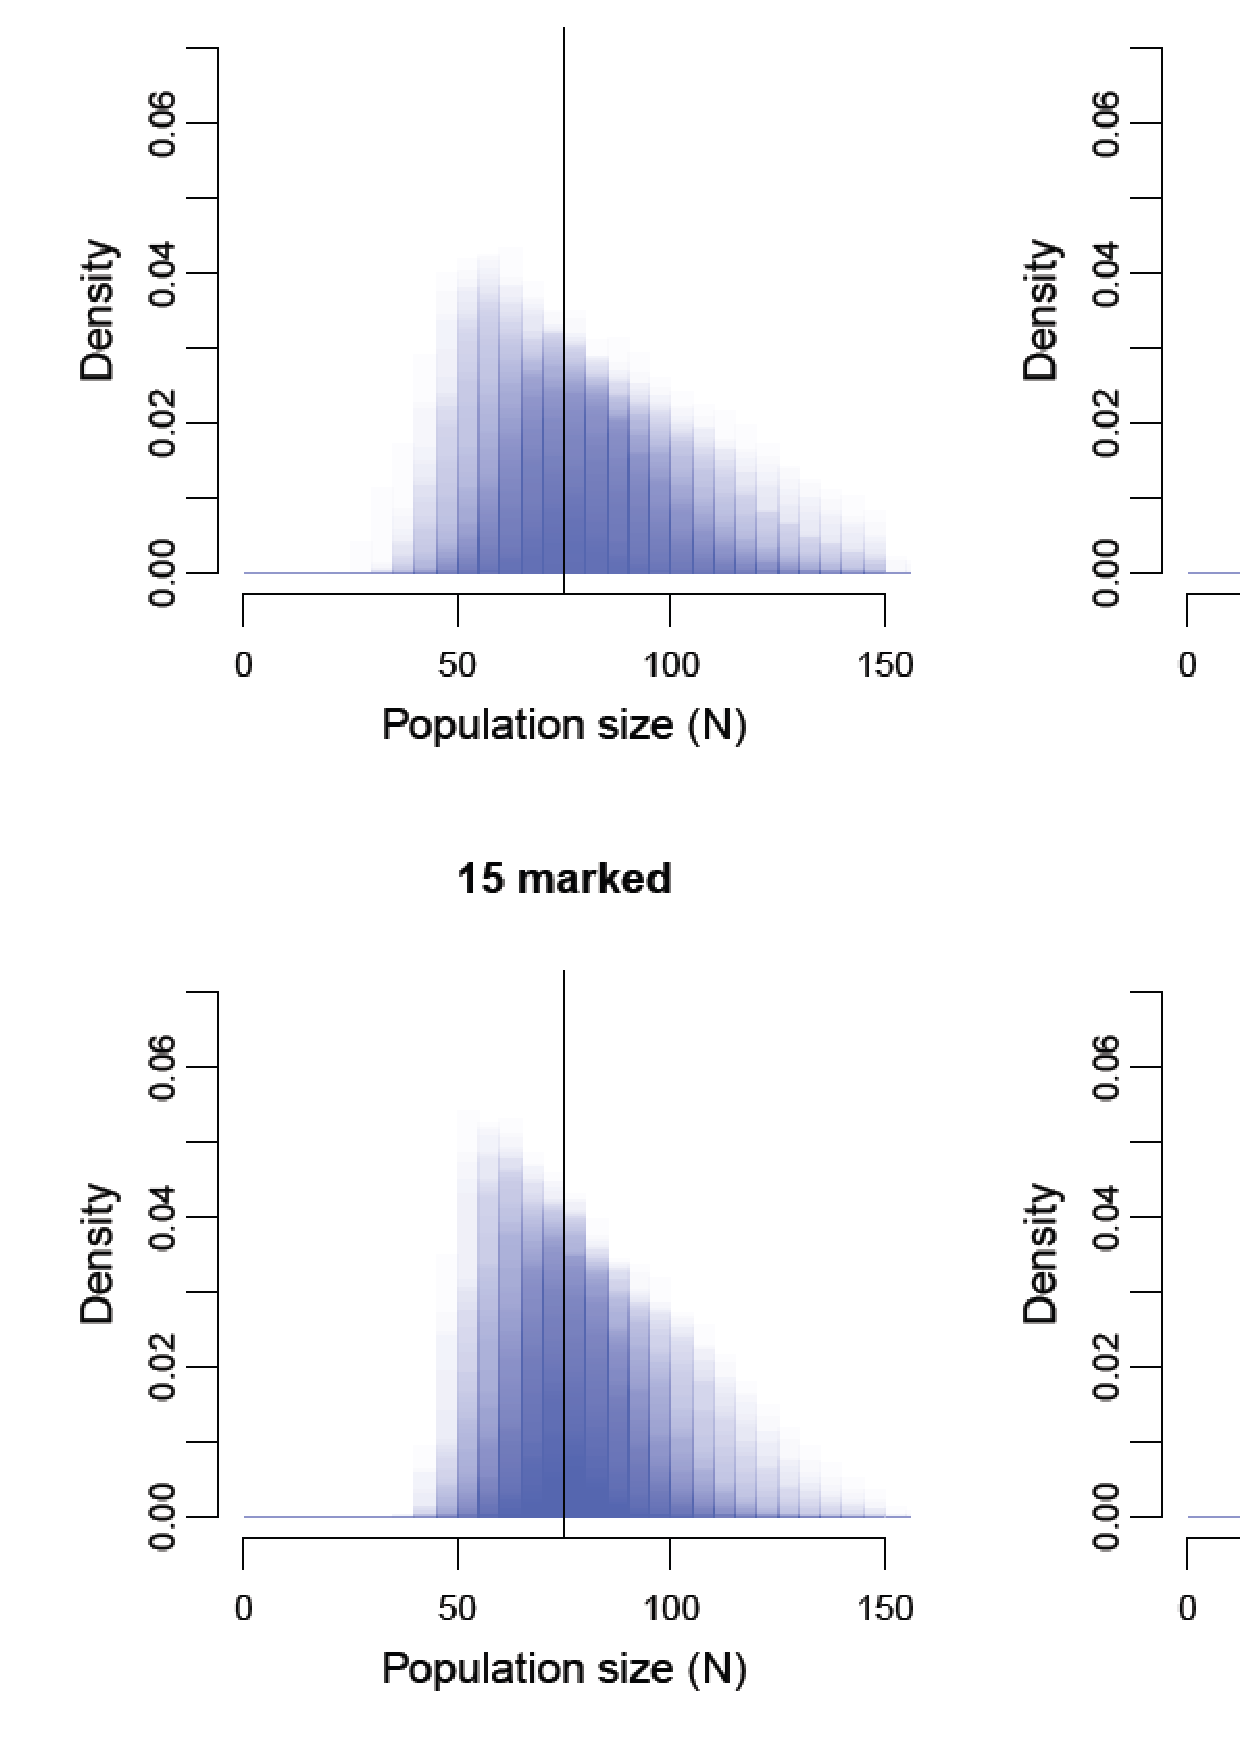
\includegraphics[width=4in,height=4in]{Ch19-PartialID/figs/Nposts2.png}
  \caption{Overlaid posterior distributions of $N$ from 100 simulations
    for four levels of marked individuals.}
  \label{partialID.fig.nposts}
\end{figure}

Without any marked individuals in the population, the posterior
distribution of $N$ turned out to be highly skewed, but the mode was
still an approximately (frequentist) unbiased point estimator of
$N$. As anticipated, posterior precision increased substantially with
the proportion of marked individuals (Table \ref{partialID.tab.sim} and
Fig. \ref{partialID.fig.nposts}). The relative root-mean squared
error decreased from 0.246 when no individuals were marked to 0.085
when 35 individuals were marked
(Table \ref{partialID.tab.sim}). Coverage was nominal for all values of
$m$ and posterior skew greatly diminished with increasing $m$ (Table \ref{partialID.tab.sim}).


\begin{table}[ht]
\centering
\caption{Posterior mean, mode, and associated relative RMSE for simulations in
  which $m$ of $N$=75 individuals were marked. One hundred simulations of each case were conducted. Table taken from \citet{chandler_royle:2012} }
\begin{tabular}{llrrrrr}
     \hline
     &	Parameter    &	Mean   &	rRMSE  & Mode   & rRMSE &	BCI    \\
     \hline
 m=0 &	$N$          &	85.866 &    0.259 & 77.720 &    0.242 & 0.950  \\
     &	$\lambda_0$  &	0.506  &	0.180 &	0.488  &	0.182 &	0.960  \\
     &	$\sigma$     &	0.495  &	0.115 &	0.486  &	0.113 &	0.960  \\
     \hline
 m=5 &	$N$          &	80.898 &    0.184 & 76.360 &    0.182 & 0.970  \\
     &	$\lambda_0$  &	0.510  &    0.178 & 0.494  &    0.180 & 0.950  \\
     &	$\sigma$     &	0.496  &    0.089 & 0.488  &    0.086 & 0.970  \\
     \hline
 m=15&	$N$          &	79.028 &    0.148 & 76.250 &    0.147 & 0.950  \\
     &	$\lambda_0$  &	0.508  &    0.163 & 0.494  &    0.164 & 0.950  \\
     &	$\sigma$     &	0.496  &    0.073 & 0.492  &    0.071 & 0.970  \\
     \hline
 m=25&	$N$          &	77.765 &    0.114 & 75.810 &    0.113 & 0.950  \\
     &	$\lambda_0$  &	0.511  &    0.153 & 0.498  &    0.157 & 0.950  \\
     &	$\sigma$     &	0.496  &    0.067 & 0.493  &    0.065 & 0.940  \\
     \hline
 m=35&	$N$          &	76.446 &    0.085 & 74.900 &    0.085 & 1.000  \\
     &	$\lambda_0$  &	0.513  &    0.142 & 0.501  &    0.144 & 0.950  \\
     &	$\sigma$     &	0.497  &    0.056 & 0.493  &    0.057 & 0.940  \\
 \hline
\end{tabular}
\label{partialID.tab.sim}
\end{table}

As we saw in the previous chapter, the spatial correlation in unmarked
counts can be sufficient to obtain estimates of movement and detection
parameters. However, only marked and thus identifiable individuals
provide us with direct information about these parameters and may well
dominate estimates.  To single out the contribution of marked and
unmarked individuals to parameter estimates, we re-ran the same
simulations but let $\sigma$ and $\lambda_0$ be updated based solely
on the data of marked individuals. Results are summarized in
Table \ref{partialID.tab.sim2}.  We see that if we update $\lambda_0$
and $\sigma$ based on marked individuals only, estimates of these
parameters are more biased and less precise. For estimates of $N$,
especially for $m$= 5 and $m$ = 15, we observe a stronger positive
bias, lower accuracy and considerably lower BCI coverage as compared
to when both marked and unmarked individuals contribute to parameter
estimates (Table \ref{partialID.tab.sim2}). Thus, unmarked individuals
do actually contribute noticeably to estimating model parameters. This stands in contrast to non-spatial mark-resight models, where information about the detection parameter comes solely from the encounter histories of the marked individuals.

\begin{table}[ht]
\centering
\caption{Posterior mean, mode, and associated relative RMSE for simulations in
  which $m$ of $N$=75 individuals were marked and unmarked individuals
  did not contribute to estimating $\lambda_0$ and $\sigma$.
  One hundred simulations of each case were conducted. }
\begin{tabular}{llrrrrr}
\hline
     &	Parameter    &	Mean   &	RMSE  &	Mode   &	RMSE &	BCI    \\
     \hline
 m=5 &	$N$          &	88.621 &	0.369 &	83.139 &	0.421 &	0.810  \\
     &	$\lambda_0$  &	1.255  &	1.247 &	0.606  &	1.148 &	0.950  \\
     &	$\sigma$     &	0.472  &	0.252 &	0.426  &	0.333 &	0.910  \\
     \hline
 m=15&	$N$          &	81.031 &	0.192 &	78.361 &	0.175 &	0.820  \\
     &	$\lambda_0$  &	0.535  &	0.281 &	0.476  &	0.284 &	0.970  \\
     &	$\sigma$     &	0.503  &	0.109 &	0.490  &	0.107 &	0.940  \\
     \hline
 m=25&	$N$          &	78.206 &	0.129 &	76.594 &	0.123 &	0.920  \\
     &	$\lambda_0$  &	0.531  &	0.204 &	0.496  &	0.202 &	0.960  \\
     &	$\sigma$     &	0.497  &	0.081 &	0.489  &	0.084 &	0.950  \\
     \hline
 m=35&	$N$          &	76.833 &	0.099 &	75.422 &	0.096 &	0.940  \\
     &	$\lambda_0$  &	0.528  &	0.192 &	0.505  &	0.186 &	0.940  \\
     &	$\sigma$     &	0.499  &	0.069 &	0.493  &	0.070 &	0.960  \\
 \hline
\end{tabular}
\label{partialID.tab.sim2}
\end{table}


\section{Incorporating telemetry data}
\label{partialID.sec.telemetry}

As we expected, parameter estimates of spatial mark-resight models get
better the more marked individuals we have in our study
population. While this is great advice in theory, it may not be very
helpful in practice, especially when dealing with animals that are
hard or somewhat dangerous to capture, such as large
carnivores. Oftentimes, studies involving the physical capture of such
animals will employ telemetry tags in order to learn about the study
species' spatial ecology and behavior. In the context of spatial
mark-resight models, the actual locations
collected by telemetry tags can provide detailed information on individual location and movement, and being able to incorporate this information directly into the SMR model should improve estimates of these parameters, especially when resighting information is sparse.

%% XXXXX Andy: seems like a cite to the JAPPLE paper would be good
%% around here?
% XX RS: We cite it in the last paragraph of this section.

So how could we combine resighting data and telemetry data in a
unified mark-resight model? Recall that the basic SCR model underlying
all the SMR models we discuss here uses a Gaussian kernel to describe
the trap encounter model.  By using this function, we can relate the
parameters $\sigma$ and ${\bf s}_{i}$ directly to those from a
bivariate normal model of space usage, with mean = ${\bf s}_{i}$, and
variance-covariance matrix ${\bm \Sigma}$, where the variance in both
dimensions is $\sigma^2$ and the covariance is 0. Ordinarily, these
parameters are estimated directly from the spatial distribution of
individual captures/resightings. Telemetry data, however, provide more
detailed information on individual location and movement, since the
resolution and extent of the data are not limited by the trapping grid
and potentially more locations can be accumulated through telemetry
than resighting (depending on the monitoring frequency and resighting
rates of individuals).

By assuming that the $R_i$ locations of individual $i$, ${\bf l}_{i}$ (consisting of a pair of x and y coordinates, $l_{ix}$ and $l_{iy}$), are a bivariate normal (BVN) random variable:
\[
{\bf l}_i\sim {\mbox BVN} ({\bf s}_i,{\bm \Sigma})
\]
we can estimate $\sigma$ as well as ${\bf s}_{i}$ for the collared individuals directly from telemetry locations, using their full conditional distributions:
\[
[\sigma|{\bf l},{\bf s}] \propto \left\{\prod_{i=1}^m \prod_{r=1}^{R_{i}} \frac{1}{2 \pi \sigma^2} {\exp}\left(-1/2 \left[ \frac {(l_{irx}-s_{ix})^2} {\sigma^2} + \frac{(l_{iry}-s_{iy})^2}{\sigma^2} \right]\right)\right\}*[\sigma]
\]
and
\[
[{\bf s}_i|{\bf l},\sigma] \propto \left\{\prod_{r=1}^{R_{i}} \frac{1}{2 \pi \sigma^2} {\exp}\left(-1/2 \left[ \frac {(l_{irx}-s_{ix})^2} {\sigma^2} + \frac{(l_{iry}-s_{iy})^2}{\sigma^2} \right]\right)\right\}*[{\bf s}_{i}]
\]

For the unmarked individuals ${\bf s}_{i}$ are estimated as described
before conditional on their latent encounter histories.  Note that the
bivariate normal model assumes that locations are independent of each
other. If you have frequent telemetry fixes, for example from GPS
collars that report animal locations every few hours or more, this
assumption seems unrealistic and it might be advisable to thin your
telemetry data (maybe to daily fixes) in order to approximate
independence.  Alternatively, movement models could be used that
acknowledge the temporal correlation in location data. We suggested
some possible movement models in Chapt. \ref{chapt.search-encounter}.
Not all marked individuals need to be telemetry-tagged, but telemetry
data should correspond to the period over which resighting surveys
were conducted (as we discussed in Chapt. \ref{chapt.scr0}, both the
${\bf s}_i$ and $\sigma$ should only be interpreted against the
specific sampling period). Further, telemetry data need to be
independent of the resighting data.

Again, implementation of this model extension is straight-forward,
both in {\bf JAGS} and {\bf R}. Take the SMR model description for the
case where $m$ is known (Panel \ref{partialID.panel.knownm}). Then,
all we have to do is add a description of the bivariate normal model
for the telemetry locations, here {\tt locs}, into the loop over the
$m$ marked individuals:
{\small
\begin{verbatim}
[...parts of model code omitted...]

for(i in 1:m) {

  sm[i,1] ~ dunif(xlim[1], xlim[2])
  sm[i,2] ~ dunif(ylim[1], ylim[2])

  #telemetry model
  for (r in off1[i]:off2[i]){
  locs[r,1]~dnorm(sm[i,1], 1/(sigma^2))
  locs[r,2]~dnorm(sm[i,2], 1/(sigma^2))
  }

  for(j in 1:J) {
    distm[i,j] <- sqrt((sm[i,1]-X[j,1])^2 + (sm[i,2]-X[j,2])^2)
    lambdam[i,j] <- lam0*exp(-distm[i,j]^2/(2*sigma^2))
    y[i,j]~dpois(lambdam[i,j]*K)
    }
  }

[...parts of model code omitted...]
\end{verbatim}
}
The data object {\tt locs} is a table with all $\sum_i^m R_i$
telemetry locations. The two vectors {\tt off1} and {\tt off2}
describe which subset of this matrix belongs to individual $i$. So if,
say, the locations for individual 1 are contained in the first 10 rows
of {\tt locs}, {\tt off1} and {\tt off2} would be 1 and 10 for $i=1$;
and if the locations of individual 2 are in the following 15 rows,{\tt
  off1} and {\tt off2} for $i=2$ would be 11 and 25, and so on. For
the implementation of this SMR model with telemetry data in {\bf R},
see the {\tt scrPID.tel} function in {\tt scrbook}. In a nutshell, in
the MCMC algorithm we replaced the Metropolis-Hastings updating steps
for $\sigma$ and activity centers, ${\bf s}_i$, of marked individuals, which were originally
conditional on the resighting data, with updating steps conditional on
the telemetry data. This is not quite what the above {\bf JAGS} code
does; rather {\bf JAGS} will update these parameters conditional on
both the telemetry \emph{and} the resighting data. We could easily
re-write {\tt scrPID.tel} to do that, but believe that for most
applications, the information on location and movement contained in
the telemetry data will outweigh that in the resighting data, so that
the resulting loss of information should be minimal.

\subsection{Raccoons on the Outer Banks of North Carolina}

\citet{sollmann_etal:2012ecol} applied a spatial mark-resight model
with telemetry data to a camera-trap and radio-telemetry data set from
the raccoon population on South Core Banks, a barrier island within
Cape Lookout National Seashore, North Carolina. Between May and
September 2007, 131 raccoons were marked with dog collars and large
individually numbered cattle tags. Individuals were marked throughout
the island, so that (a) we do not have to deal with sensitivity to
choice of the state-space, because it is clearly defined by nature;
and (b) it is reasonable to assume that marked raccoons are a random
sample of individuals from this state-space.  Of the 131 tagged
individuals, 44 were also equipped with radio collars. Collared
individuals were located using a VHF receiver and antenna, and their
locations were estimated approximately weekly. Twenty camera traps
were set up along the length of South Core Banks and camera trapping
data collected between October 1 2007 to January 22 2008 constituted
the resighting data in this analysis. During this period 104 marked
individuals, 38 radio-collared, were alive and available for
resighting with camera traps.

\begin{figure}[ht]
  \centering
  \includegraphics[width=4in]{Ch19-PartialID/figs/Raccoon_pic.png}
  \caption{Camera trap picture of a raccoon marked with a cattle tag that cannot be read to determine individual identity. Taken on South Core Banks, North Carolina.
({\it Photo credit: Arielle Parsons})}
  \label{partialID.fig.raccoon}
\end{figure}

The state-space ${\cal S}$ was the entire area of South Core Banks
island. A change in the number of photocaptures over the course of the
study suggested a variation of detection rate with time. Since date
recording in cameras malfunctioned, photographic records could only be
assigned to the time interval between subsequent trap checks, and
these intervals between checks are referred to as sampling
occasions. These occasions ranged from 2 to 43 days; $\lambda_0$ was
standardized to 7-day intervals and allowed to change with sampling
occasion. Since not all pictures of marked raccoons could be
identified to the individual level, the authors applied the correction
factor $c$ as described in Sec. \ref{partialID.sec.IDrate}, estimated
separately for each occasion.

Camera-traps recorded 117 pictures of unmarked raccoons, 33 pictures
of 18 marked and identifiable raccoons, and 49 records of marked but
not individually identifiable individuals
(Fig. \ref{partialID.fig.raccoon}). An average of 16.32 telemetry
locations (SD 4.91) were collected for each of the 38 collared
individuals. Raccoon abundance on the island was estimated at 186.71
(SE 14.81) individuals, which translated to a density of 8.29 (SE
0.66) individuals per km$^2$. Parameter estimates are listed in
Table \ref{partialID.tab.raccoons}.

\begin{table}%[hb]
\centering
\caption{Summary statistics of posterior distributions
  from spatial mark-resigh model for raccoon camera trapping and telemetry data. Baseline trap encounter rate $\lambda_0$ was standardized to 7-day intervals; $\lambda_0$ and the probability of identifying a picture of a marked individual, $c$, were allowed to vary among the 6 sampling occasions (t); $\sigma$ is estimated from telemetry data of 38 radio-collared individuals.}
\begin{tabular}{lrrrrr}
\hline
   &	Mean (SE) &	2.5\% &	50\%	& 97.5\% \\
 \hline
$N$	& 186.71 (14.81) & 162 & 185	& 220 \\
$D$	& 8.29 (0.66)	& 7.19	& 8.22	& 9.77 \\
$\lambda_0$ (t=1)	& 0.24 (0.05) & 0.16 & 0.23 & 0.34 \\
$\lambda_0$ (t=2)	& 0.40 (0.08)	& 0.26	& 0.39	& 0.57 \\
$\lambda_0$ (t=3)	& 0.11 (0.03) & 0.06 & 0.11	& 0.17 \\
$\lambda_0$ (t=4)	& 0.30 (0.07)	& 0.17	& 0.29	& 0.46 \\
$\lambda_0$ (t=5)	& 0.03 (0.01)	& 0.02	& 0.03	& 0.06 \\
$\lambda_0$ (t=6)	& 0.03 (0.01)	& 0.02	& 0.03	& 0.05 \\
$\sigma$	& 0.49 (0.01)	& 0.47	& 0.49	& 0.51 \\
$c$ (t=1)	& 0.55 (0.09)	& 0.38	& 0.55	& 0.71 \\
$c$ (t=2)	& 0.39 (0.11)	& 0.18	& 0.39	& 0.62 \\
$c$ (t=3)	& 0.29 (0.11) & 0.11	& 0.29	& 0.52 \\
$c$ (t=4)	& 0.38 (0.16)	& 0.10	& 0.36	& 0.71 \\
$c$ (t=5)	& 0.38 (0.16)	& 0.10	& 0.36	& 0.71 \\
$c$ (t=6)	& 0.30 (0.14)	& 0.08	& 0.29	& 0.60 \\
 \hline
\end{tabular}
\label{partialID.tab.raccoons}
\end{table}

In this study, although a large number of raccoons were tagged,
photographic data of these tagged individuals were surprisingly
sparse. Analysis of the photographic data set without the telemetry
data did not render usable estimates as parallel Markov chains did not
converge. One reason for the relatively sparse data was the camera
trap study design: traps were spaced on average 1.77 km apart, which
is about 3.5 times $\sigma$. Consequently, very few individual
raccoons were photographed at more than one trap. Under these
circumstances, the telemetry data provide the necessary spatial
information to estimate $\sigma$ and the activity centers of
individual animals and thus make other model parameter
estimable. Similarly, in a camera-trapping study on Florida panthers
(\emph{Puma concolor coryi}), \citet{sollmann_etal:inprepjapplecol},
including telemetry data from the 3 individuals that were collared and
known to use the study area resulted in density estimates with
considerably higher precision as compared to preliminary estimates
\emph{without} telemetry location data, reducing the width of the 95
\% BCI by about 60 \%. Such improvements in precision of estimates is
especially important when we are interested in changes in the
population over time.


\section{Point-process models for marked individuals}

As discussed in Sec. \ref{partialID.sec.random}, all previously
developed SMR models assume that marked individuals are a random
sample, both spatially and demographically, from the population of the
state-space. For many studies it may not be feasible to strive to meet
or approximate the assumption of spatial randomness and it is thus
important to generalize SMR models to situations where marking does
not take place throughout ${\cal S}$. We already stated that in this
situation, we generally cannot assume that activity centers of marked
individuals (and unmarked, for that matter) follow a homogeneous
point-process. In this final section, we will describe two possible
approaches to formulating such an inhomogeneous point-process model. We will
only provide conceptual descriptions, not a full-blown model
development, as at the time of writing this book, these approaches are
still somewhat experimental.


\subsection{Homogeneous point-process in a subset of ${\cal S}$}

% XX RS: So I ended up not using the lizard example, because the difference is that in the search encounter you condition on u, but here we say s has to be within the polygon. I think giving the lizard example and the discussing why it's actually not truly an example of this approach would just be confusing.
Imagine we perform an area search in a square, ${\cal B}$, for some species we want to study, maybe a reptile, and we mark all individuals we encounter. We conduct our sampling in a way that we can assume that marked individuals are randomly
sampled within $\mathcal{B}$, and that there are no marked individuals with activity centers outside of ${\cal B}$.
This design entails the assumption that ${\cal B}$ can be clearly defined. We will come back to these assumptions in a minute. We then perform resighting surveys of some sort in an area that overlaps ${\cal B}$, so that, when we set a state-space around the resighting locations, ${\cal B}$ is completely contained within ${\cal S}$ (Fig. \ref{partialID.fig.Box}). We further assume that individuals that were marked in ${\cal B}$ continue to live within ${\cal B}$ when resighting surveys are conducted, i.e. their activity centers do not shift during the complete mark-resight study. This implies population closure across both the marking and the resighting part of the study, and in this situation we can treat the number of marked animals,  $m$, as known.
Let the total population of ${\cal B}$ be $N_B$. Under the conditions specified above, the number of marked animals $m$ can be described as the outcome of a binomial random variable
\[
m \sim \mbox{Binomial}(\theta, N_B)
\]
where $\theta$ is the probability that an animal living in ${\cal B}$ is marked.
Under these conditions we can describe the point-process for marked individuals as uniform across ${\cal B}$, with zero probability of a marked activity center being located outside of ${\cal B}$. If the combined (or marginal) point-process of marked and unmarked individuals is homogeneous across ${\cal S}$ , i.e. overall density is constant, then, colloquially speaking, the point-process for unmarked individuals is the complement of the marked process: outside of ${\cal B}$, unmarked animals occur at the average density of ${\cal S}$, $D$, while inside ${\cal B}$ they occur at $D * (1-\theta)$.

The above
model is an approach to specifying a spatial reference frame for
marked individuals that is independent of ${\cal S}$.
Some of the assumptions of the model, however, are reminiscent of traditional capture-recapture and thus, suffer from the same shortcomings. ${\cal B}$ needs to be clearly defined as the area the marked individuals live in, but how do we define it? Imagine again that ${\cal B}$ is a square search plot. Surely, we could capture an individual at the edge of the plot, whose activity center is located \emph{off} that plot. Not accounting for this effect would overestimate density in ${\cal B}$. This is the equivalent of having to define an effective area sampled in traditional capture-recapture in order to estimate density. Further, we assume that $\theta$, the probability of an individual within the plot being marked, is the same for all individuals in ${\cal B}$. But we discussed early on in this book that this is unlikely to be true, because exposure to sampling depends on an individual's home range overlap with the sampled area. So individuals near the edge of ${\cal B}$ are less likely to be marked than those in the center, assuming we dispense marking effort uniformly across ${\cal B}$. In spite of the shortcomings of this approach, we believe it could serve as a reasonable approximation of some study systems. Moreover, it serves as a conceptual device because it presents a relatively simple way of thinking about two overlapping point processes, in the context of SMR the point-processes describing the distribution of marked and unmarked individuals in ${\cal S}$.


\begin{figure}[ht]
\begin{center}
\includegraphics[width=5in]{Ch19-PartialID/figs/scrPIDBox.png}
\end{center}
\caption{
Relationship between marking area ${\cal B}$ and state-space, ${\cal S}$.
}
\label{partialID.fig.Box}
\end{figure}

\subsection{Bivariate normal distribution around the centroid of the
  marking array}
% XX RC: Rather than call this a "BVN", it would probably be better to
% just call it an inhomogenous point process in which the intensity
% decreases with distance from the traps (or the trap centroid). I
% know, I'm the one that originally called it a BVN, but I don't think
% the BVN is quite right, since we want an intensity function that
% when integrated over space, returns the expected value of N (or m).
An alternative, and more realistic, inhomogeneous point-process for marked individuals is one that describes a decline in the density of marks with increasing distance to the marking location(s). We would expect this kind of spatial pattern in marks to arise, because animals living in the center of the marking grid have a higher probability to be marked than those living on the edges, which in turn have a higher marking probability than those living beyond the marking grid. As a consequence, the density of marks is higher near the centroid of the marking grid and decreases as we move a away from it. Imagine that marking of animals takes place across some area or grid, and let $C_m$ be the centroid of that marking area. Then, a plausible model for the distribution of marked animals  is a bivariate normal model with mean $C_m$ and variance-covariance matrix, ${\bm \Sigma_C}$, where the variance in both
dimensions is $\sigma_C^2$ and the covariance is 0 (Fig. \ref{partialID.fig.hn}).
Of course, there are alternative models to describe a decrease in density, such as a negative-exponential or hazard function. Once the distribution of marked animals conditional on $C_m$ is adequately described, the
inhomogeneous point-process for the unmarked animals can again be modeled by assuming that the marginal density across ${\cal S}$ is constant, similar to the example above.
% XXX RC: You could also say that the parameters of the IPP could be
% modeled using the methods in Ch11.
% XXX RC: Also, it might be worth noting that density should be
% invariate to the size of S, as long as it is big enough.

While this model formulation is more realistic and general, it has some minor drawbacks. Based on very limited experience, the variance parameter, $\sigma_C^2$, is barely estimable under realistic sample sizes. This is not surprising, given that this parameter attempts to describe the distribution of the activity centers, which are themselves latent. Further, the approach does entail some design constraints for marking. We implicitly assume that the centroid of the marking array is the area of highest probability of being marked, which means that marking effort has to be somewhat constant across the marking area. The assumption seems reasonable for systematic or random marking arrays (Fig. \ref{partialID.fig.hn}), but, for example, for a ``hollow grid'' the centroid would not be an adequate representation of the point of highest marking probability.
The take-home message here is that the adequate point-process model for the distribution of marks depends on the spatial context of the marking process.

{\flushleft \bf Moving activity centers:} One issue we have not addressed explicitly in this section is what to do when enough time passes between marking and resighting so that animals may have rearranged themselves spatially. In example 1 this could mean, marked animals have shifted their activity center outside of the marking plot ${\cal B}$. In the second example, marked animals may no longer follow that initial distribution around the centroid of the marking array. Irrespectively, we will have to make some assumption about how marked individuals are distributed in space. We saw such a case in the Canada geese example in Sec. \ref{partialID.subsec.geese}. In that example, we defined a reasonable state-space and assumed that animals redistributed themselves randomly across that state-space between marking and resighting, because they were capture while moulting. This seems like a sensible solution for that particular study system, but it leads to a model formulation where estimates of density are sensitive to choice of ${\cal S}$. Alternatively, we could again use a bivariate normal distribution around the centroid of the original marking array -- if movement of activity centers is random with respect to $C_m$ it seems plausible that the overall underlying distribution of $\bf s$ would still be adequately described with a bivariate normal model.
% XX RS: Feel free to delete, I am improvizing here
You see that now, choice of a model for the inhomogeneous point-process of marked individuals depends both on the spatial context of marking and what we know (or believe) about the biology of the study species.

% XXX RC: Consider changing the axis labels since we use "X" and "Y" for other things
\begin{figure}[htp]
\begin{center}
\includegraphics[width=5in]{Ch19-PartialID/figs/scrPIDhn.png}
\end{center}
\caption{
Plot of activity centers of marked (black dots) and unmarked (gray dots) individuals, with marked individuals following a bivariate normal distribution around the centroid (asterisk) of the marking locations (+); the marginal point-process of both marked and unmarked individuals combined is homogeneous.
}
\label{partialID.fig.hn}
\end{figure}




\section{Summary and Outlook}

In this chapter we combined SCR models (for marked individuals) with a
model for unmarked individuals,
to derive a spatial mark-resight (SMR) model, which
accommodates that only part of the population is individually identifiable,
usually through artificial tags. Under the assumption that marked
individuals are a random sample, both demographically and spatially,
from the state-space, the basic model with known number of marked
individuals and perfect individual identification of marks
is easily
modified for situations where the number of marked individuals is
unknown, or where marked animals can sometimes not be identified to
individual level. As expected, having marked individuals in the study
population improved accuracy and precision of parameter estimates when
compared to fully unmarked populations, but we also saw that the
spatial counts of unmarked individuals still contribute information to
parameter estimates. Finally, we presented an approach to
incorporate telemetry location data into the spatial mark-resight
model to inform estimates of $\sigma$ and activity centers. Just as in
SCR, the spatial mark-resight models can account for a variety of
factors that may influence individual movement and detection, as well
as survey-related parameters, and we saw one example for the Canada
geese, where $\sigma$ was sex-specific.

Many details of SMR models remain to be explored. We mentioned the
assignment of marked but unidentified records to actual marked
individuals based on their spatial location, which provides some
(though imperfect) information of their identity
(Sec. \ref{partialID.sec.IDrate}). Similarly, records where the marked
status cannot be determined could potentially be included in the model
as some form of overall correction factor on detection. GPS telemetry
devices and their ability to collect location data with much higher
frequency offer the opportunity to assign records of collared animals
to individuals based on how close to a given camera the collared
individuals were, both in space and time. In this scenario, individual
identity itself could be expressed probabilistically, leading to an
SMR model accounting for potential misidentification. All these
possible extensions can tailor SMR models to specific survey
techniques.

A fundamental assumption of all the SMR models developed in this
chapter was that marked animals are a random sample from ${\cal
  S}$. This simplifies the model as we can assume a homogeneous point
process for both the marked and the unmarked part of the
population. While this is a convenient situation, it is neither likely
to arise often in real life, nor strictly necessary.  If marked
animals are not a random sample from ${\cal S}$, we need to describe
their distribution in the state-space using an adequate point-process
that will almost always be inhomogeneous across ${\cal S}$.  We
mention two possible approach -- a uniform (homogeneous) point process
over a smaller area within ${\cal S}$, and a bivariate normal
distribution around the centroid of the marking locations, so that
density of marked animals decreases with distance to that centroid.
Both formulations effectively attempt to describe the distribution of
marks in space as a consequence of the spatial nature of the marking
process. We believe that another way to approach this problem is to
combine spatially explicit models for the marking process and the
resighting process. Where marked animals were captured carries
information on their spatial distribution, and it should be possible
to make use of this information by formulating an integrated spatial
capture-mark-resighting model. Such approaches have been developed in
a non-spatial CR framework \citep{matechou_etal:2013,
  pledger_etal:2009}, but to our knowledge have not yet been addressed
in the context of SCR.

 Spatial mark-resight models are a recent
development, and work on how to relax the spatial component of the
random sample assumption and formulate adequate point-process models for the distribution of marks is ongoing. While there is still a lot of work to be done, we believe that SMR modeling holds the
potential to address a wide range of population estimation problems
when dealing with animals that cannot be identified based on natural
marks, a situation that is typical of a majority of animal population
studies.












\bibliography{AndyRefs_alphabetized}

\end{document}